\section{User Manual}

\subsection{Sign in}
\begin{figure}[H]
	\centering
	
\includegraphics[width=1.\linewidth]{graphics/gui/user/landing}
	\caption{Landing Page}
	\label{fig:landing}
\end{figure}

In the landing page of the service, navigate to Login page by clicking "Sign In Now"


\begin{figure}[H]
	\centering
	\begin{minipage}{.5\textwidth}
		\centering
		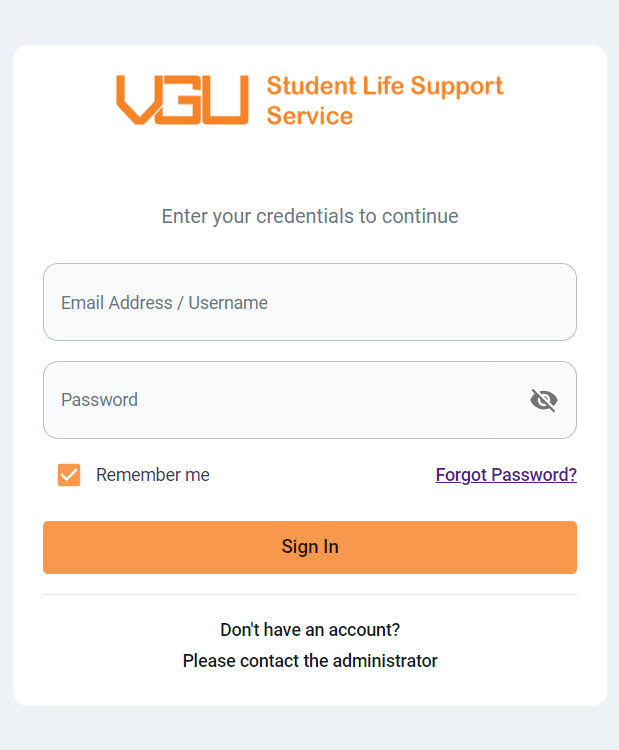
\includegraphics[width=.9\linewidth]{graphics/gui/user/login.png}
		\captionof{figure}{Sign in Form}
		\label{fig:gui-login}
	\end{minipage}%
	\begin{minipage}{.5\textwidth}
		\centering
		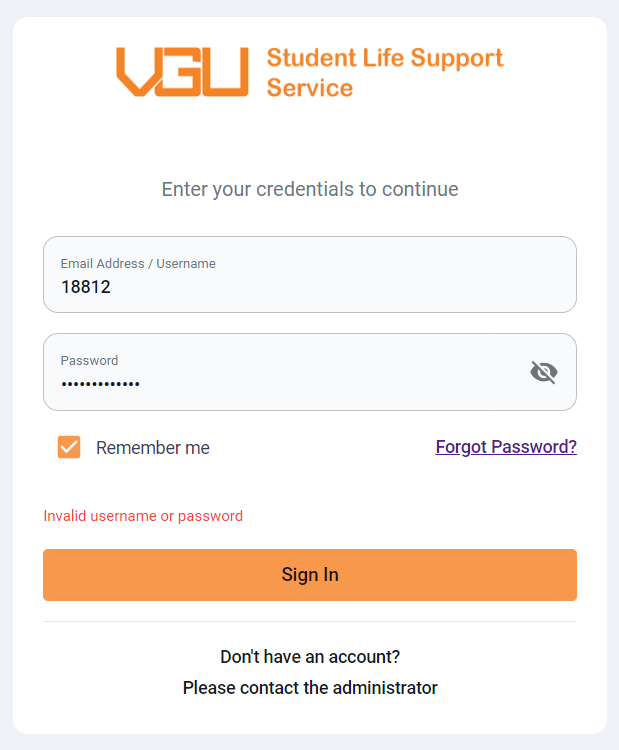
\includegraphics[width=0.9\linewidth]{graphics/gui/user/login-error.png}
		\captionof{figure}{Failed Sign in attempt}
		\label{fig:gui-login-failed}
	\end{minipage}
\end{figure}



To access the service, input your username (or email) and password, then click on the sign-in button (refer to Figure \ref{fig:gui-login}). If you provide incorrect credentials, a warning message will appear, indicating that you need to correct either your username or password (Figure \ref{fig:gui-login-failed}).





\subsection{Forgot password}

%In case of forgetting your password, you can reset it by clicking 'Forgot Password?' of the 'Sign in' form (see Firgure \ref{fig:gui-login}). Then, enter your the email in the 'Forgot Password' form adn click 'Reset Password' (Figure \ref{fig:gui-forgot-pass})

If you forget your password, you can initiate a reset by selecting the 'Forgot Password?' option on the 'Sign in' form (refer to Figure \ref{fig:gui-login}). Subsequently, provide your email address in the 'Forgot Password' form and click on 'Reset Password' (see Figure \ref{fig:gui-forgot-pass}).

\begin{figure}[H]
	\centering
	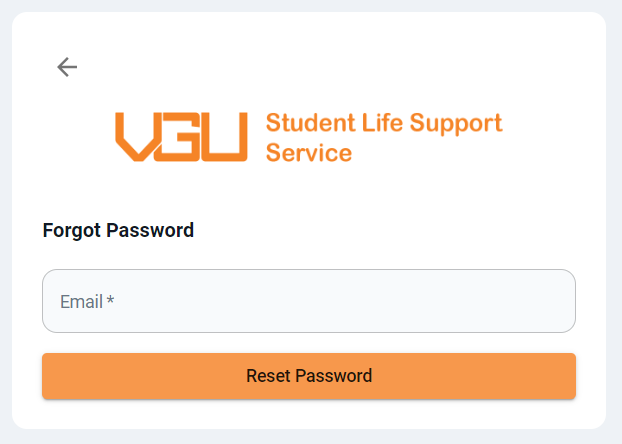
\includegraphics[width=0.7\linewidth]{graphics/gui/user/reset-pass.png}
	\caption{Reset Password Form}
	\label{fig:gui-forgot-pass}
\end{figure}



If your email is associated with an account in the system, a success notification will appear, and password reset instructions will be sent to your email (Figure \ref{fig:gui-reset-pass-success}, \ref{fig:gui-email-reset-pass}).  Conversely, if the email is not found in the system, a failure notification will indicate that the email does not exist (Figure \ref{fig:gui-reset-pass-failed}).

\begin{figure}[H]
	\centering
	\begin{minipage}{.5\textwidth}
		\centering
		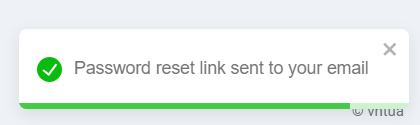
\includegraphics[width=.9\linewidth]{graphics/gui/user/reset-pass-success.png}
		\captionof{figure}{Reset password successfully}
		\label{fig:gui-reset-pass-success}
	\end{minipage}%
	\begin{minipage}{.5\textwidth}
		\centering
		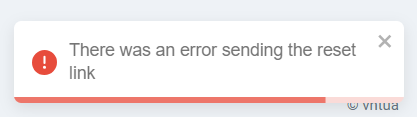
\includegraphics[width=0.9\linewidth]{graphics/gui/user/reset-pass-failed.png}
		\captionof{figure}{Reset password failed}
		\label{fig:gui-reset-pass-failed}
	\end{minipage}
\end{figure}


\begin{figure}[H]
	\centering
	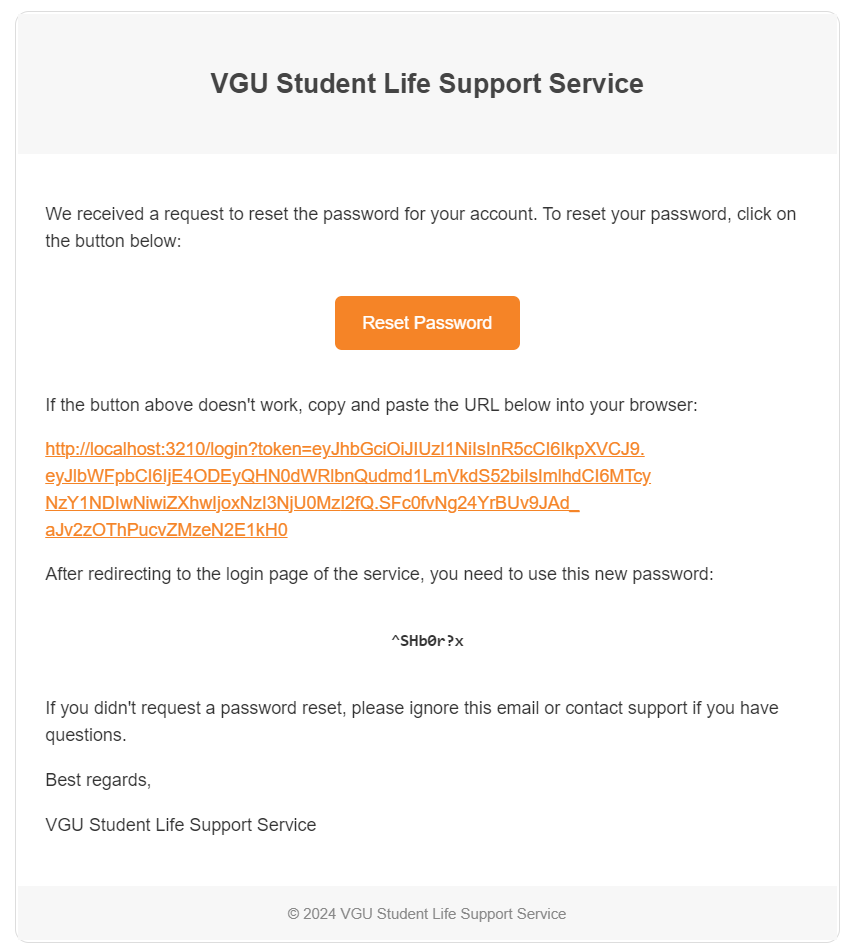
\includegraphics[width=0.8\linewidth]{graphics/gui/user/email-reset.png}
	\caption{Reset password email instructions}
	\label{fig:gui-email-reset-pass}
\end{figure}


\subsection{Student's functions}
After logging in successfully, students will be navigated to the homepage

\begin{figure}[H]
	\centering
	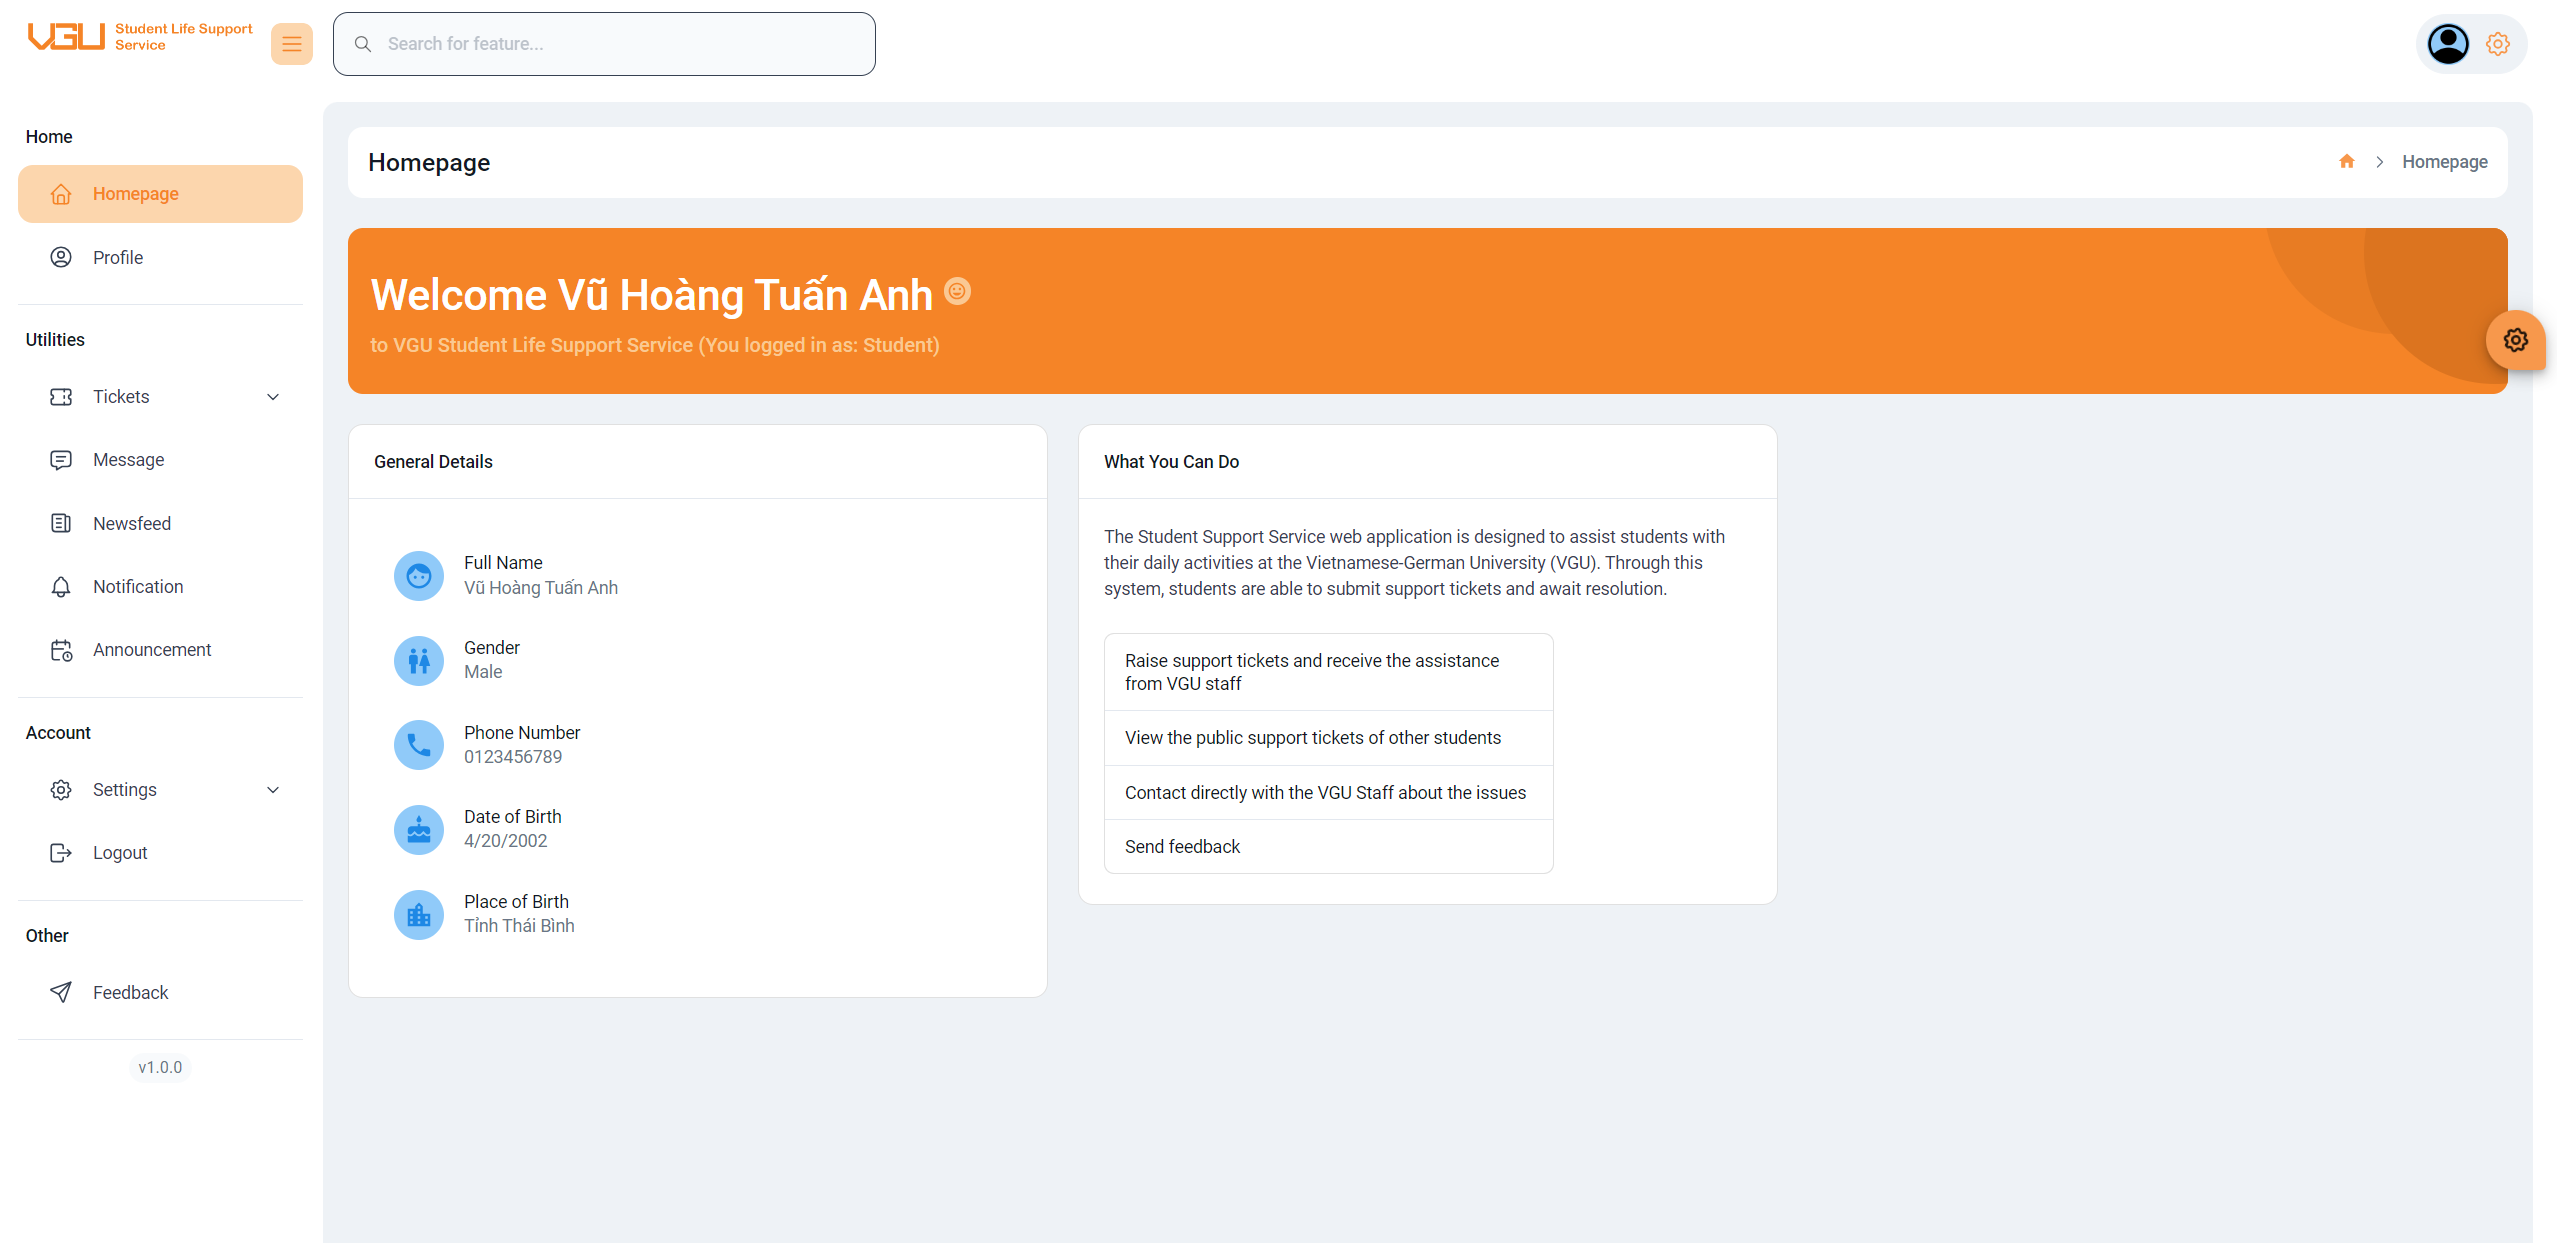
\includegraphics[width=1.0\linewidth]{graphics/gui/student/homepage}
	\caption{Student's Home Page}
	\label{fig:gui-std-homepage}
\end{figure}


	\subsubsection{View Profile}
	\begin{figure}[H]
		\centering
		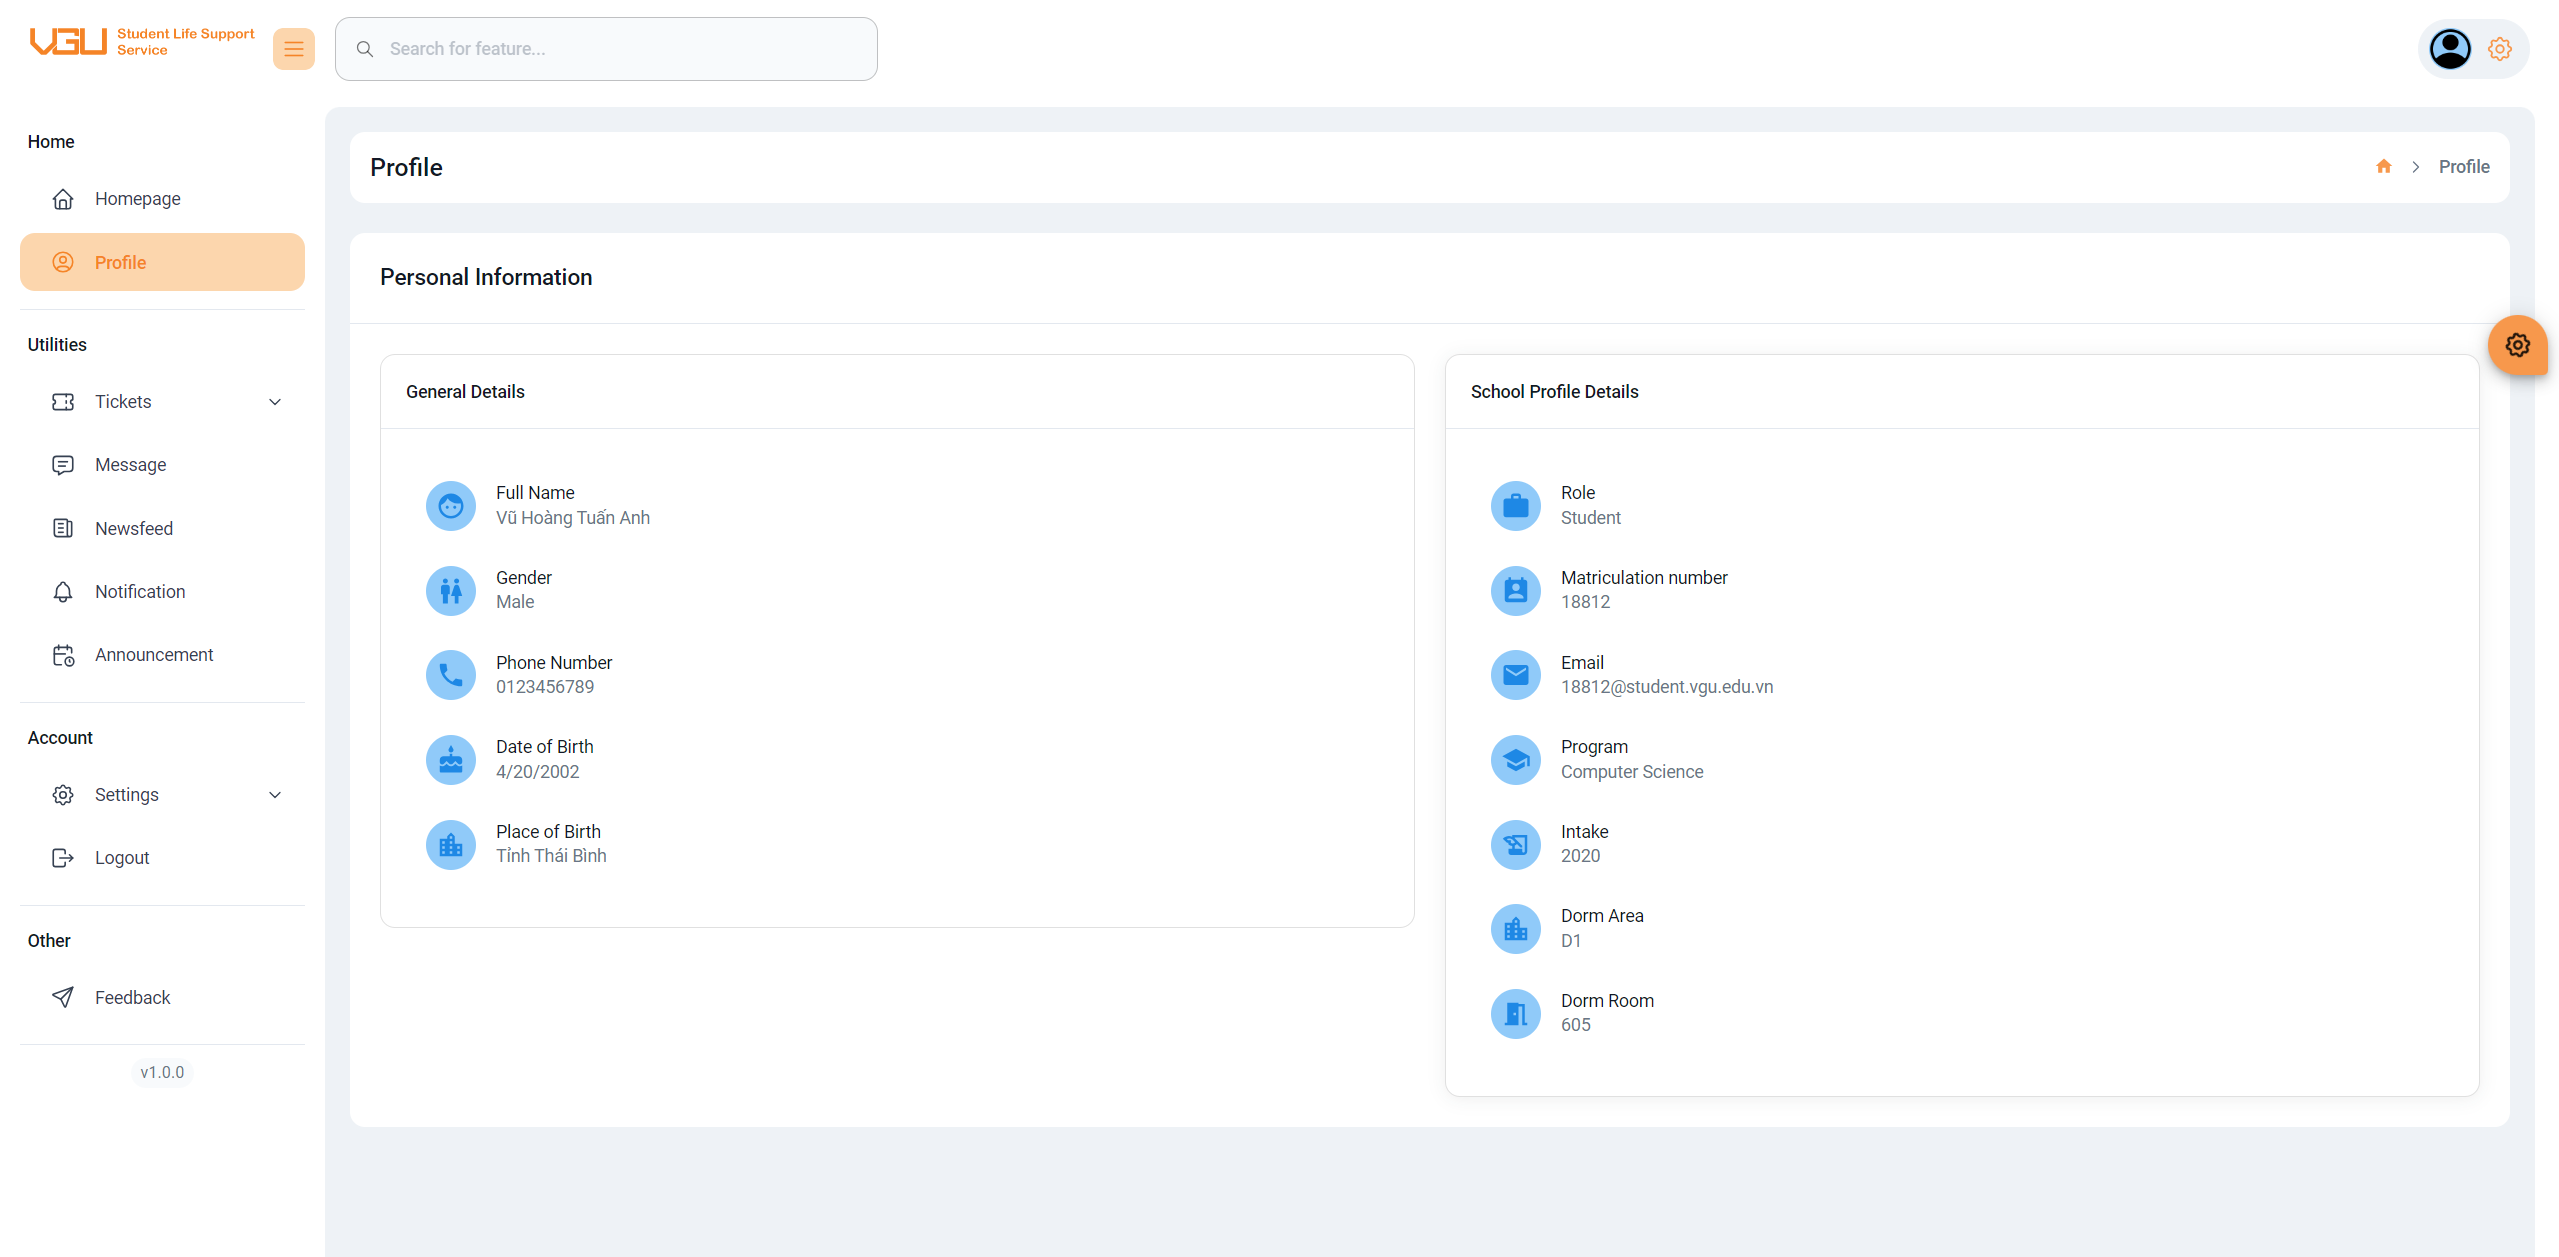
\includegraphics[width=1.0\linewidth]{graphics/gui/student/profile}
		\caption{Student's Profile Page}
		\label{fig:gui-std-profile}
	\end{figure}
	Students can access their personal information through the "Profile" menu. This section provides an overview of their personal details, allowing students to view and manage their account-related information.
	
	
	
	
	\subsubsection{View Tickets}

	Students can access their tickets by navigating to \texttt{Tickets > My Tickets}. This page displays a table listing all of the students' tickets along with a ticket details panel. To view the details of a specific ticket, students can click the visibility icon corresponding to the selected ticket in the table. (see Figure \ref{fig:gui-std-my-tickets})
	\begin{figure}[H]
		\centering
		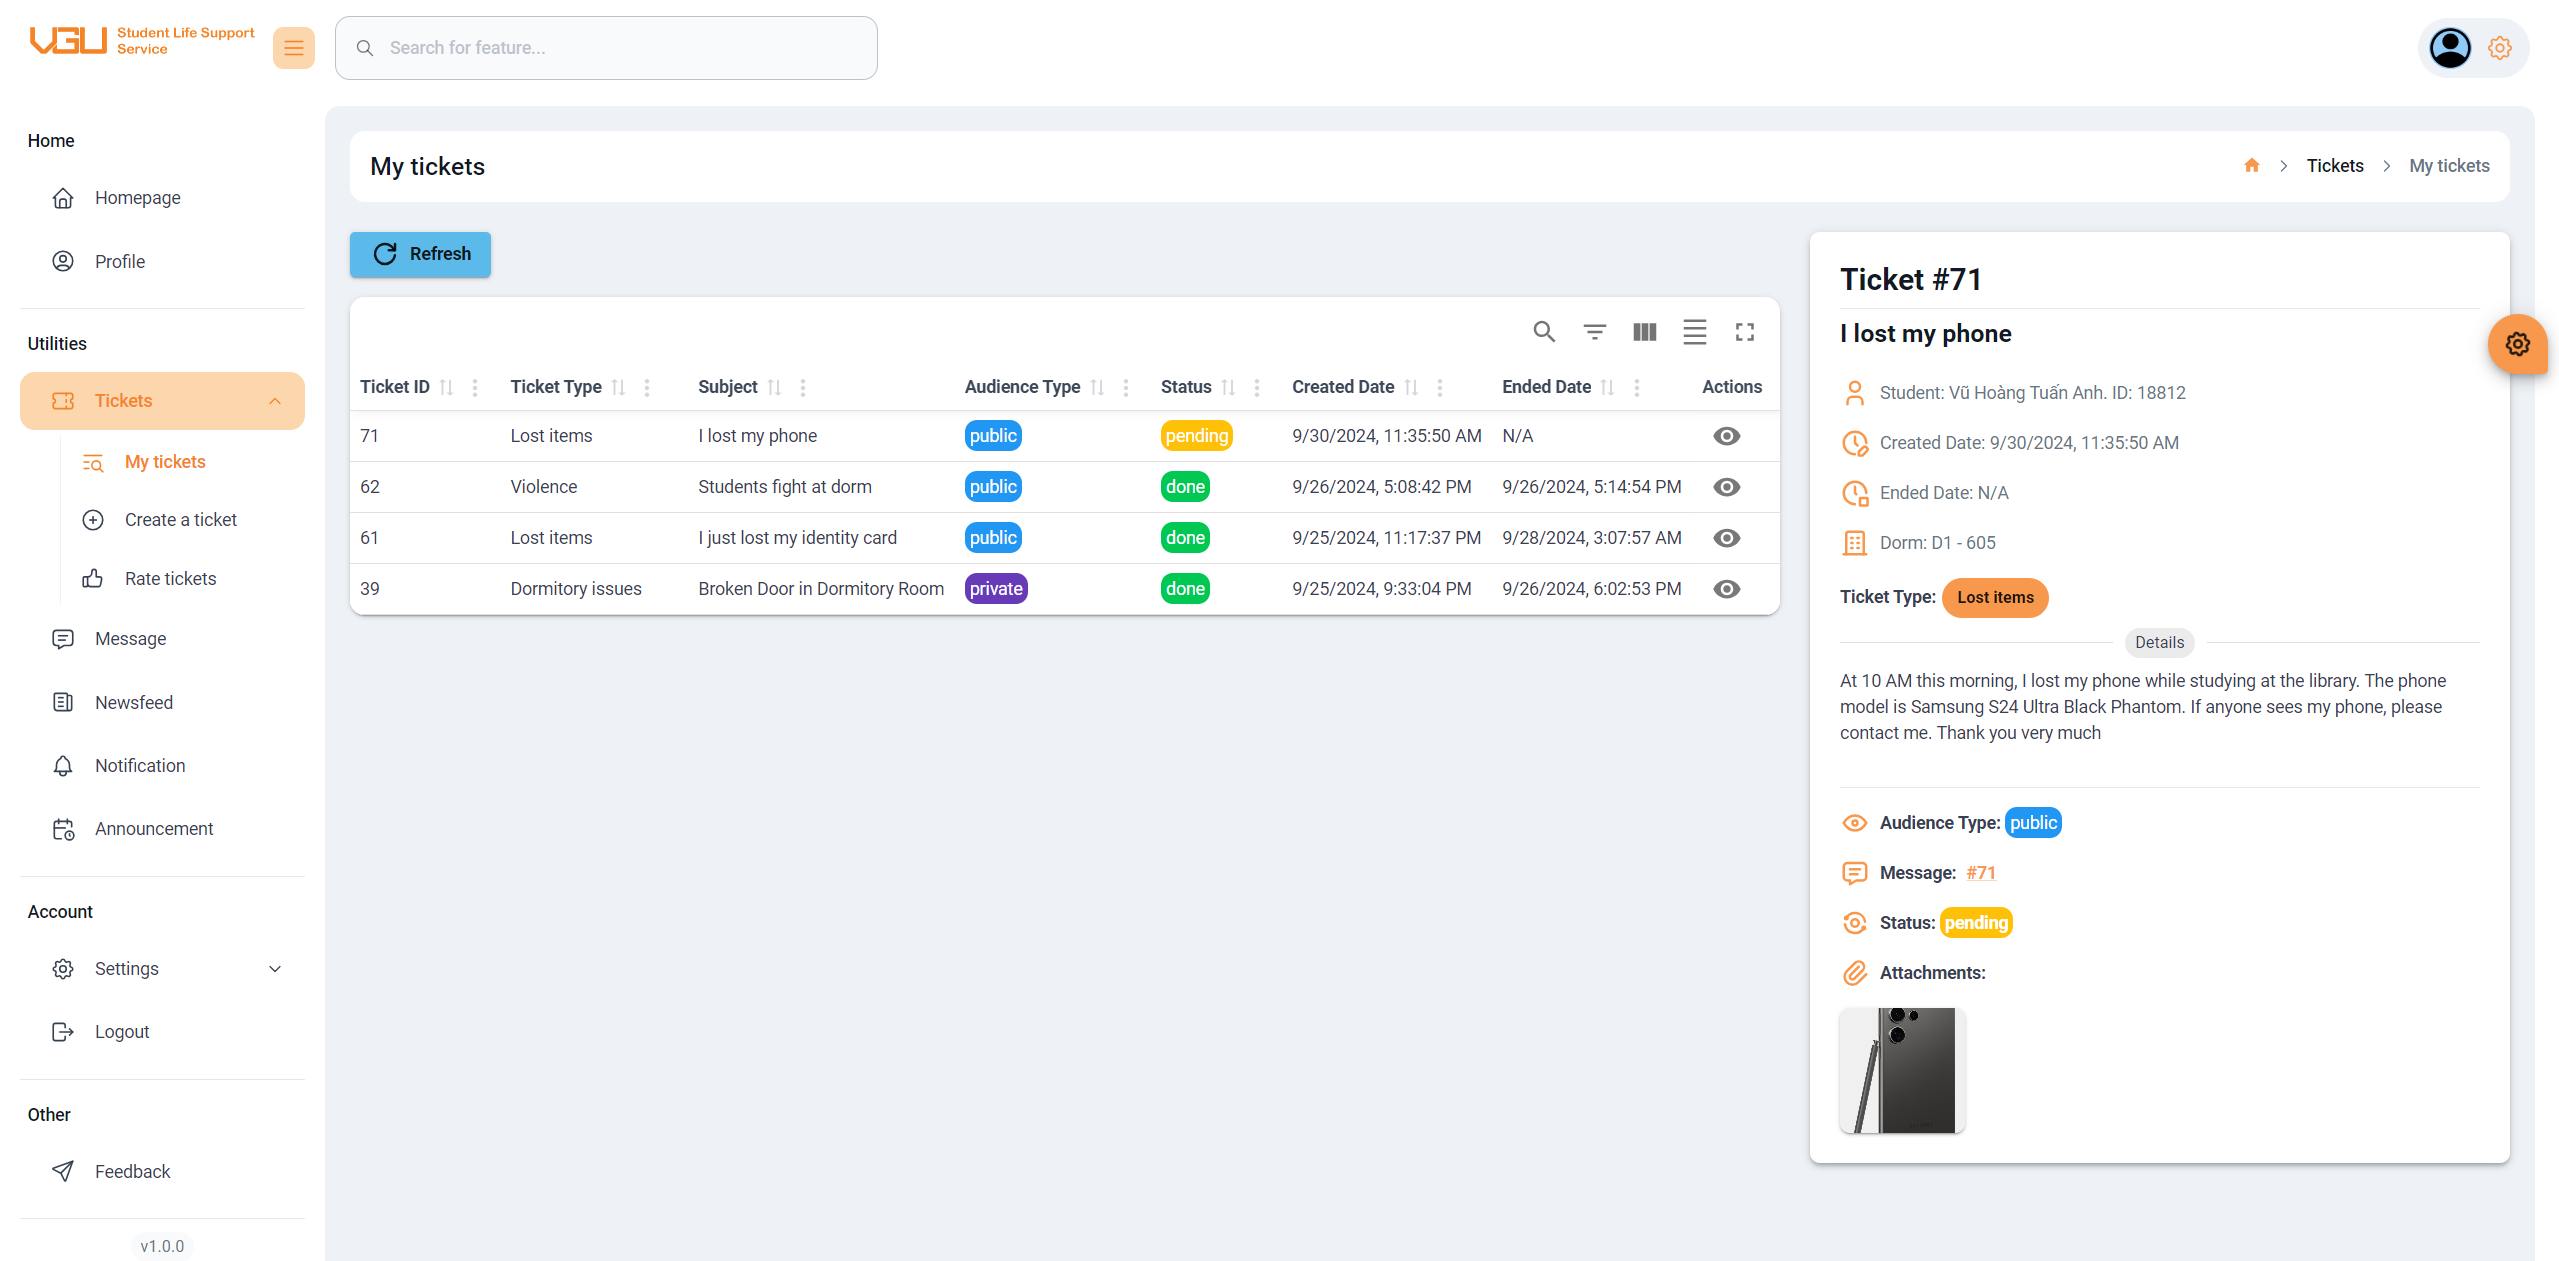
\includegraphics[width=1.0\linewidth]{graphics/gui/student/my-tickets}
		\caption{Student's Tickets List Page}
		\label{fig:gui-std-my-tickets}
	\end{figure}
	
	
	\subsubsection{Create Tickets}
	Students can submit a new support ticket by selecting \texttt{Tickets > Create a ticket}. After completing the form with all required information and clicking 'Create This Ticket', the ticket will be marked as pending, awaiting approval from an admin and resolution by the staff. (Figure \ref{fig:gui-std-create-ticket})
	
	\begin{figure}[H]
		\centering
		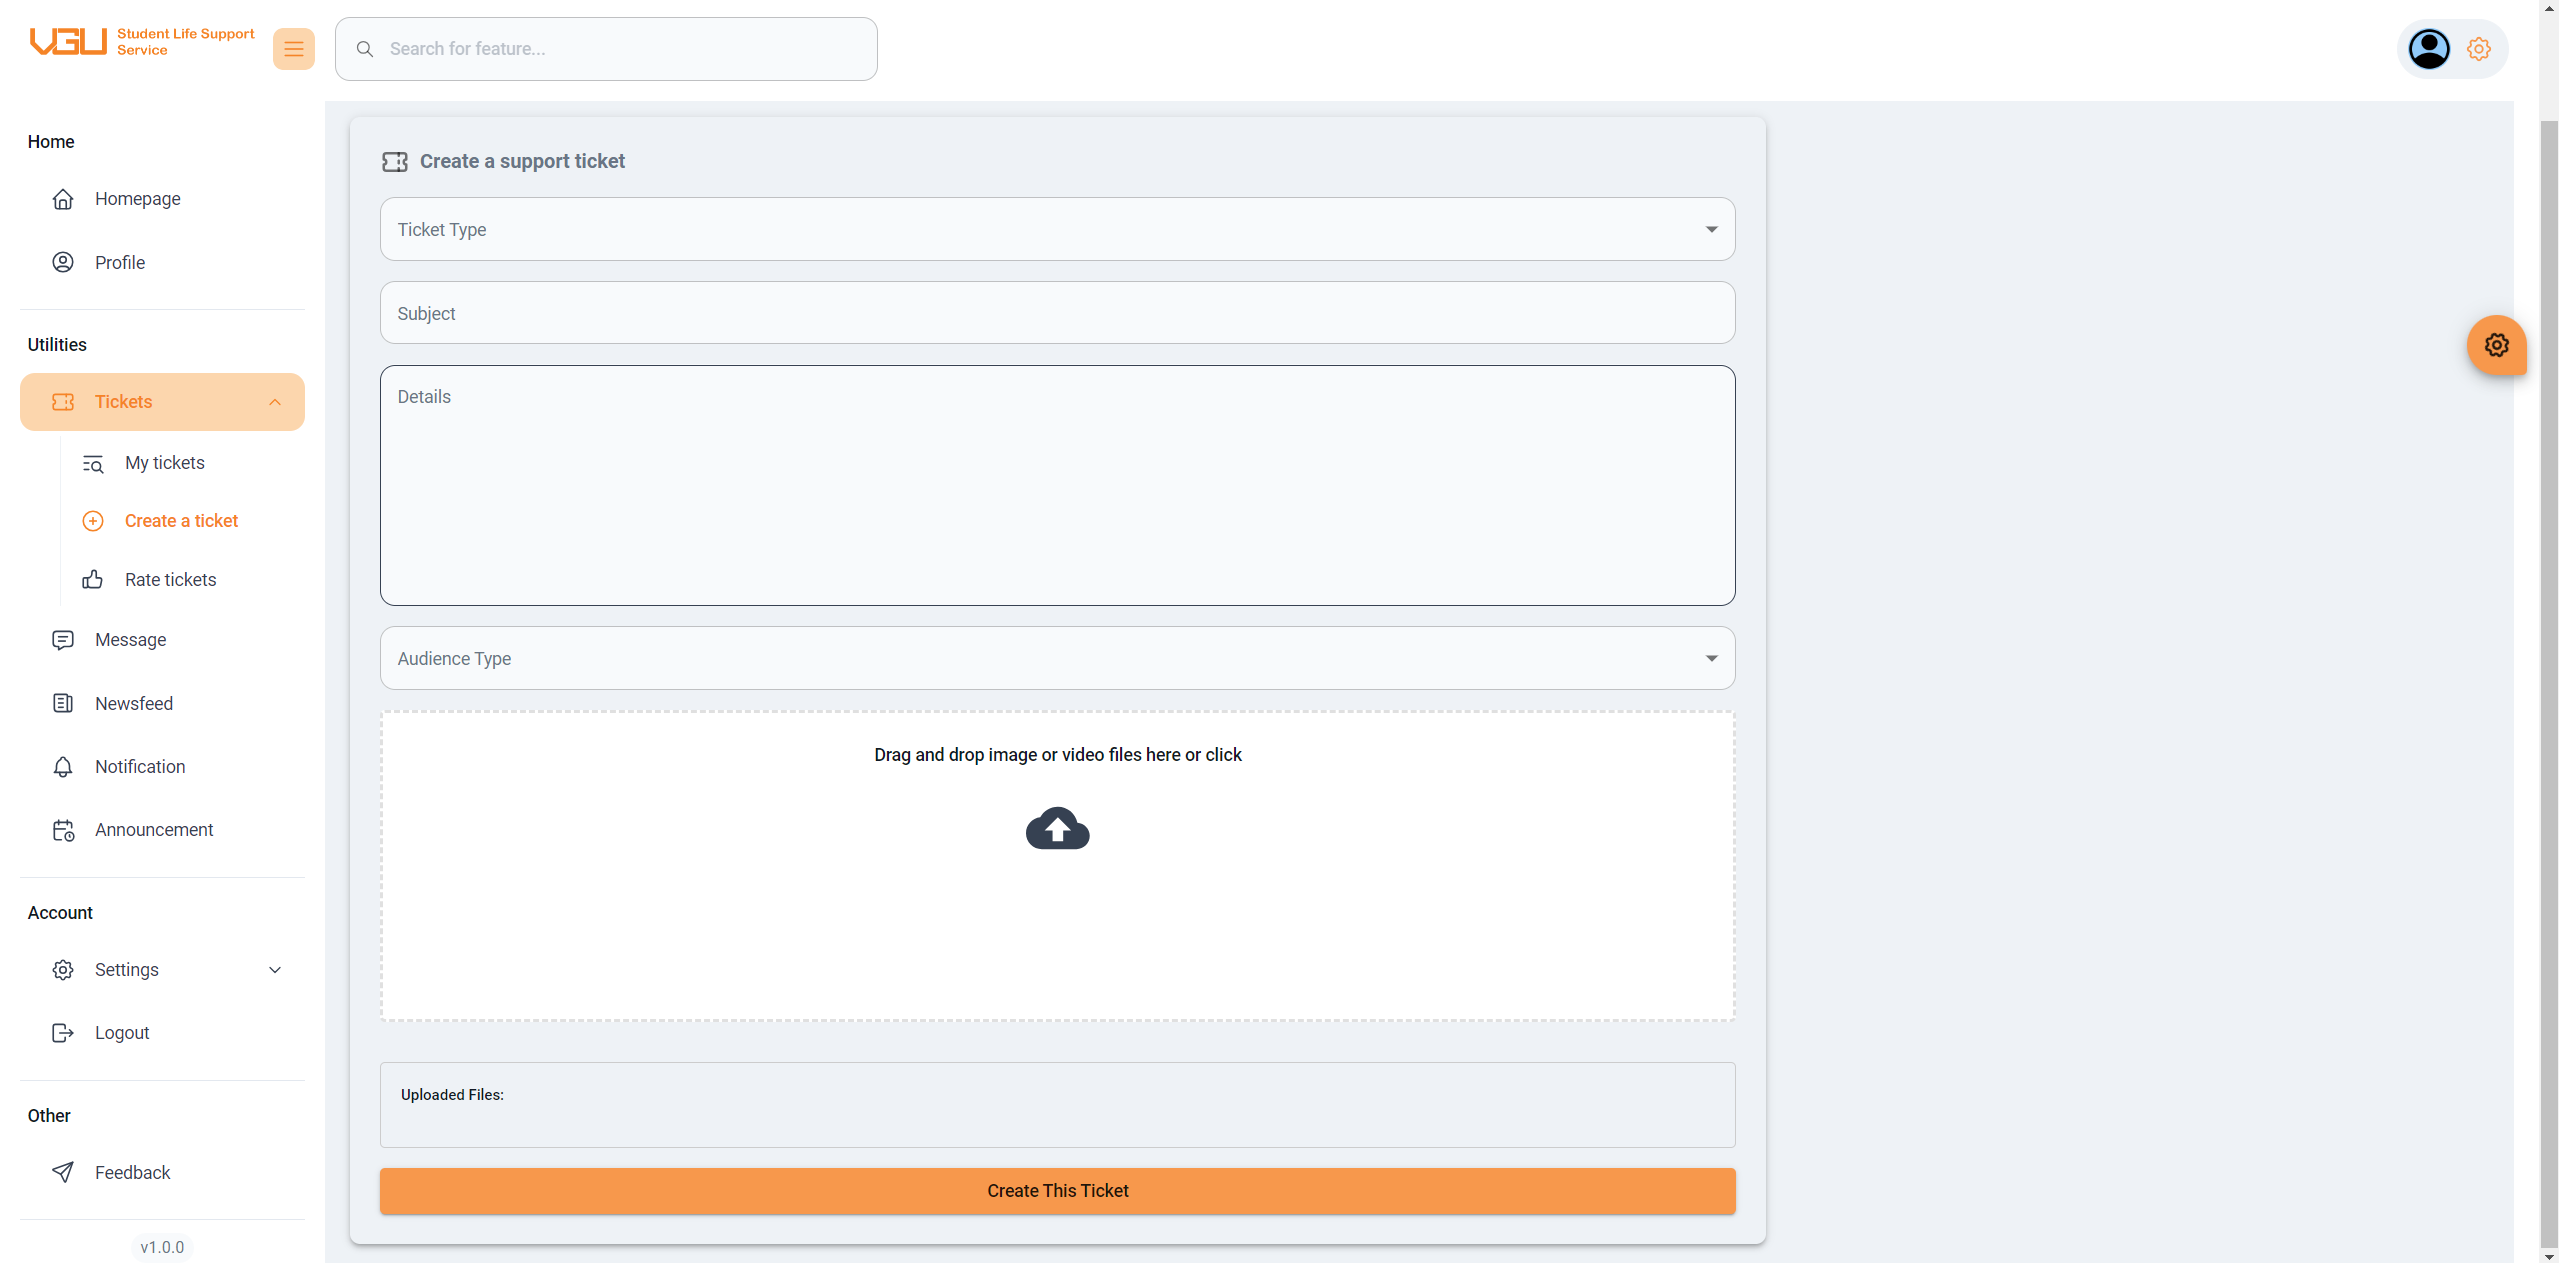
\includegraphics[width=1.0\linewidth]{graphics/gui/student/create-ticket}
		\caption{Student's Create Tickets Page}
		\label{fig:gui-std-create-ticket}
	\end{figure}
	
	
	\subsubsection{Rate Tickets}
	Once a ticket has been marked as completed, students have the option to provide feedback by rating the ticket through the "Rate Tickets" menu. To submit a rating, students can simply click the "Rate" action corresponding to each completed ticket and input their rating score before submitting it. (see Figures \ref{fig:gui-std-rate-ticket}, \ref{fig:gui-rate-ticket-modal})
	
	\begin{figure}[H]
		\centering
		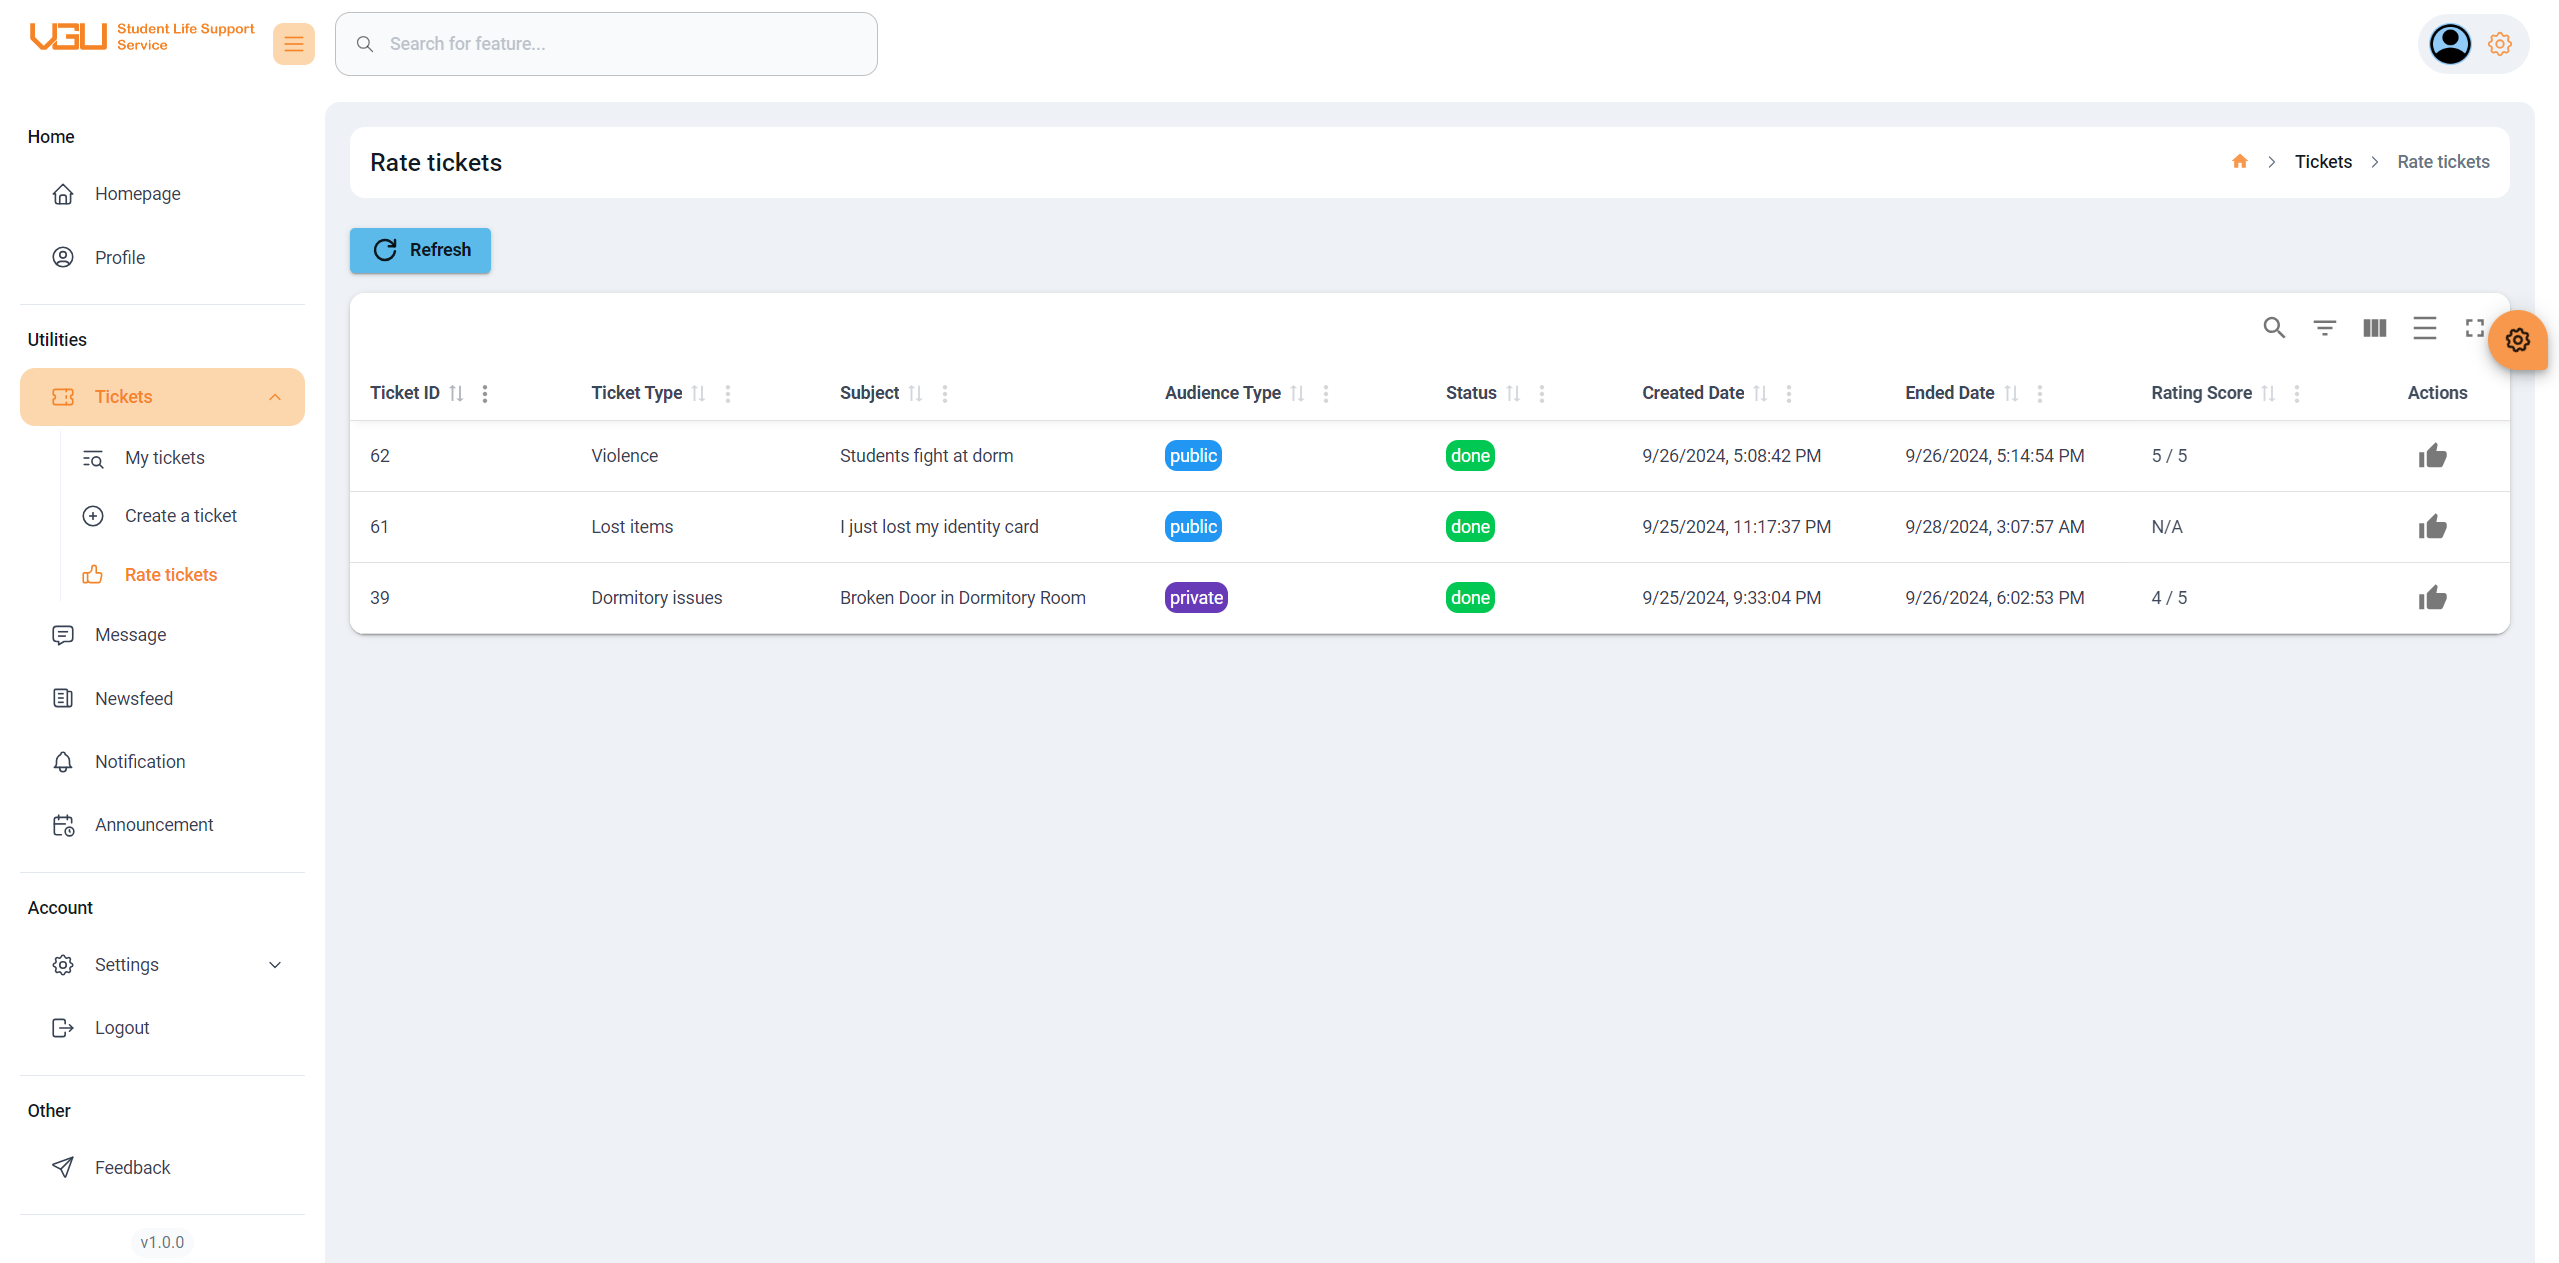
\includegraphics[width=1.0\linewidth]{graphics/gui/student/rate-ticket}
		\caption{Student's Rate Tickets Page}
		\label{fig:gui-std-rate-ticket}
	\end{figure}
	
	
	
	\begin{figure}[H]
		\centering
		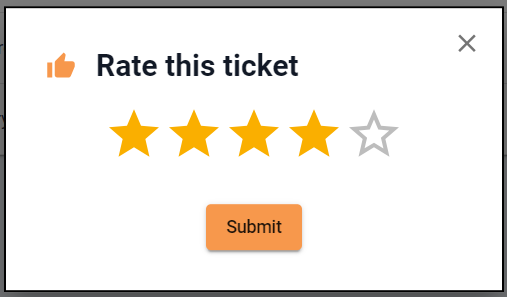
\includegraphics[width=0.5\linewidth]{graphics/gui/student/rate-ticket1}
		\caption{Submit a ticket rating}
		\label{fig:gui-rate-ticket-modal}
	\end{figure}
	
	
	
	\subsubsection{Message}

	\begin{figure}[H]
		\centering
		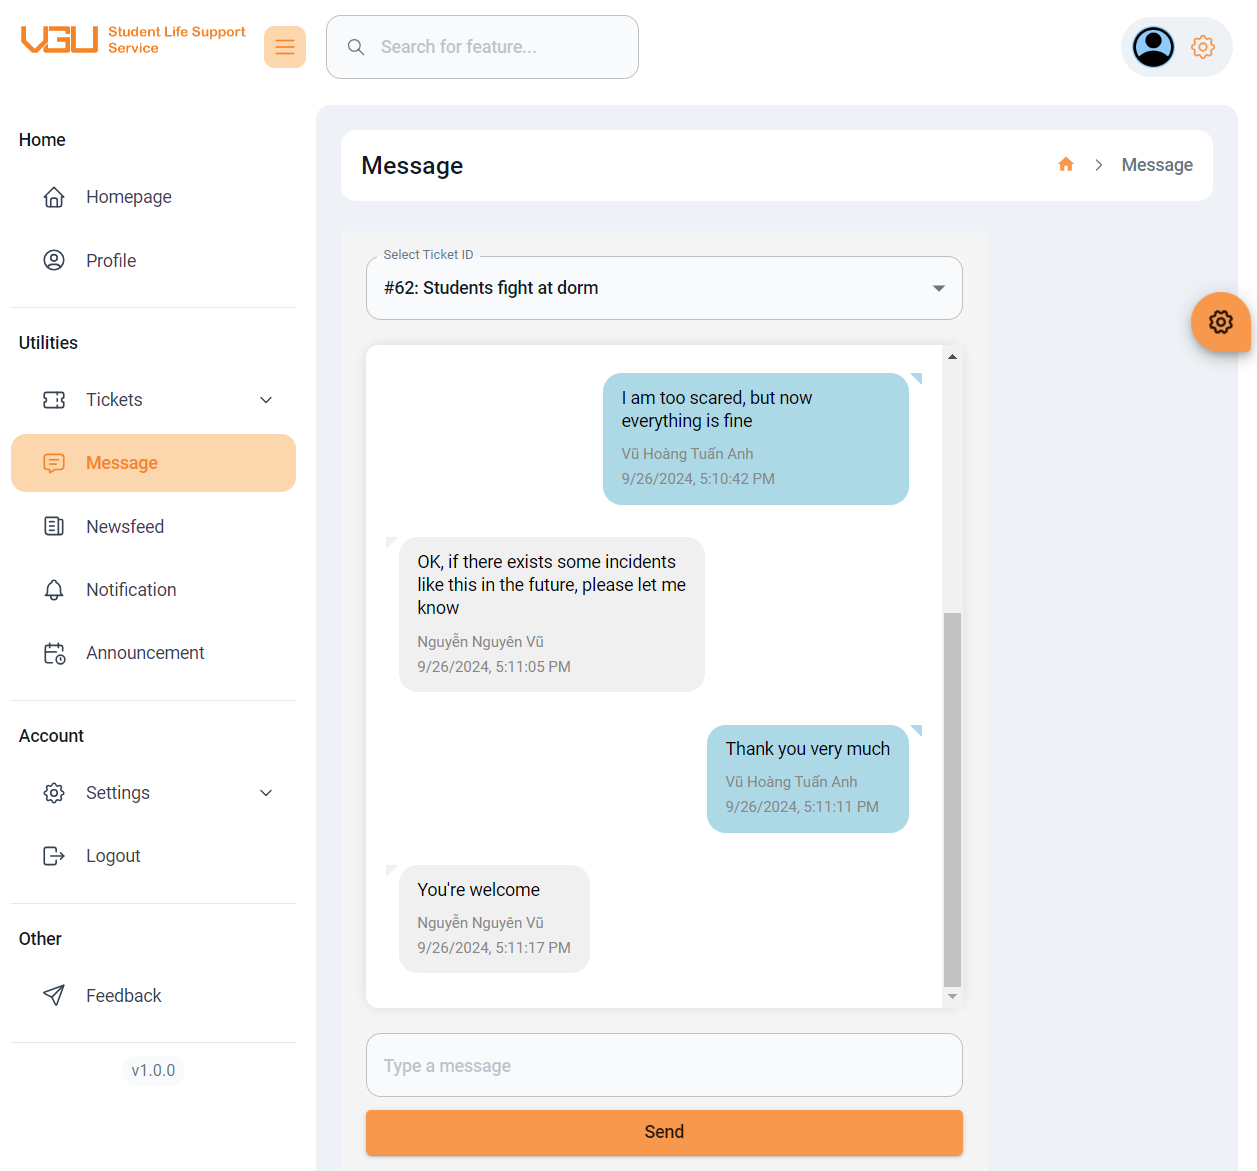
\includegraphics[width=0.9\linewidth]{graphics/gui/student/msg}
		\caption{Student's Message Page}
		\label{fig:gui-std-msg}
	\end{figure}
	Students can communicate with the staff assigned to their tickets by going to the "Message" menu. In this section, they can select the conversation associated with the ticket ID and send messages directly to the staff member handling their case. (Figure \ref{fig:gui-std-msg})
	

	
	
	
	\subsubsection{Newsfeed}
	\begin{figure}[H]
		\centering
		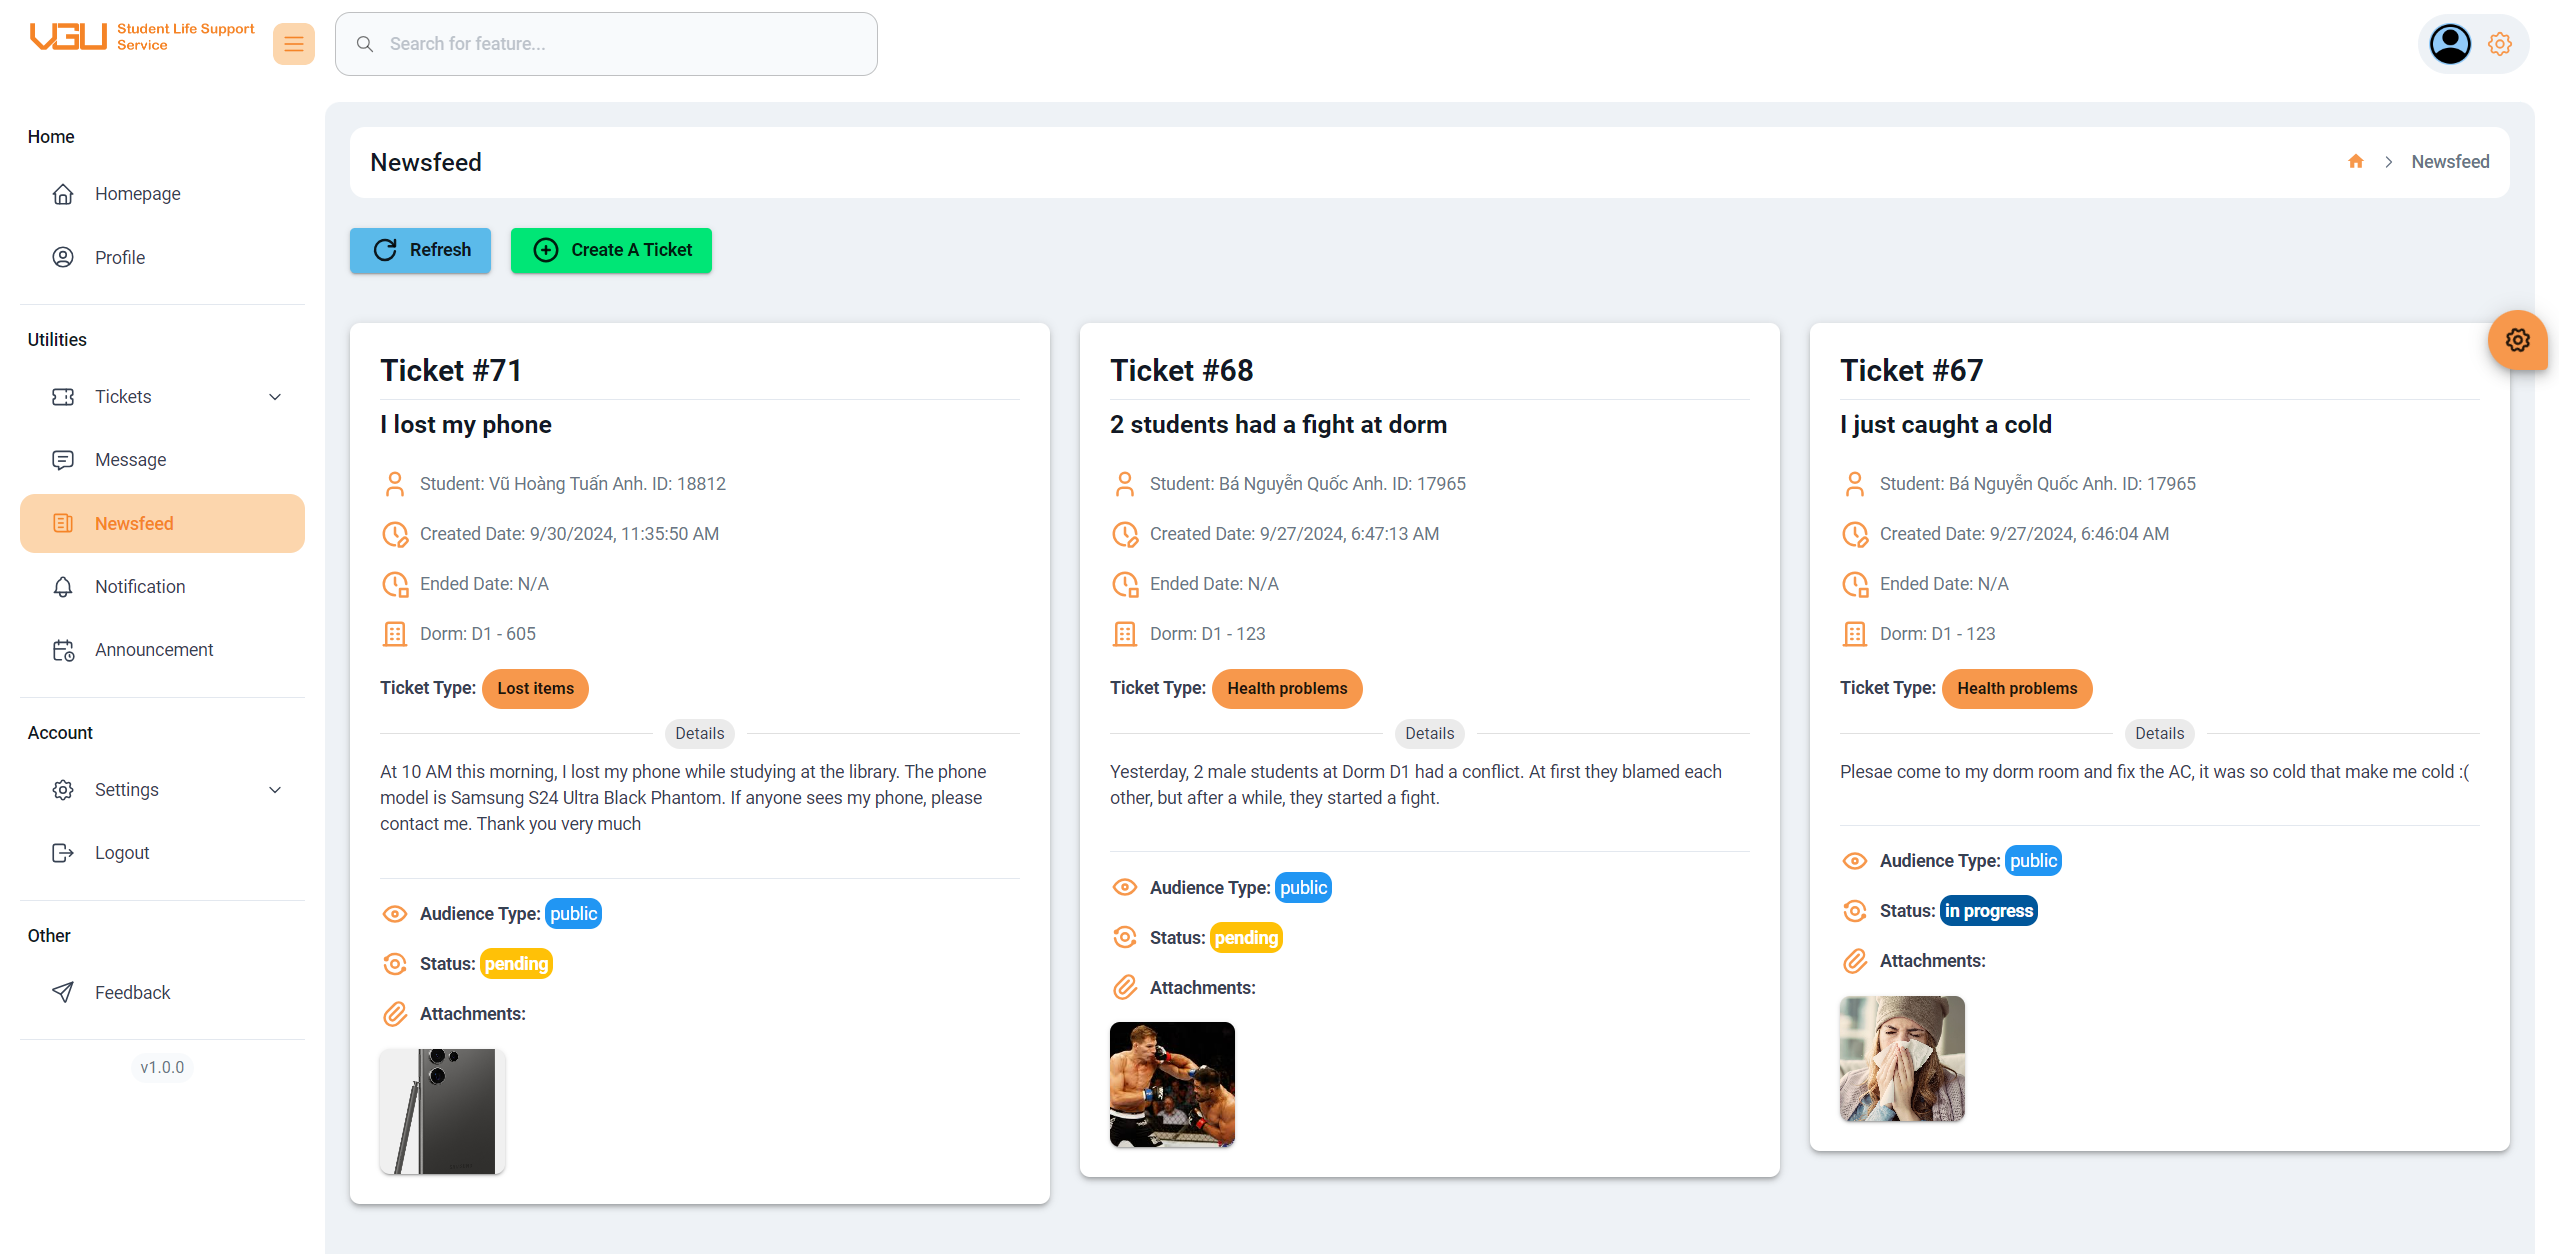
\includegraphics[width=1.0\linewidth]{graphics/gui/student/newsfeed}
		\caption{Student's Newsfeed}
		\label{fig:gui-std-newsfeed}
	\end{figure}
	
	Students have the ability to view public support tickets submitted by other students through the "News Feed" menu. This section provides access to a list of publicly shared tickets, allowing students to stay informed about common issues, solutions, or inquiries raised by their peers. (Figure \ref{fig:gui-std-newsfeed})
	
	
	
	\subsubsection{Notification}

	\begin{figure}[H]
		\centering
		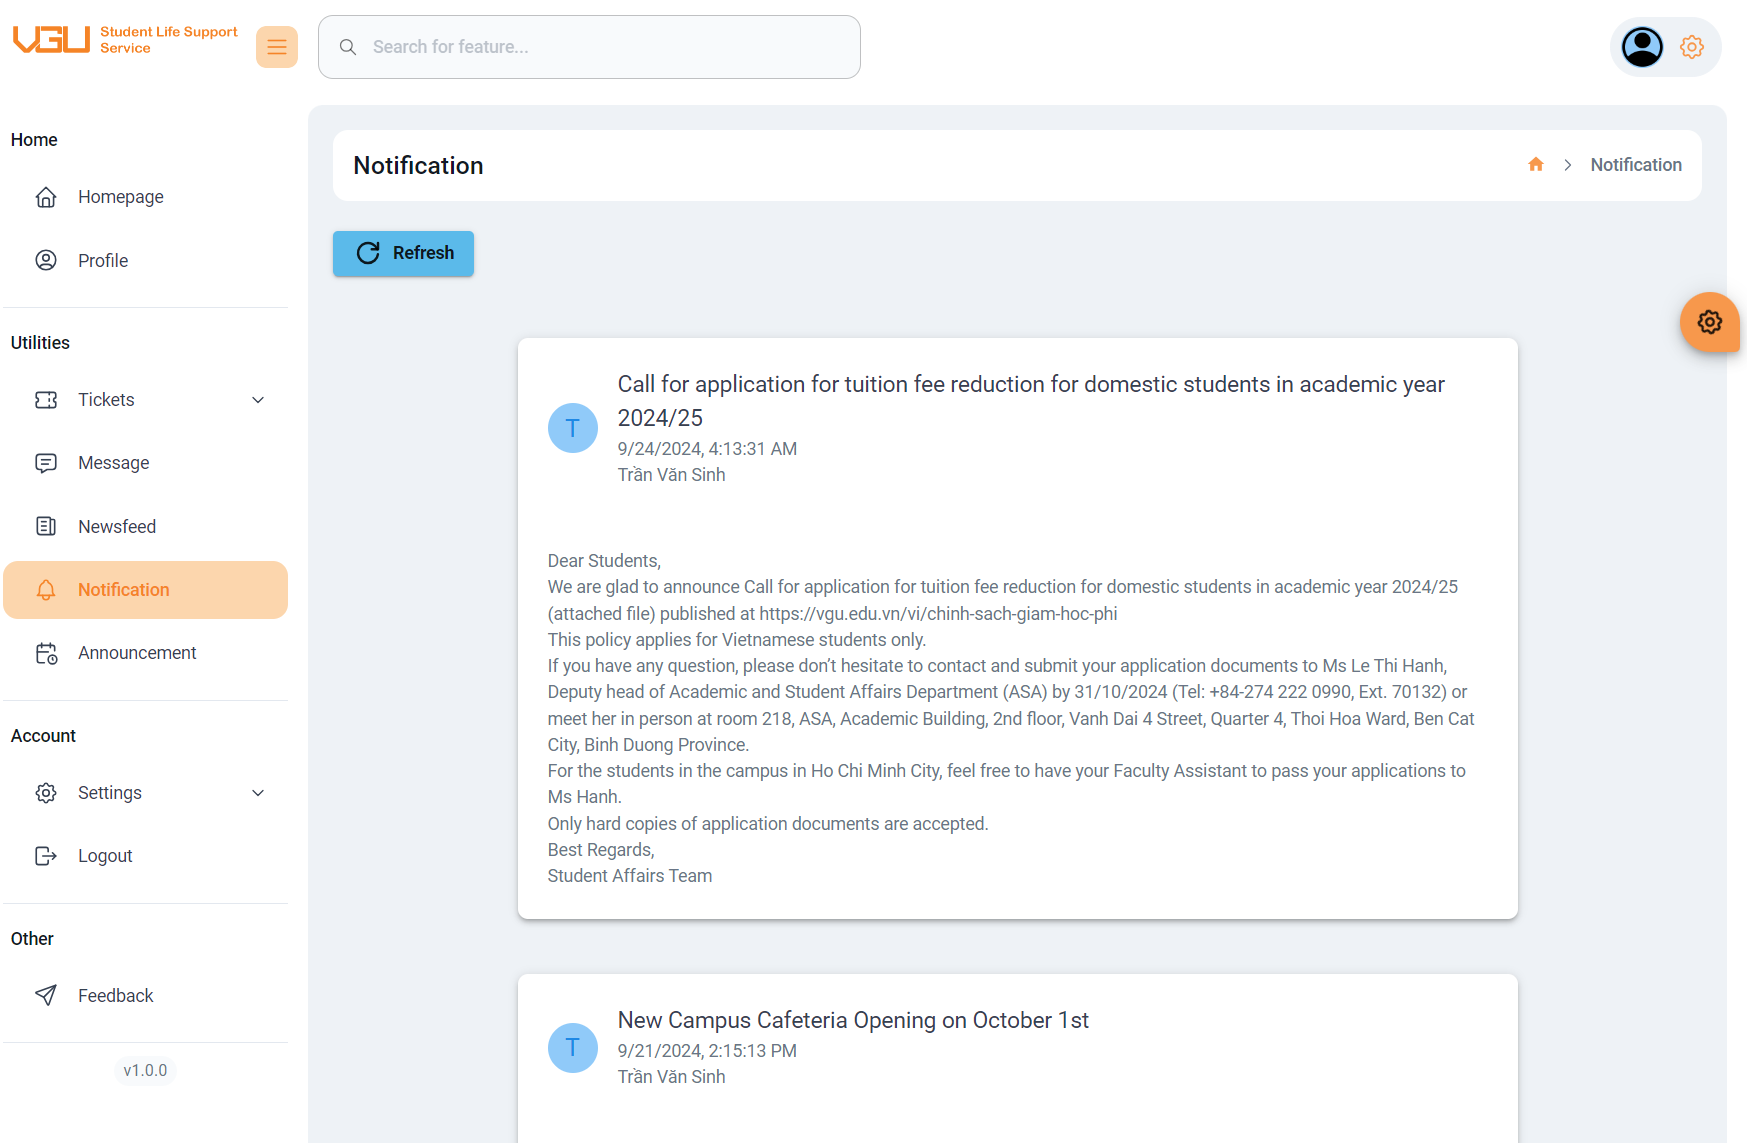
\includegraphics[width=1.0\linewidth]{graphics/gui/student/noti}
		\caption{Student's Notification Page}
		\label{fig:gui-std-noti}
	\end{figure}
		Students can receive important notifications from staff or administrators in the "Notification" menu. This section is dedicated to keeping students updated on various announcements, ticket status changes, or other critical communications from the support team. By regularly checking this menu, students ensure they stay informed about any new developments or actions that require their attention. Notifications may include updates on submitted tickets, administrative notices, or responses to queries. (Figure \ref{fig:gui-std-noti})
	
	
	
	\subsubsection{Announcement}
	\begin{figure}[H]
		\centering
		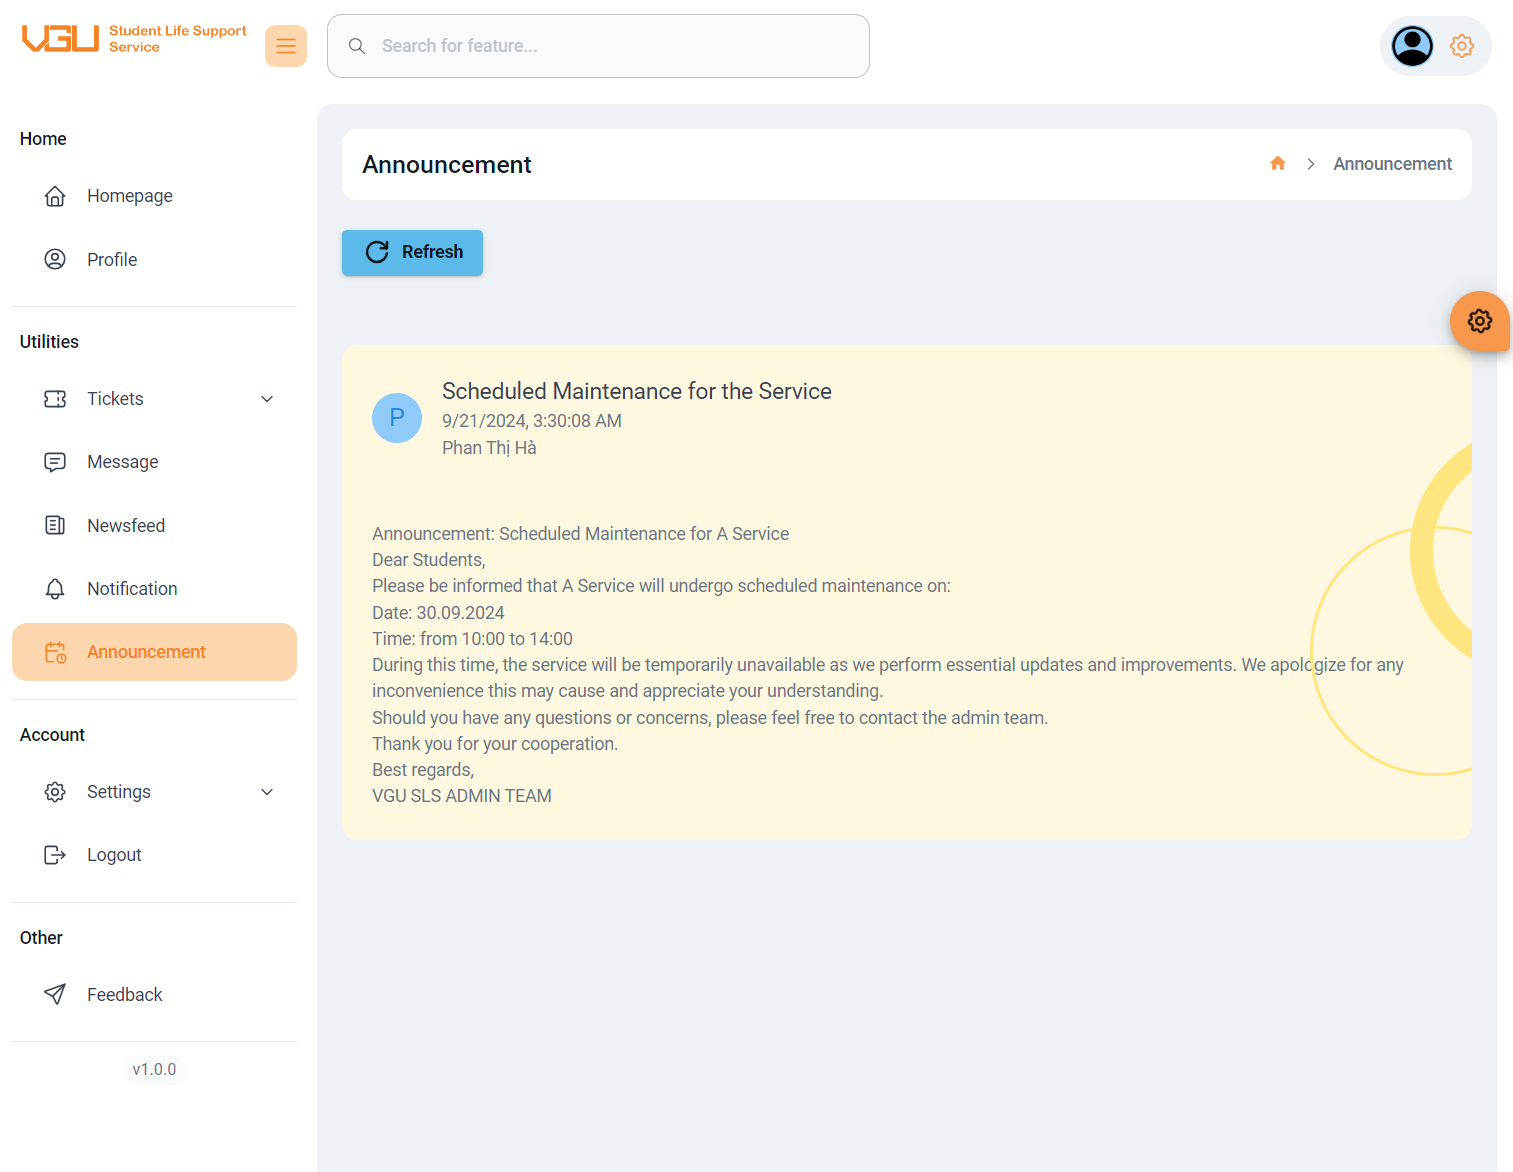
\includegraphics[width=1.0\linewidth]{graphics/gui/student/announcement}
		\caption{Student's Announcement Page}
		\label{fig:gui-std-announcement}
	\end{figure}
	
	Students can access important announcements from staff or administrators in the "Announcement" menu. This dedicated section provides students with updates and information relevant to their academic and campus life. By regularly checking the "Announcement" menu, students can stay informed about events, policy changes, or other significant news that may affect them. (Figure \ref{fig:gui-std-announcement})
	
	
	\subsubsection{Settings}
	Students have the ability to modify their personal information and change their account password through the "Settings" menu. This feature allows students to ensure that their details are up to date, which is crucial for effective communication and account security. By navigating to the "Settings" menu, students can easily access fields to edit their name, contact information, and other relevant details. Additionally, they can update their password to enhance their account's security, ensuring that their personal data remains protected. This functionality empowers students to take control of their profiles and maintain accurate and secure information.
	
	\begin{figure}[H]
		\centering
		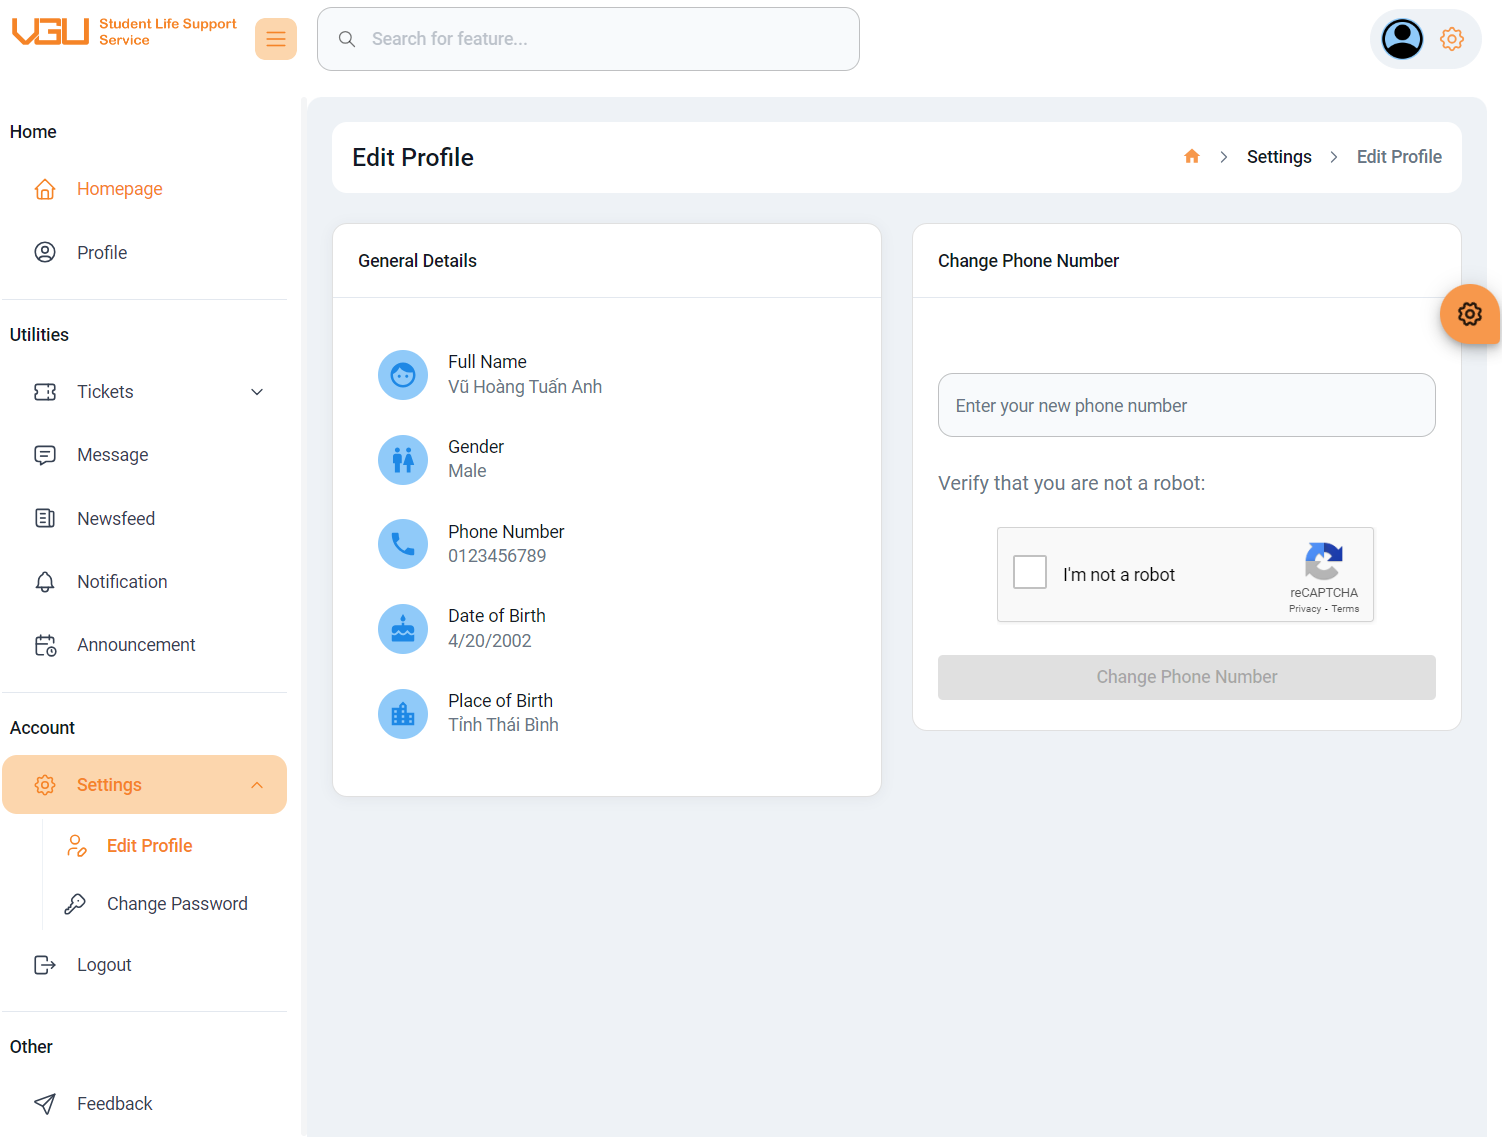
\includegraphics[width=1.0\linewidth]{graphics/gui/student/sett-edit-profile}
		\caption{Student's Edit Profile Page}
		\label{fig:gui-std-sett-edit-profile}
	\end{figure}
	
	
	\begin{figure}[H]
		\centering
		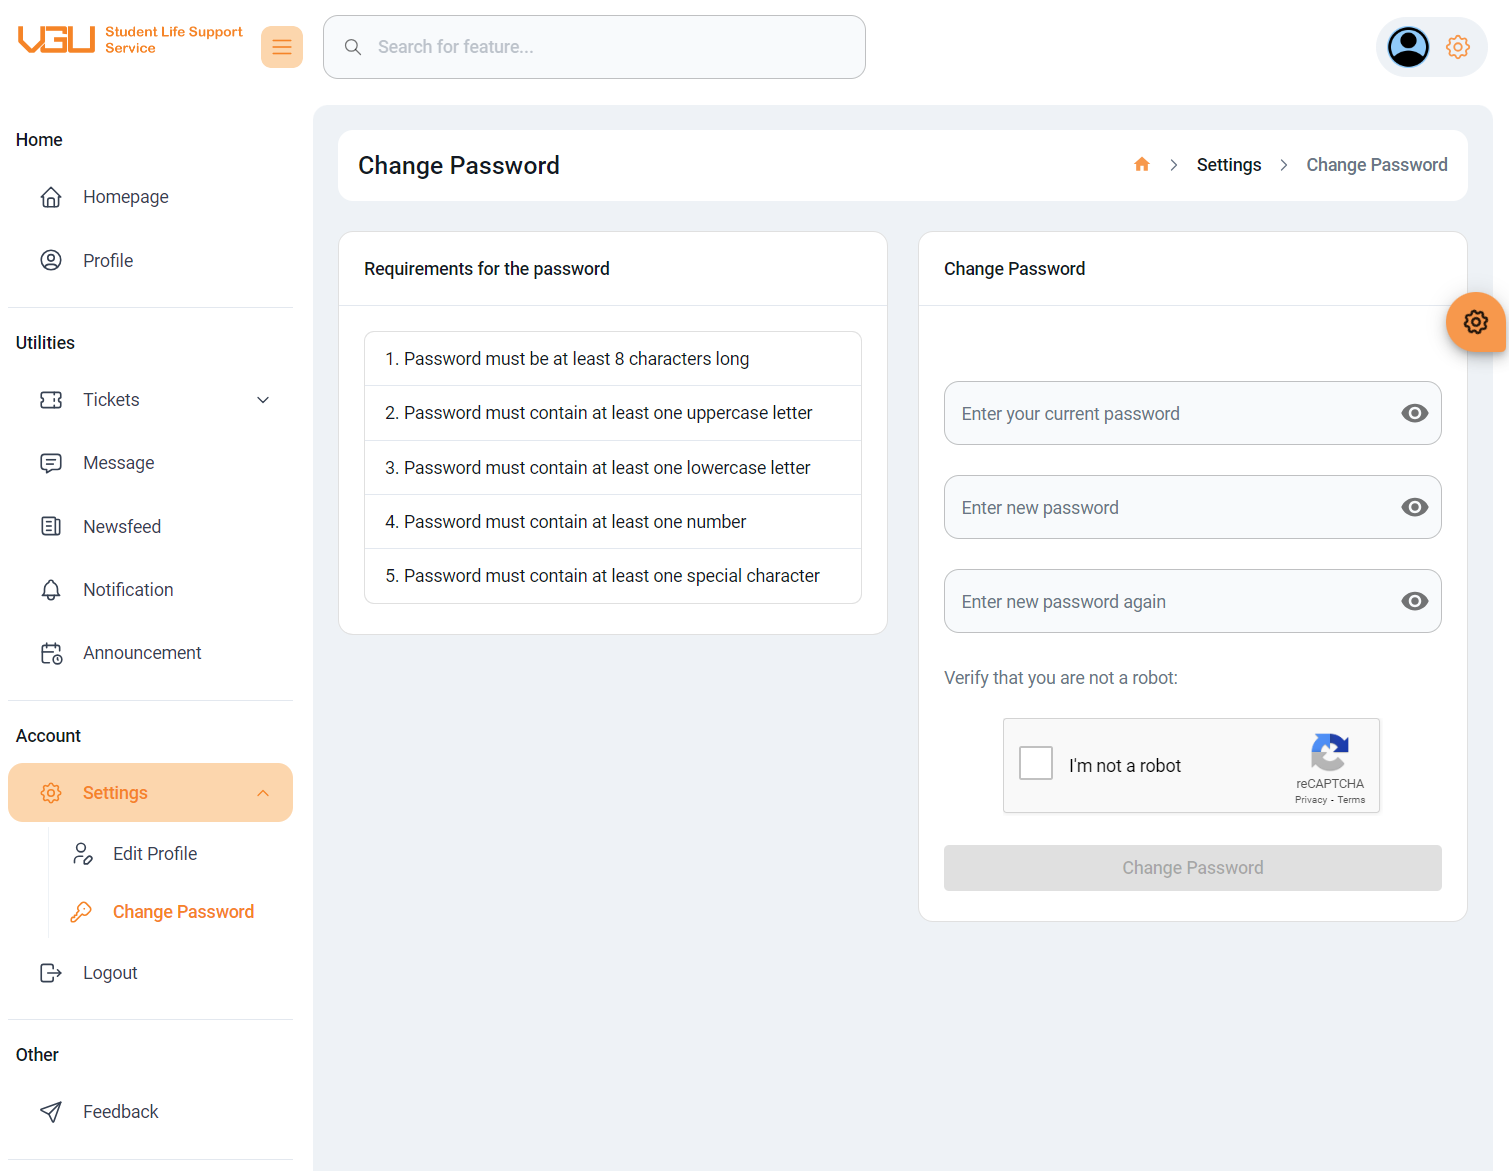
\includegraphics[width=1.0\linewidth]{graphics/gui/student/sett-password}
		\caption{Student's Change Password Page}
		\label{fig:gui-std-sett-password}
	\end{figure}
	
	
	\subsubsection{Feedback}
	Students have the opportunity to provide feedback on the system by accessing the "Feedback" menu. Within this section, they can express their thoughts and experiences regarding the platform, which is essential for continuous improvement and user satisfaction. Additionally, students are encouraged to rate their experience by selecting a rating score before submitting their feedback. This structured approach allows them to convey not only qualitative insights but also quantitative assessments, enabling the administrators to better understand user satisfaction and identify areas that may require enhancements. By engaging in this feedback process, students contribute to the overall development and effectiveness of the system. (see Figure \ref{fig:gui-std-feedback})
	\begin{figure}[H]
		\centering
		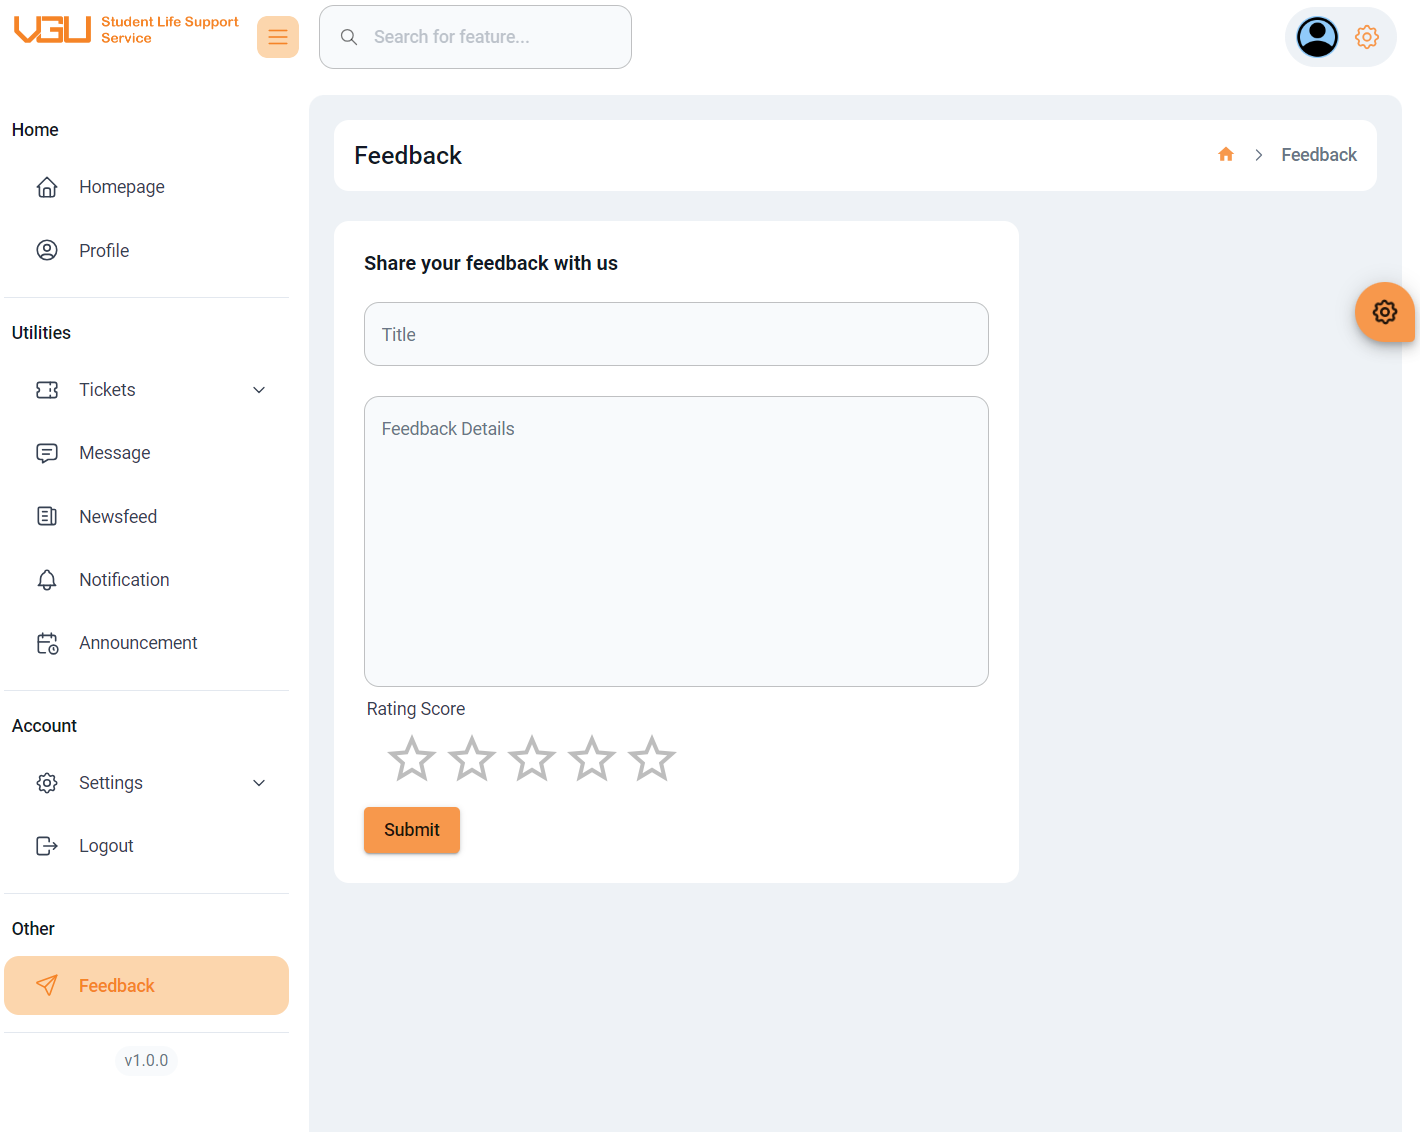
\includegraphics[width=1.0\linewidth]{graphics/gui/student/feedback}
		\caption{Student's Feedback Page}
		\label{fig:gui-std-feedback}
	\end{figure}
	
	
\subsection{Staff's functions}

	\subsubsection{Available Tickets}
		Staff members have access to the "Available Tickets" menu, where they can view a comprehensive list of all pending tickets. This menu serves as a centralized hub for managing incoming requests from students, allowing staff to efficiently monitor and address each ticket's status. Once they navigate to this section, staff can review the details of each pending ticket, including the nature of the issue raised by the student. From there, they can take appropriate actions to resolve the issues, whether that involves communicating with the student for further clarification, assigning the ticket to the relevant department, or providing direct assistance. This streamlined process ensures that all student inquiries are handled promptly and effectively, contributing to a more responsive support system.
		
	\begin{figure}[H]
		\centering
		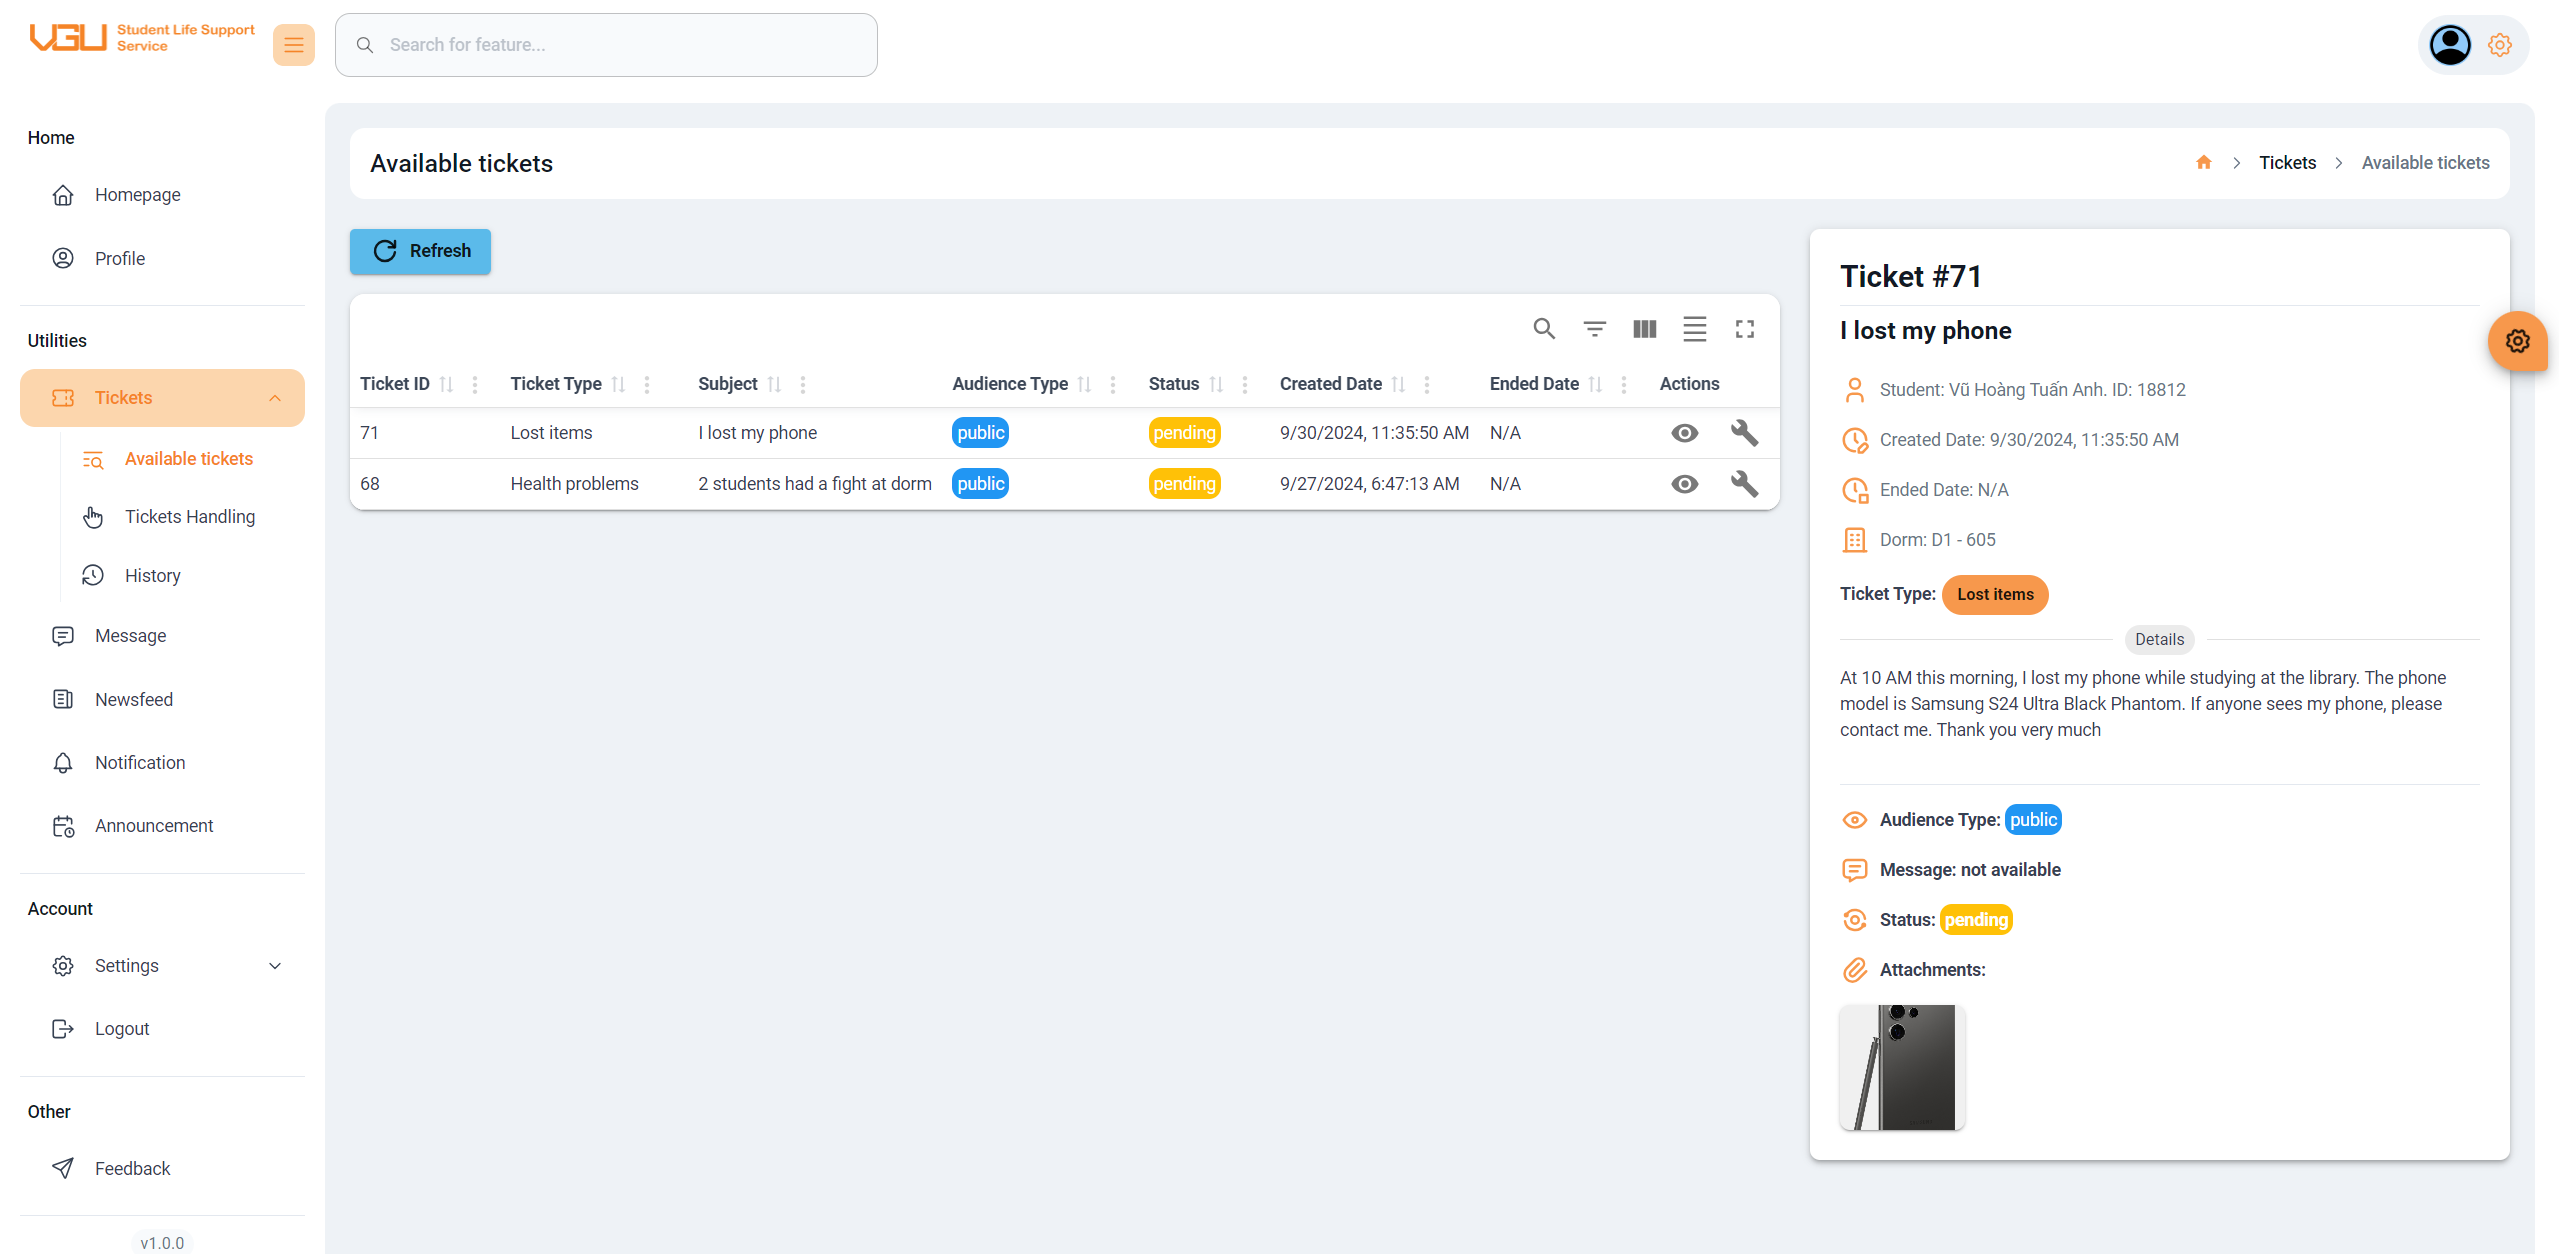
\includegraphics[width=1\linewidth]{graphics/gui/staff/avail-ticket}
		\caption{Staff's Available Tickets Page}
		\label{fig:gui-st-avail-ticket}
	\end{figure}
	

	
	\begin{figure}[H]
		\centering
		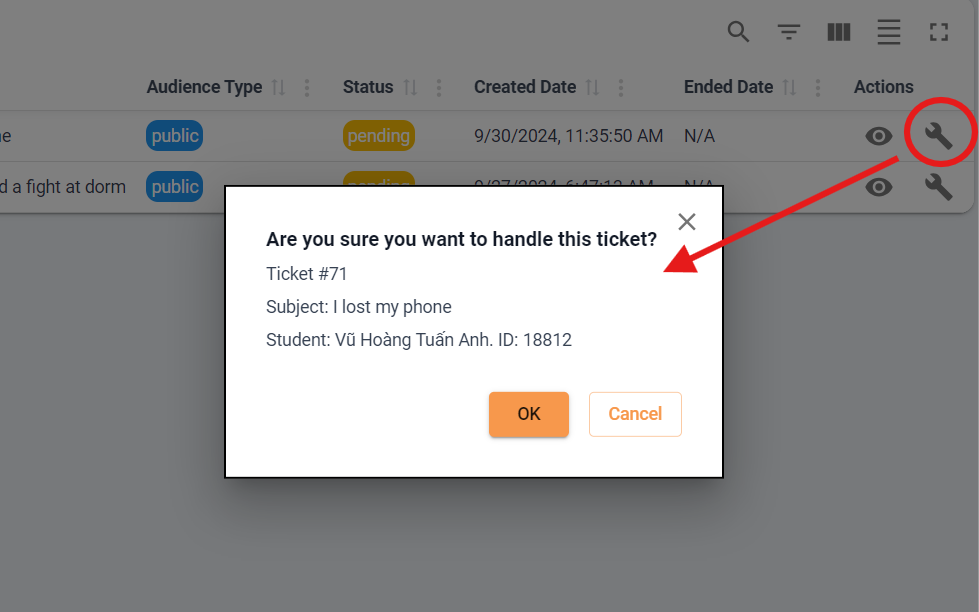
\includegraphics[width=0.8\linewidth]{graphics/gui/staff/avail-ticket-handle}
		\caption{Handle a ticket}
		\label{fig:gui-st-avail-ticket-handle}
	\end{figure}
	
	
	\begin{figure}[H]
		\centering
		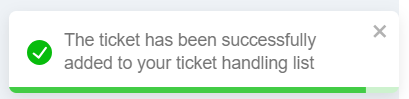
\includegraphics[width=0.5\linewidth]{graphics/gui/staff/avail-ticket-handle-success}
		\caption{Successfully add a ticket to ticket handling list}
		\label{fig:gui-st-avail-ticket-handle-success}
	\end{figure}
	
	
	\subsubsection{Tickets Handling}
	Within the "Ticket Handling" menu, staff members have the ability to manage tickets efficiently by marking them as completed or canceling them as necessary. This menu provides a dedicated interface for staff to oversee the progress of each ticket. When a ticket is resolved to the satisfaction of the student or when the issue has been adequately addressed, staff can easily mark it as "done." This action not only updates the ticket's status in the system but also informs the student that their request has been successfully fulfilled. Alternatively, if a ticket needs to be canceled—perhaps due to a change in the student's needs or if the issue is no longer relevant—staff can take this action as well. By allowing for these functionalities, the Ticket Handling menu plays a crucial role in maintaining clear communication between staff and students while ensuring that all ticket statuses are accurately reflected in the system.
	\begin{figure}[H]
		\centering
		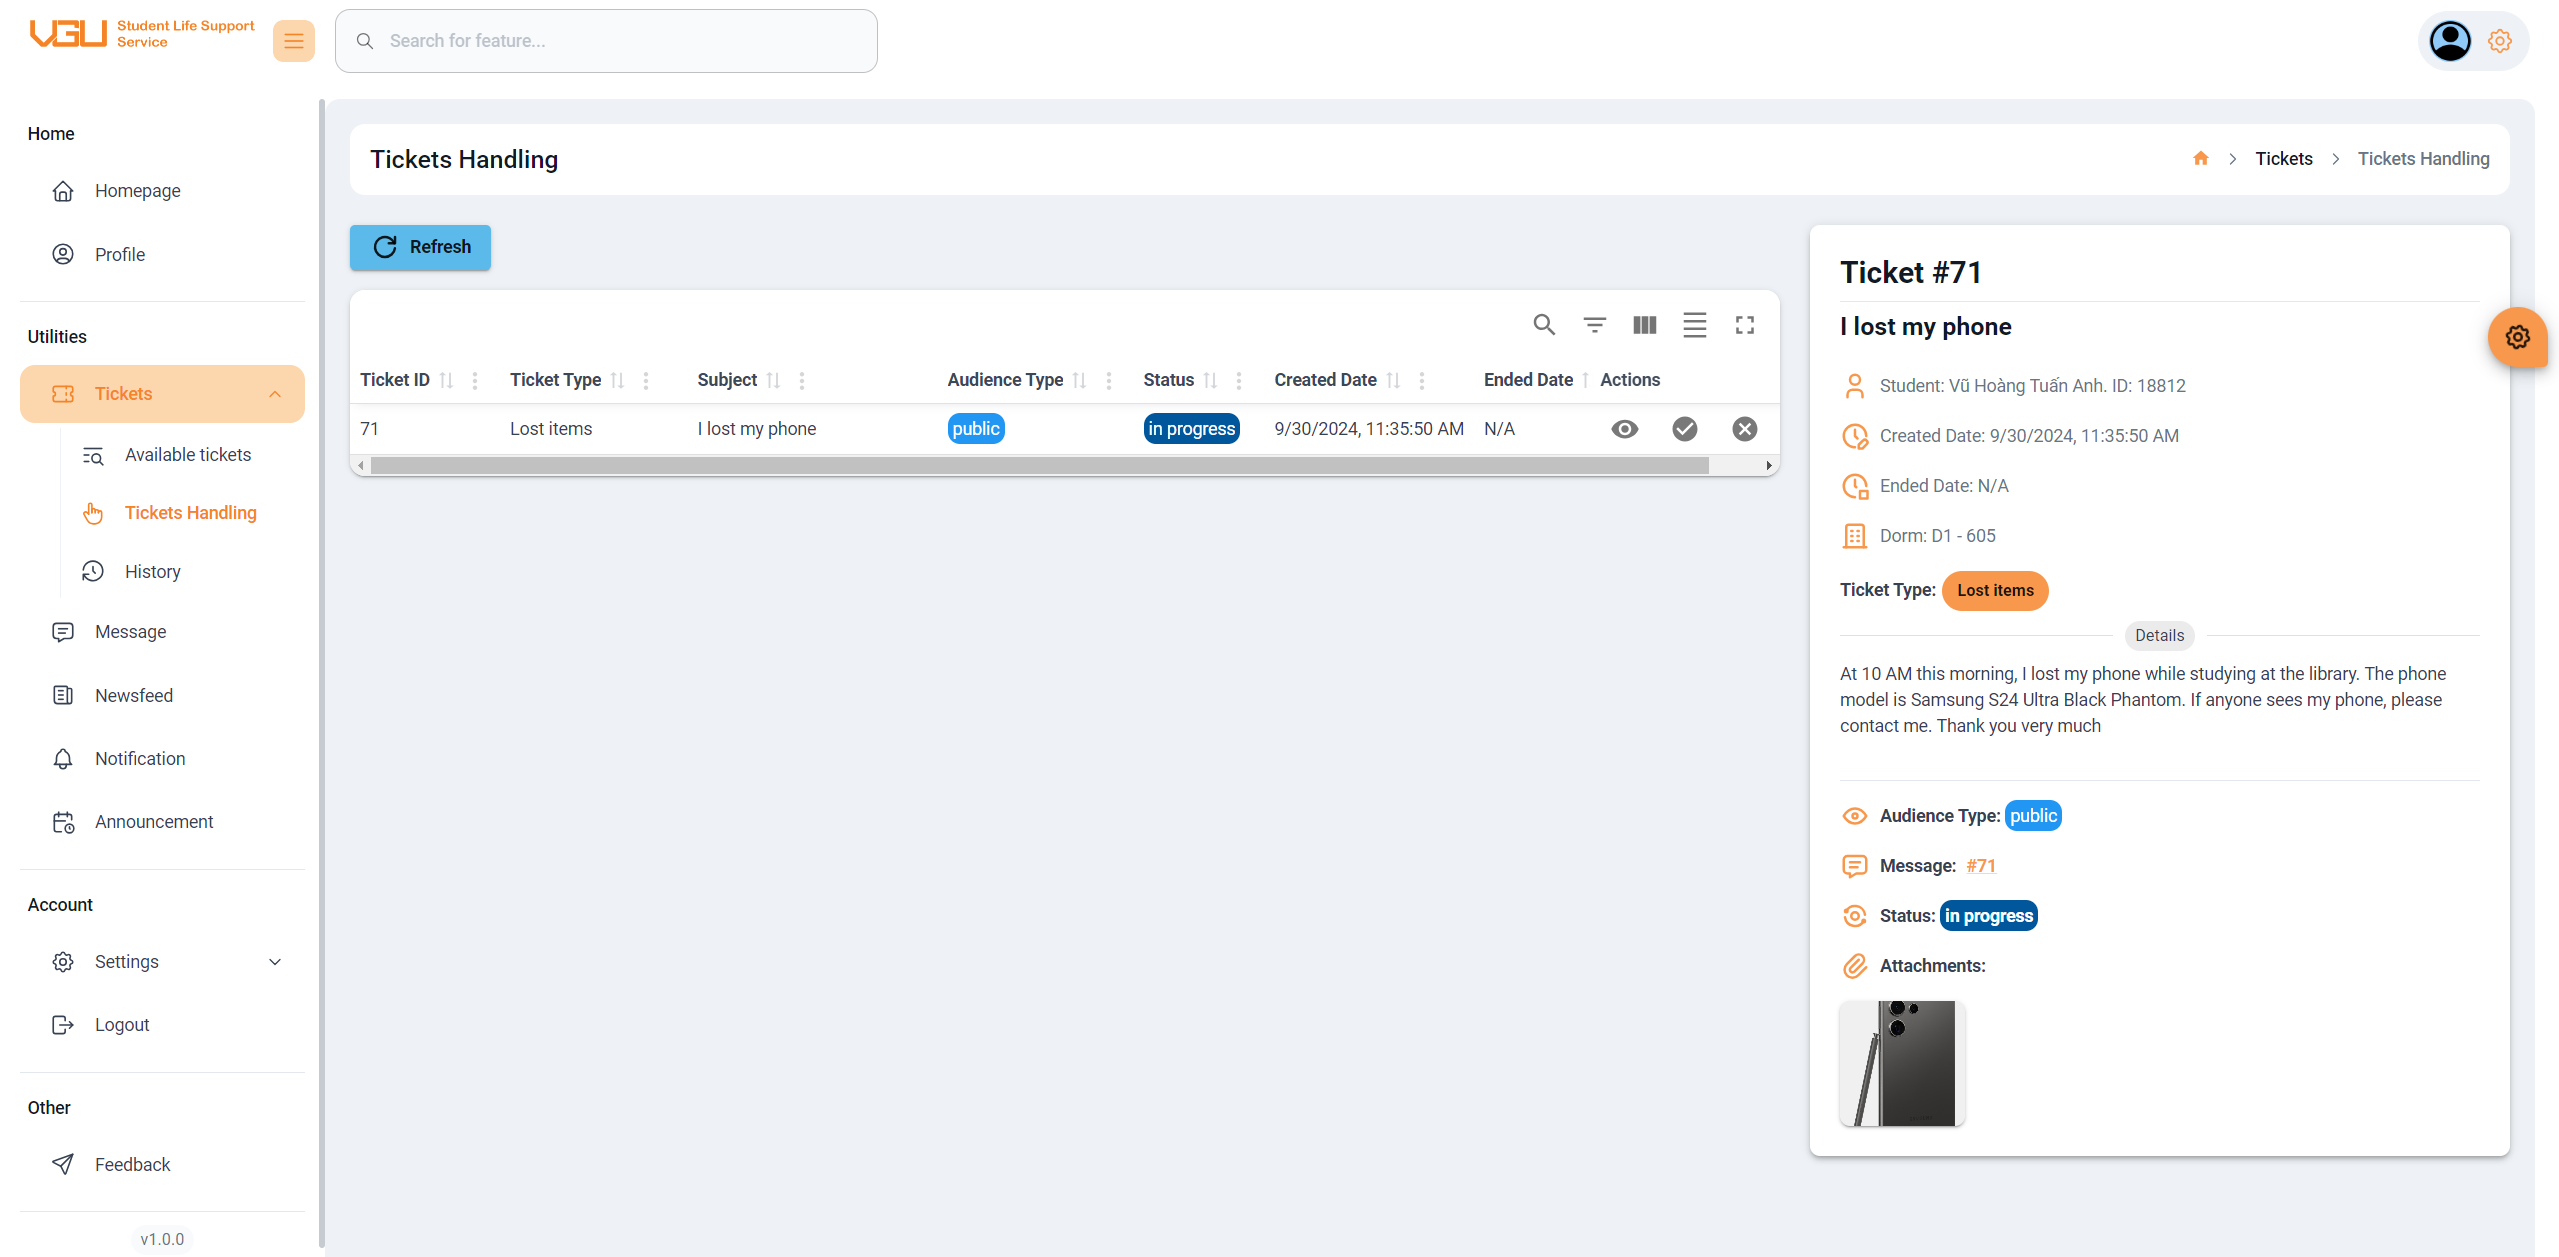
\includegraphics[width=1\linewidth]{graphics/gui/staff/ticket-handling}
		\caption{Staff's Tickets Handling List}
		\label{fig:gui-st-ticket-handling}
	\end{figure}
	
	
	\begin{figure}[H]
		\centering
		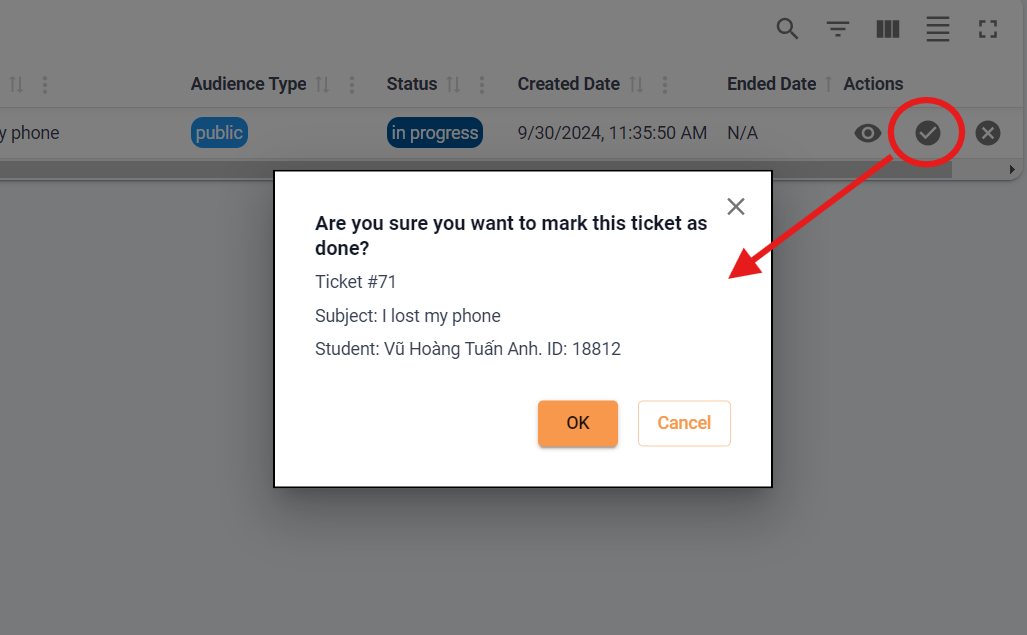
\includegraphics[width=0.7\linewidth]{graphics/gui/staff/ticket-handling-done}
		\caption{Mark a ticket as done}
		\label{fig:gui-st-ticket-handling-done}
	\end{figure}
	
	\begin{figure}[H]
		\centering
		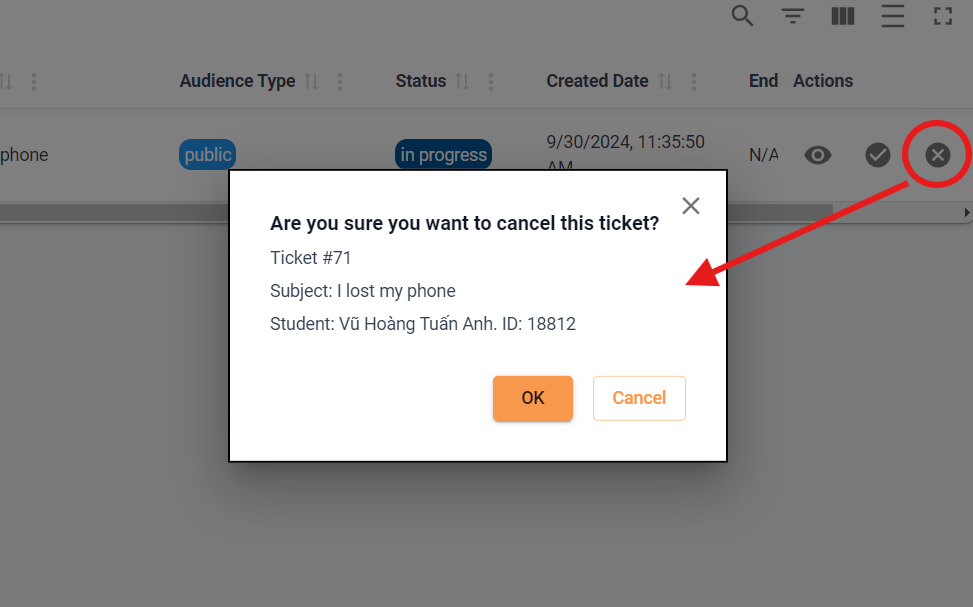
\includegraphics[width=0.7\linewidth]{graphics/gui/staff/ticket-handling-cancel}
		\caption{Cancel a ticket}
		\label{fig:gui-st-ticket-handling-cancel}
	\end{figure}
	
	
	
	
	\subsubsection{Tickets History}
	
	Staff members have the capability to access a comprehensive record of all past tickets through the "Tickets History" section. This feature allows them to review and analyze previously handled tickets, providing valuable insights into the nature of the inquiries and issues raised by students. In the Tickets History, staff can examine the details of each ticket, including the submission date, resolution status, and any notes or comments that were recorded during the handling process. This historical data is essential for assessing the effectiveness of past responses, identifying recurring issues, and improving the overall support process. By utilizing the information available in the Tickets History, staff can enhance their understanding of student concerns and refine their approach to future ticket management, ultimately leading to a more efficient and responsive support system. (see Figure \ref{fig:gui-st-ticket-history})
	\begin{figure}[H]
		\centering
		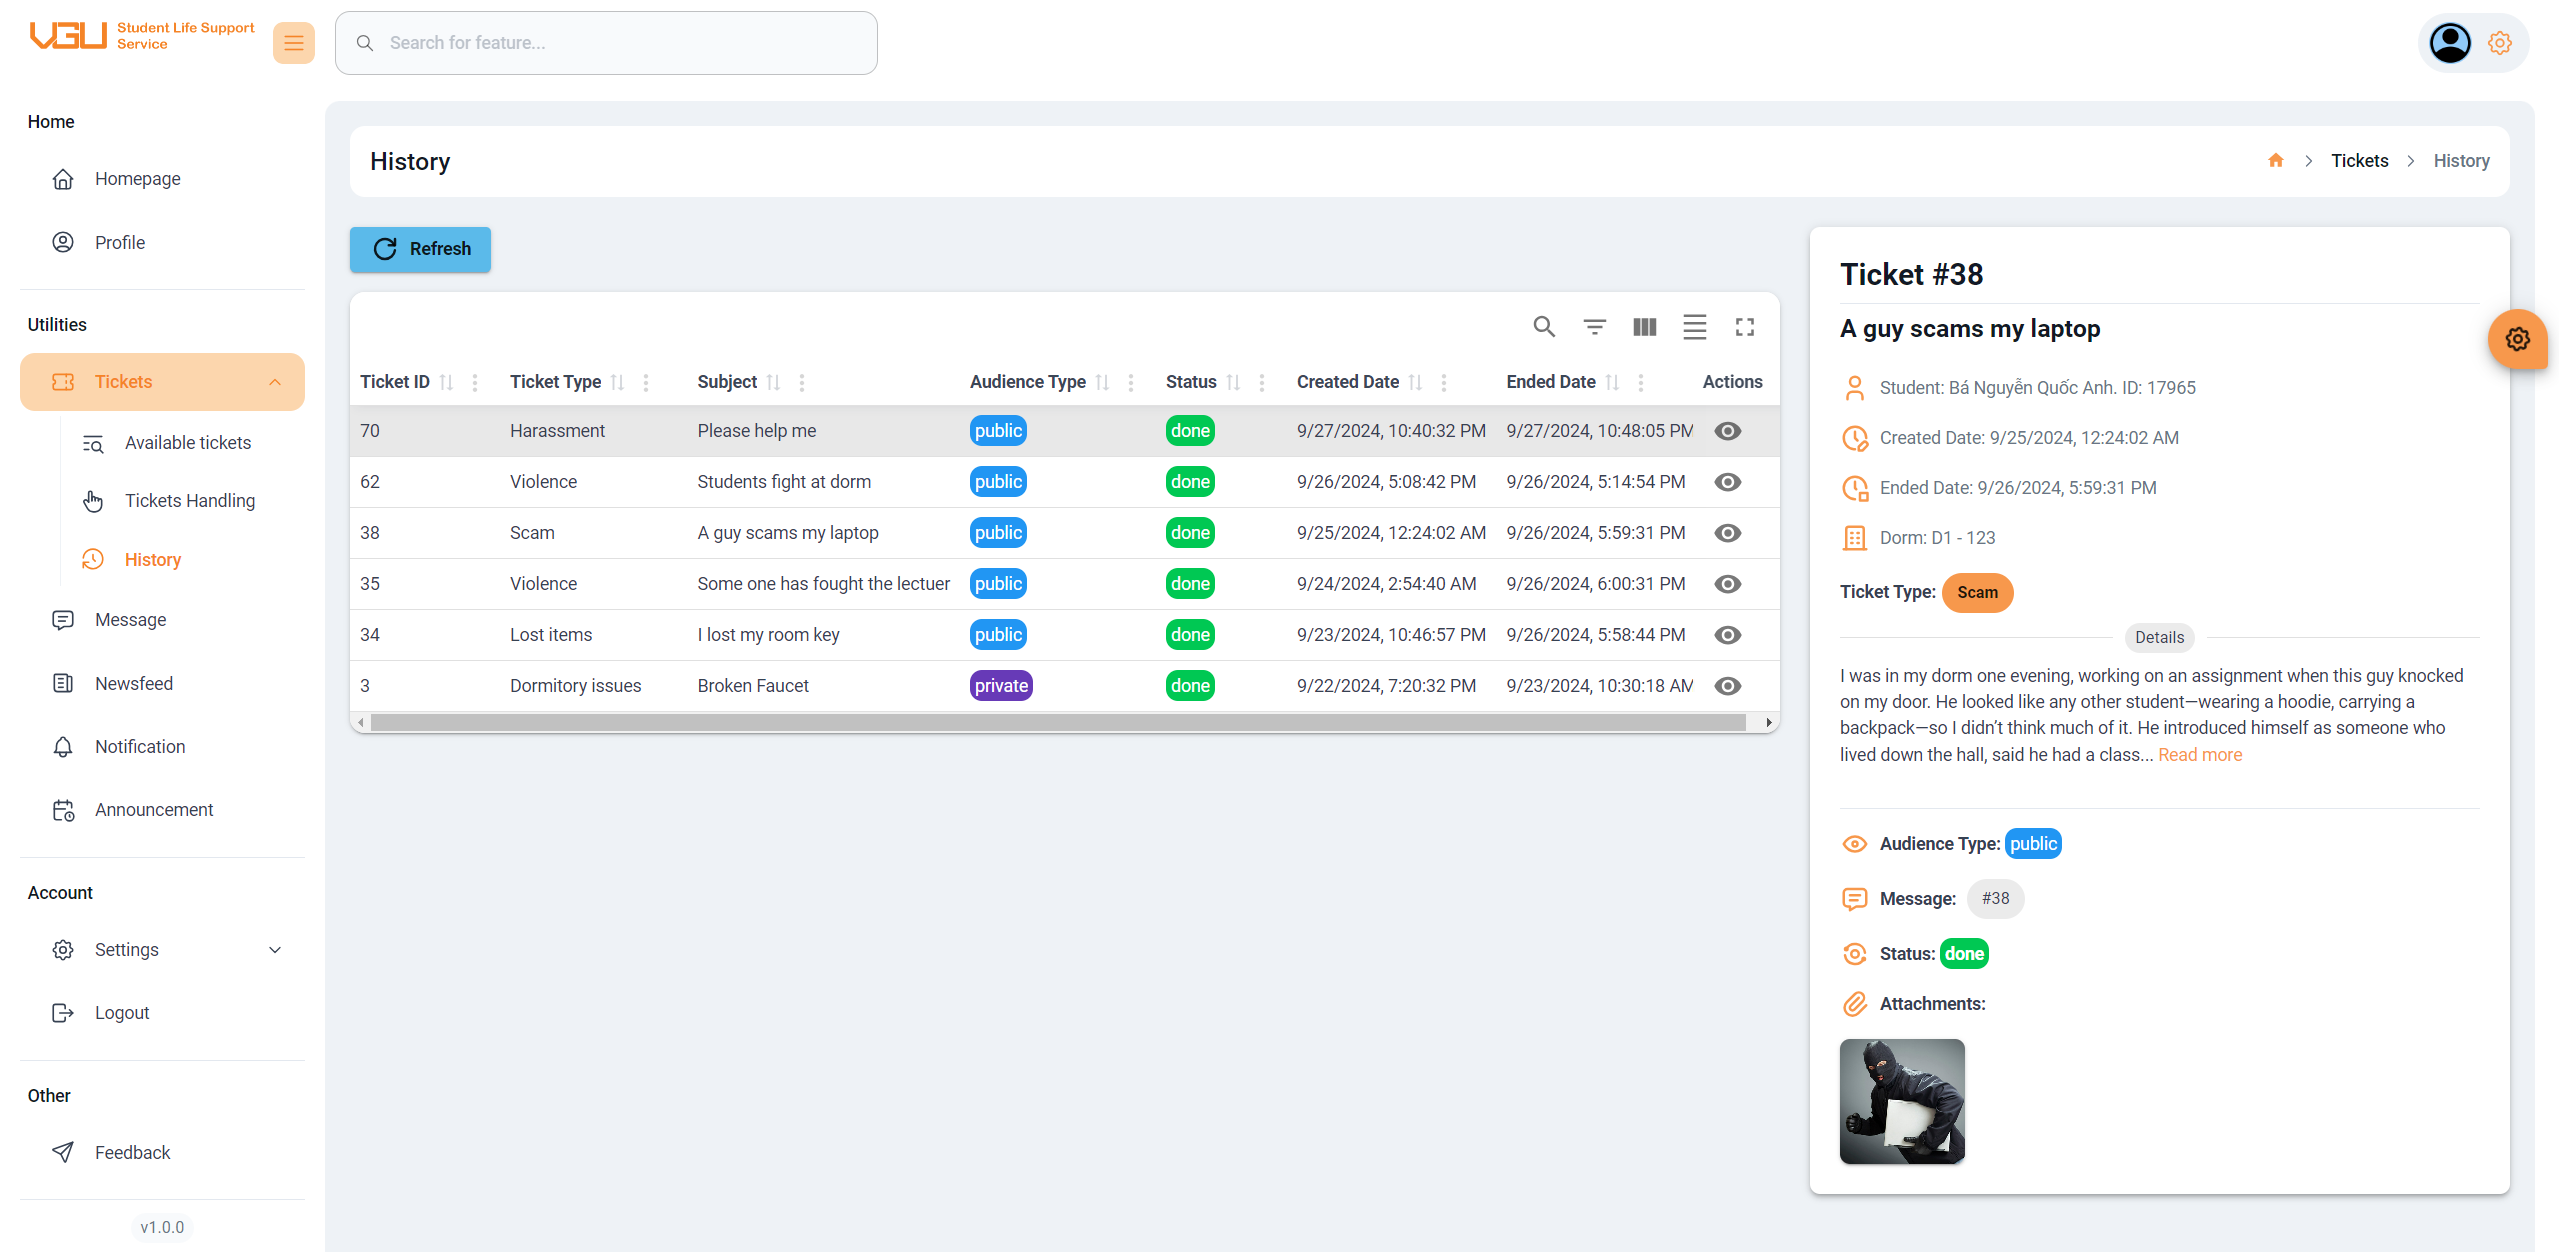
\includegraphics[width=1\linewidth]{graphics/gui/staff/ticket-history}
		\caption{Staff's Tickets History Page}
		\label{fig:gui-st-ticket-history}
	\end{figure}
	
	
	\subsubsection{Message}
	Staff members have the ability to communicate directly with students regarding specific tickets through the "Message" menu. This feature enables staff to send personalized messages to students associated with a particular ticket, facilitating clearer communication and providing necessary updates or clarifications. By selecting the relevant ticket, staff can compose messages that address the student's concerns, offer guidance, or request additional information if needed. This direct messaging capability not only enhances the support experience for students but also fosters a collaborative environment where staff can ensure that students are well-informed throughout the ticket resolution process. (Figure \ref{fig:gui-st-message})
	\begin{figure}[H]
		\centering
		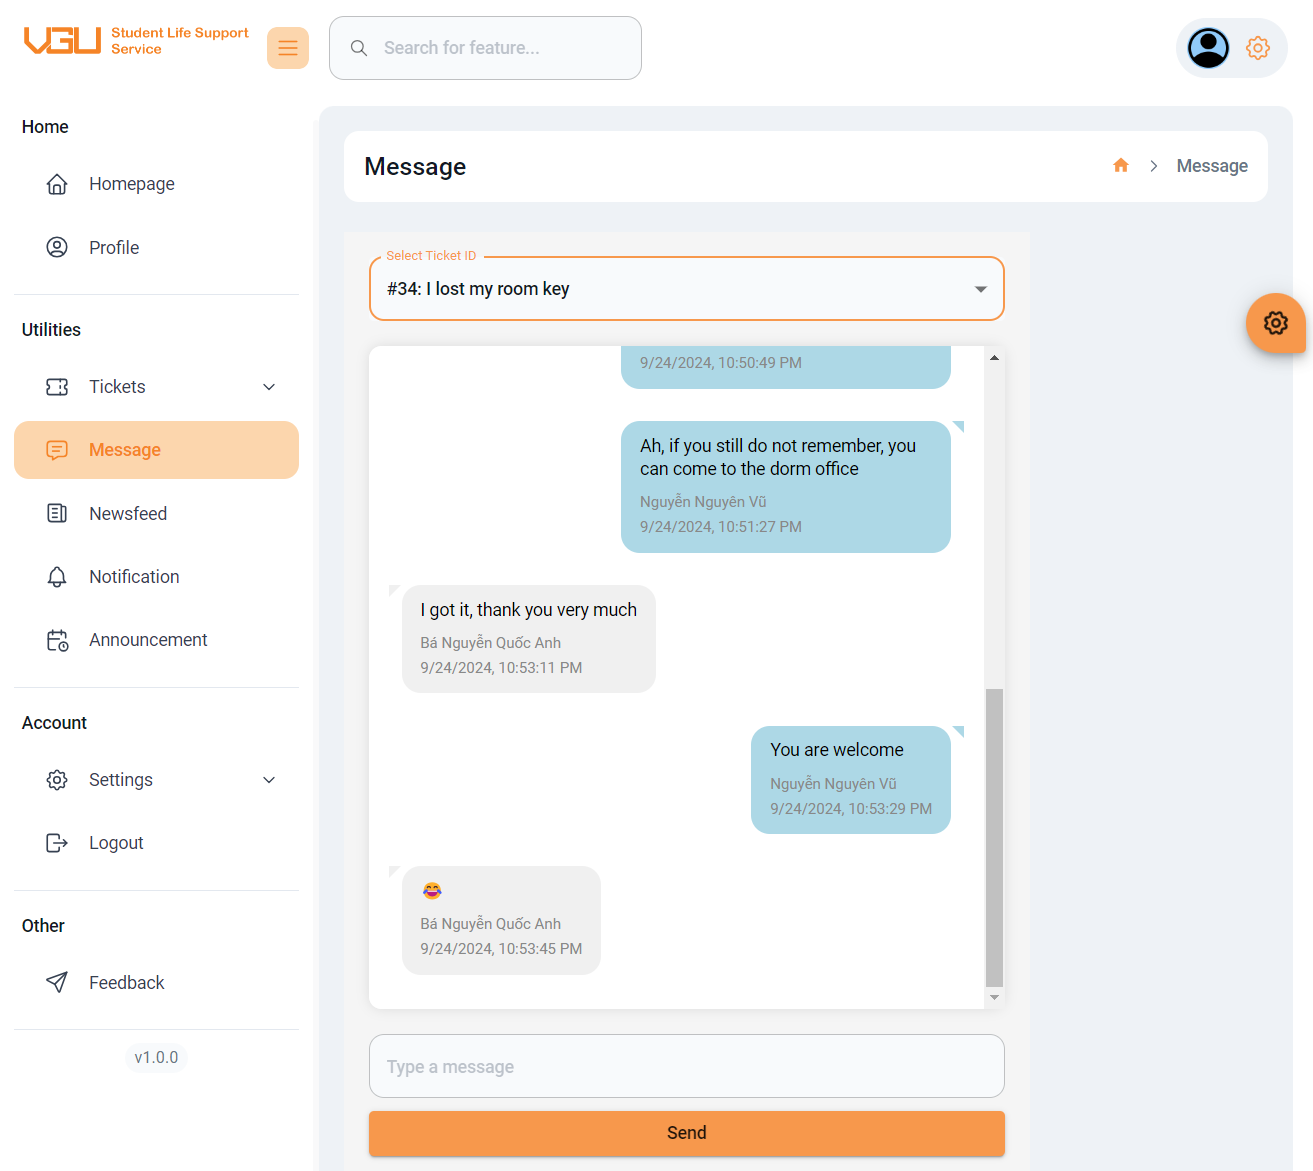
\includegraphics[width=1\linewidth]{graphics/gui/staff/message}
		\caption{Staff's Message Page}
		\label{fig:gui-st-message}
	\end{figure}
	
	\subsubsection{Notification}
	In addition to viewing existing notifications, staff members have the capability to create new notifications for various purposes. This functionality allows staff to disseminate important information, updates, or alerts to students and other relevant parties effectively. By utilizing the notification creation feature, staff can ensure that critical announcements reach their intended audience in a timely manner. Whether it's communicating changes in policies, upcoming events, or any other significant news, the ability to create notifications enhances the overall communication strategy within the system. 
%	\begin{figure}[H]
%		\centering
%		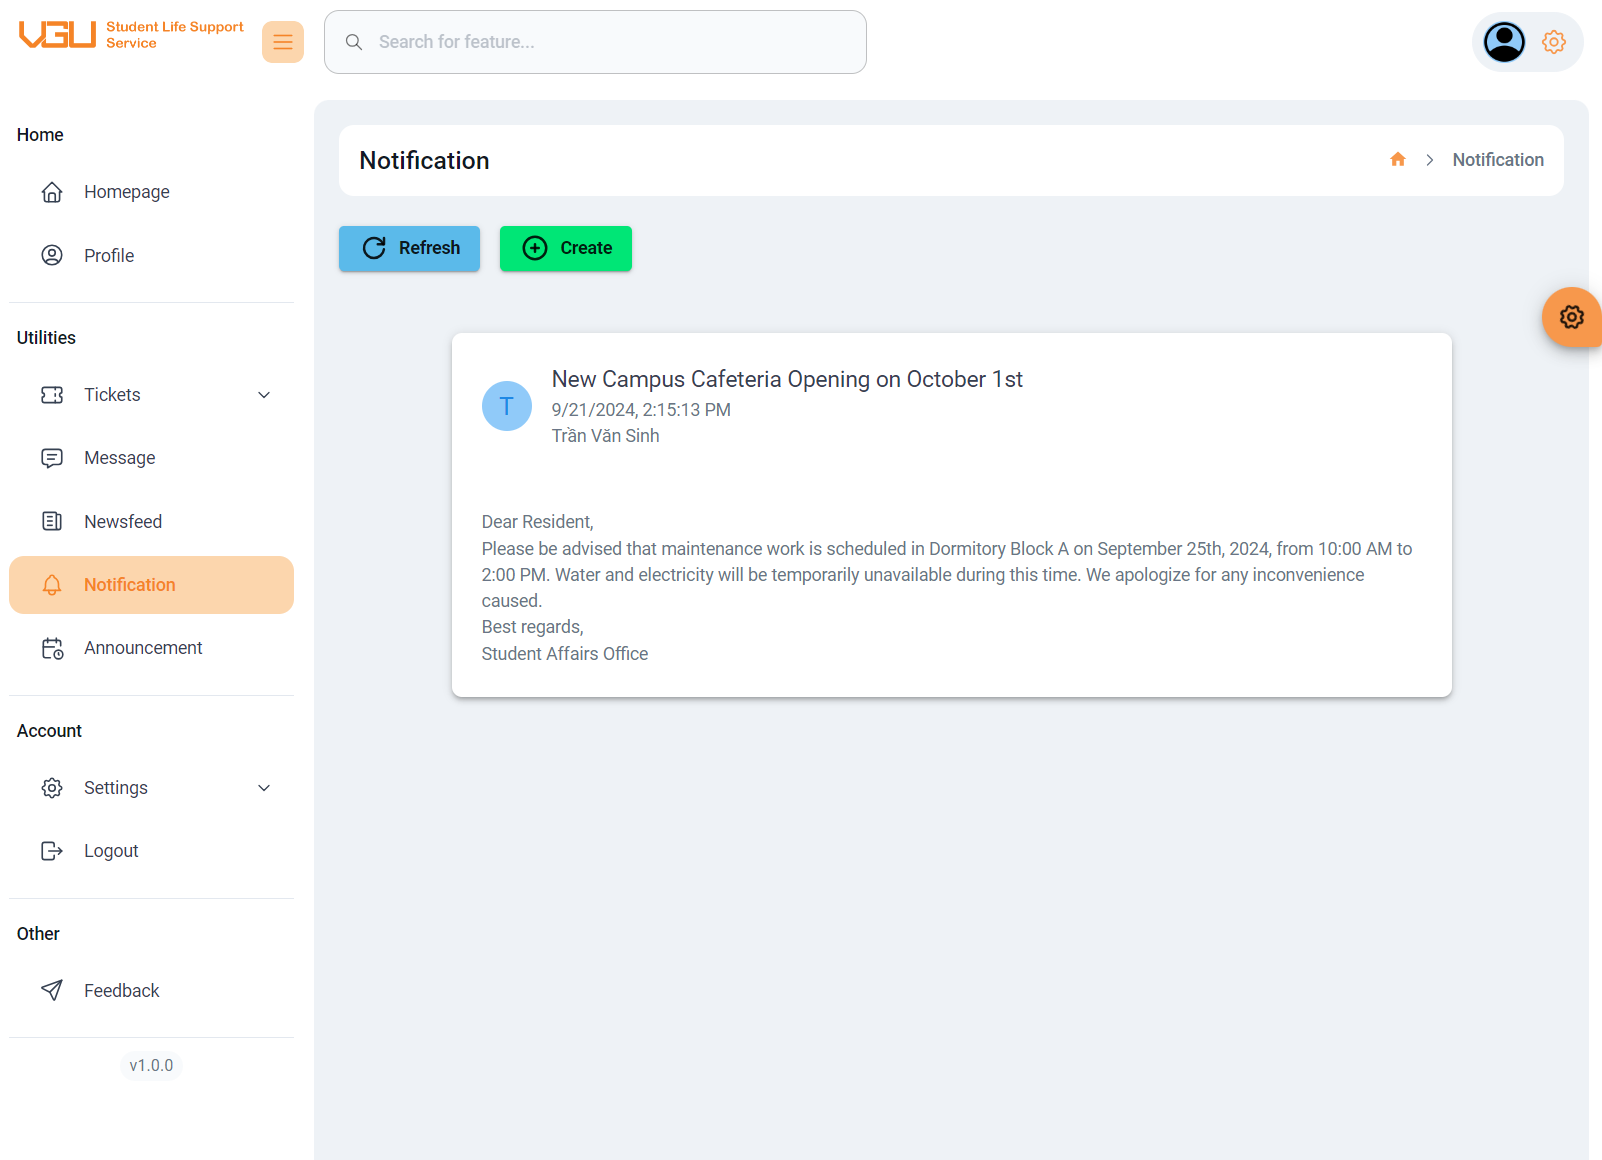
\includegraphics[width=1\linewidth]{graphics/gui/staff/notification}
%		\caption{Staff's Notification Page}
%		\label{fig:gui-st-notification}
%	\end{figure}
%	
	
	\begin{figure}[H]
		\centering
		\includegraphics[width=0.5\linewidth]{graphics/gui/staff/notìication-create}
		\caption{Create a Notification Modal}
		\label{fig:gui-st-notiication-create}
	\end{figure}
	
	\noindent Staff can tailor the content of the notification to suit specific needs, ensuring that the information is clear and relevant to the recipients. This proactive approach to communication helps maintain an informed community and encourages engagement among students and staff alike.
	

	
	
	\subsubsection{Announcement}
	
	In addition to being able to view existing announcements, staff members also have the option to create new announcements as needed. This feature empowers staff to communicate important updates, news, or information to students and other stakeholders effectively. By utilizing the announcement creation functionality, staff can share relevant details about events, policy changes, or any critical developments within the institution.
	\begin{figure}[H]
		\centering
		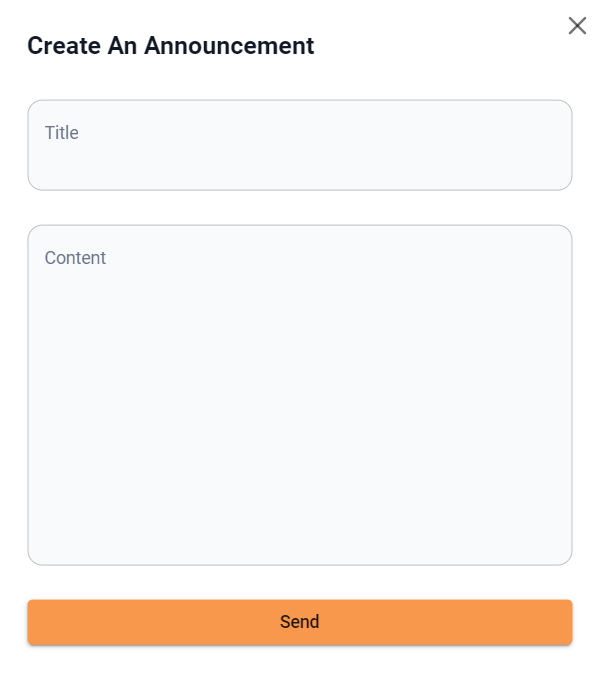
\includegraphics[width=0.5\linewidth]{graphics/gui/staff/announcement-create}
		\caption{Create an Announcement Modal}
		\label{fig:gui-st-announcement-create}
	\end{figure}
	
	\noindent The ability to craft announcements allows staff to ensure that their messages are clear, concise, and tailored to the audience they wish to reach. This not only fosters transparency within the organization but also keeps students informed and engaged with the latest happenings. Through the creation of announcements, staff can play a vital role in enhancing communication and ensuring that important information is readily accessible to all members of the community. Overall, this capability supports an open and informative environment, contributing to a more connected and responsive academic community.
	
	
\subsection{Admin's functions}
	\subsubsection{Tickets Management}
	Administrators possess the authority to oversee and manage all tickets within the Tickets Management section of the system. This functionality enables them to access a comprehensive list of all existing tickets, providing a clear overview of the current support requests submitted by users. \\ \\
	In addition to simply viewing these tickets, administrators have the capability to delete any tickets that have not received approval or are deemed invalid. This ensures that the ticketing system remains organized and efficient, as it helps to eliminate clutter caused by unnecessary or unapproved tickets. By actively managing the ticketing process, administrators can maintain the integrity of the system, ensuring that only legitimate and relevant tickets are processed. \\ \\ 
	This management feature not only enhances the overall user experience but also streamlines the workflow for support staff, allowing them to focus on valid tickets that require attention. Ultimately, this proactive approach to ticket management fosters a more efficient and effective support environment, benefiting both administrators and users alike.
	\begin{figure}[H]
		\centering
		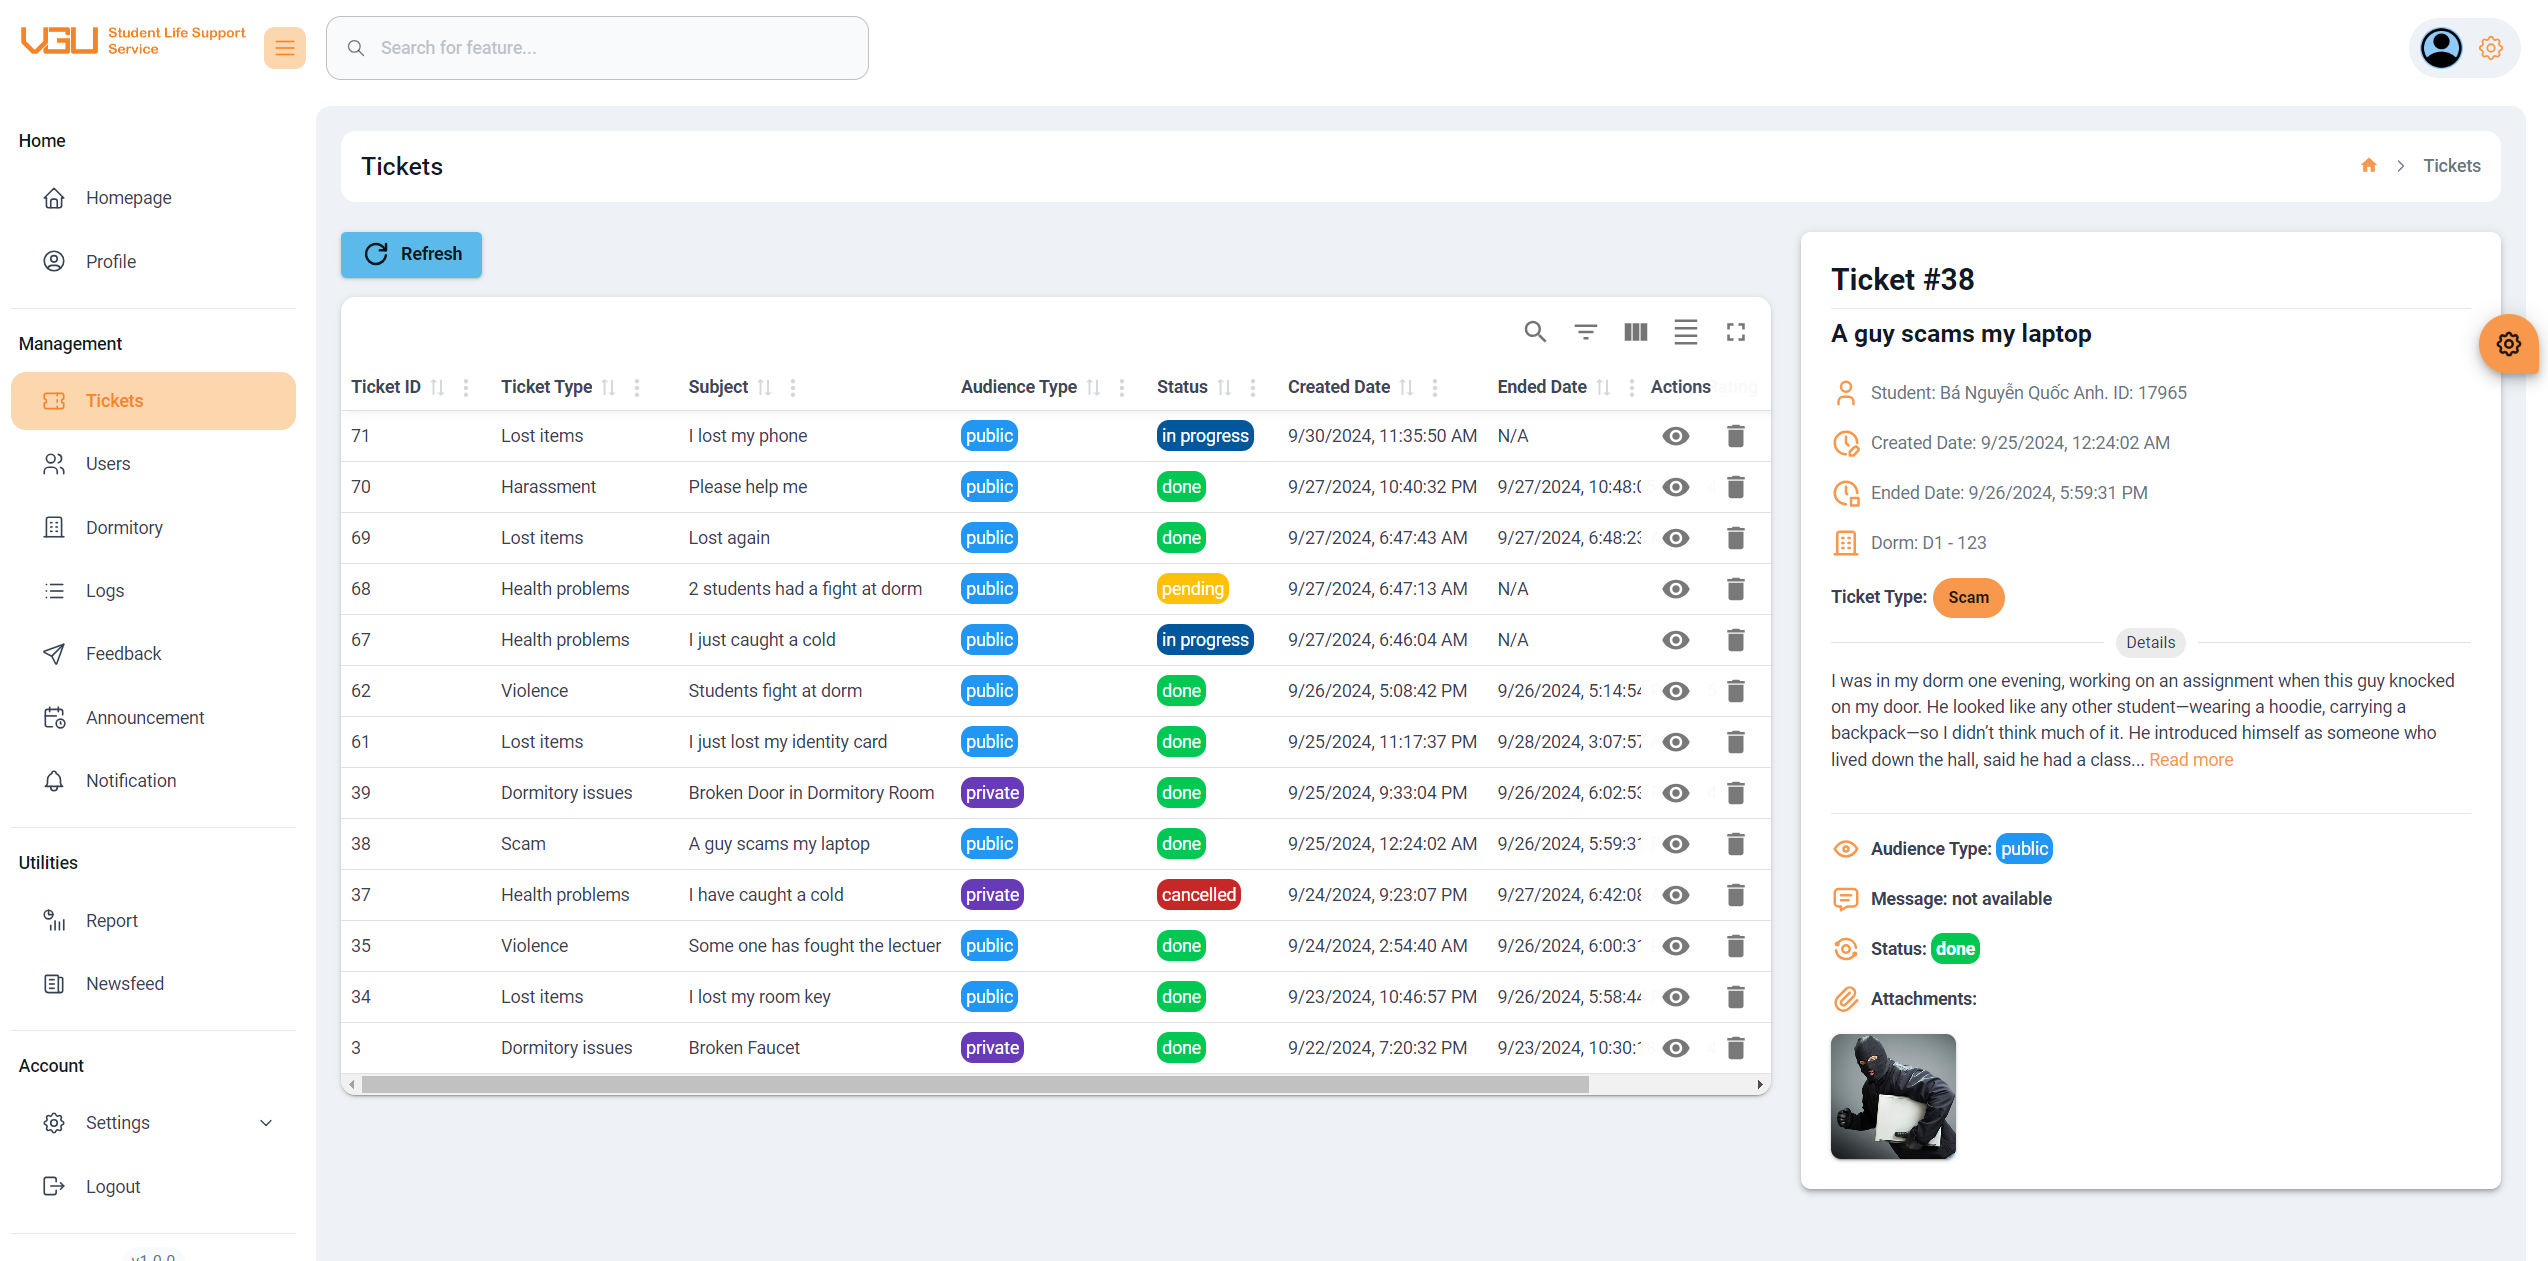
\includegraphics[width=1\linewidth]{graphics/gui/admin/ticket-mng}
		\caption{Admin's Ticket Management Page}
		\label{fig:gui-ad-ticket-mng}
	\end{figure}
	
	
	\subsubsection{Users Management}
	Administrators have comprehensive access to the user management functionalities within the system. They are able to view all registered users, which allows them to monitor user activity and maintain an overview of the community within the platform. This capability ensures that administrators can identify any potential issues or areas that require attention among the user base. \\ \\ 
	In addition to merely viewing users, administrators also have the authority to create new user accounts as needed. This feature is particularly useful for onboarding new members, whether they are students, staff, or other stakeholders who require access to the system. Furthermore, administrators can edit the information of existing users, including updating personal details and modifying user roles as necessary. This flexibility is crucial for adapting to changes in user responsibilities or correcting any inaccuracies in user profiles. \\ \\
	Moreover, administrators possess the ability to delete user accounts if required, particularly in cases where users are no longer active or if there are concerns regarding compliance with system policies. This feature aids in maintaining the security and integrity of the system by ensuring that only authorized users have access.
	
	\begin{figure}[H]
		\centering
		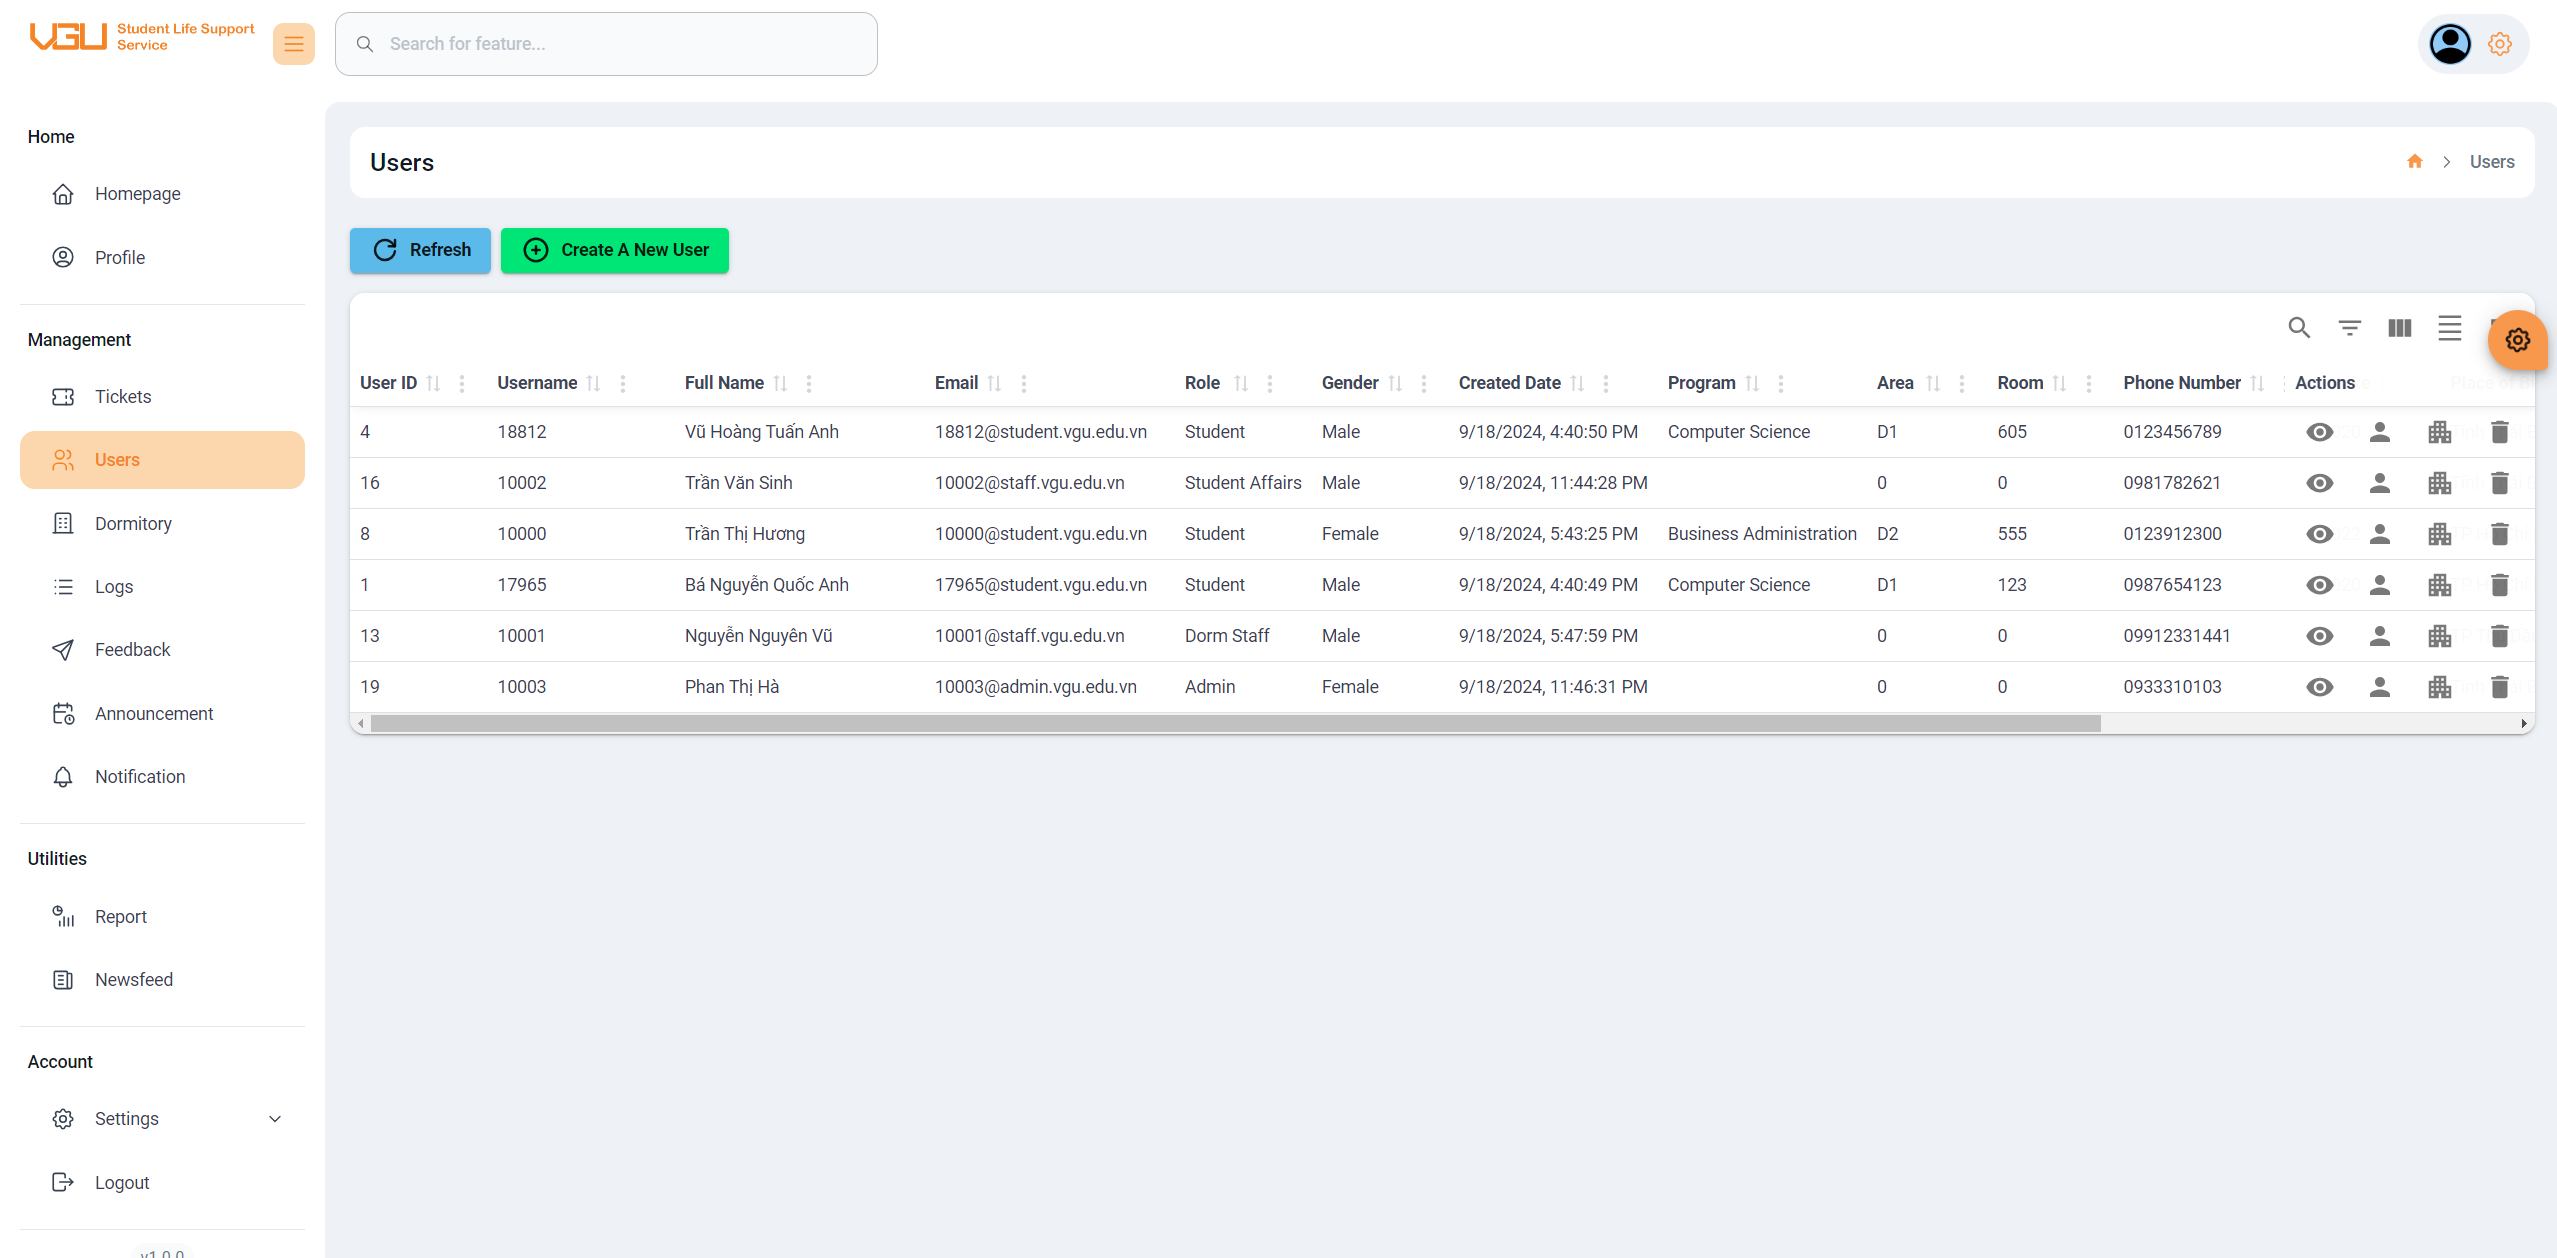
\includegraphics[width=1\linewidth]{graphics/gui/admin/user-mng}
		\caption{Admin's User Management Page}
		\label{fig:gui-ad-user-mng}
	\end{figure}
	
	\subsubsection{Dormitory Management}
	Administrators have the ability to access and manage all dormitory information within the system, including viewing details such as occupancy rates and amenities. They can create new dorm entries when new facilities are established and delete outdated or erroneous entries to maintain data accuracy. This functionality ensures that the dormitory offerings are accurately represented and helps administrators efficiently oversee housing resources for users.
	\begin{figure}[H]
		\centering
		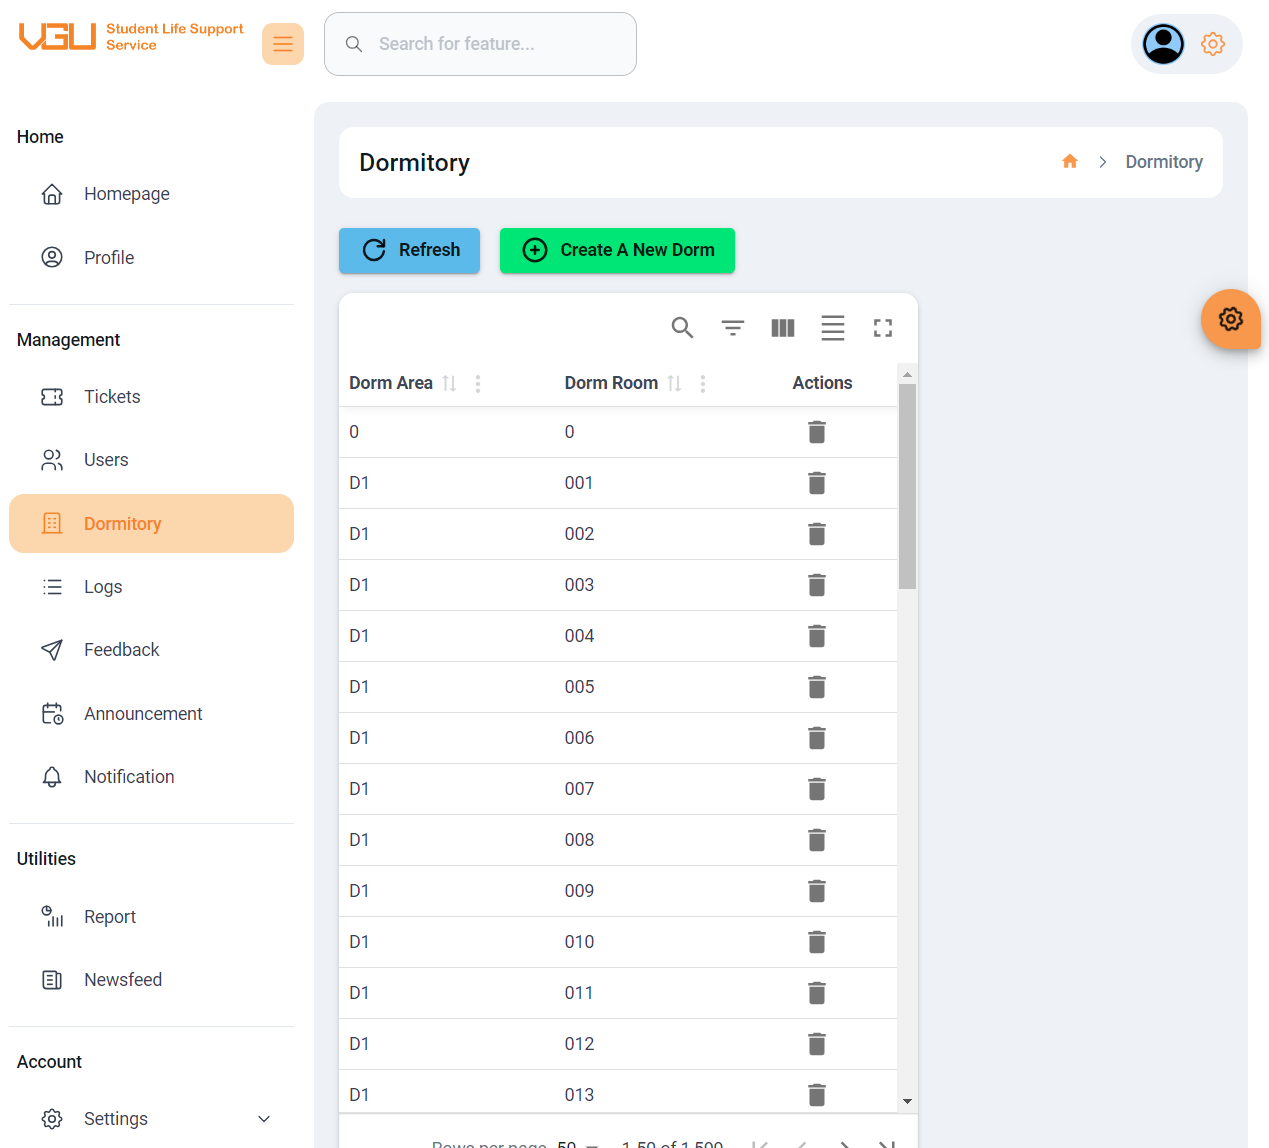
\includegraphics[width=0.9\linewidth]{graphics/gui/admin/dorm-mng}
		\caption{Admin's Dormitory Management Page}
		\label{fig:gui-ad-dorm-mng}
	\end{figure}
	
	
	\subsubsection{Logs Management}
	Administrators have the capability to access the complete system logs, which provide a detailed record of all activities and events occurring within the system. They can selectively delete individual logs if they find them unnecessary or opt to clear all logs at once to maintain a cleaner database. Additionally, administrators can export these logs in various formats, including CSV, PDF, or Excel, enabling easier analysis and reporting. This functionality ensures that administrators can efficiently manage log data while also retaining the flexibility to utilize the information in formats that best suit their needs.
	\begin{figure}[H]
		\centering
		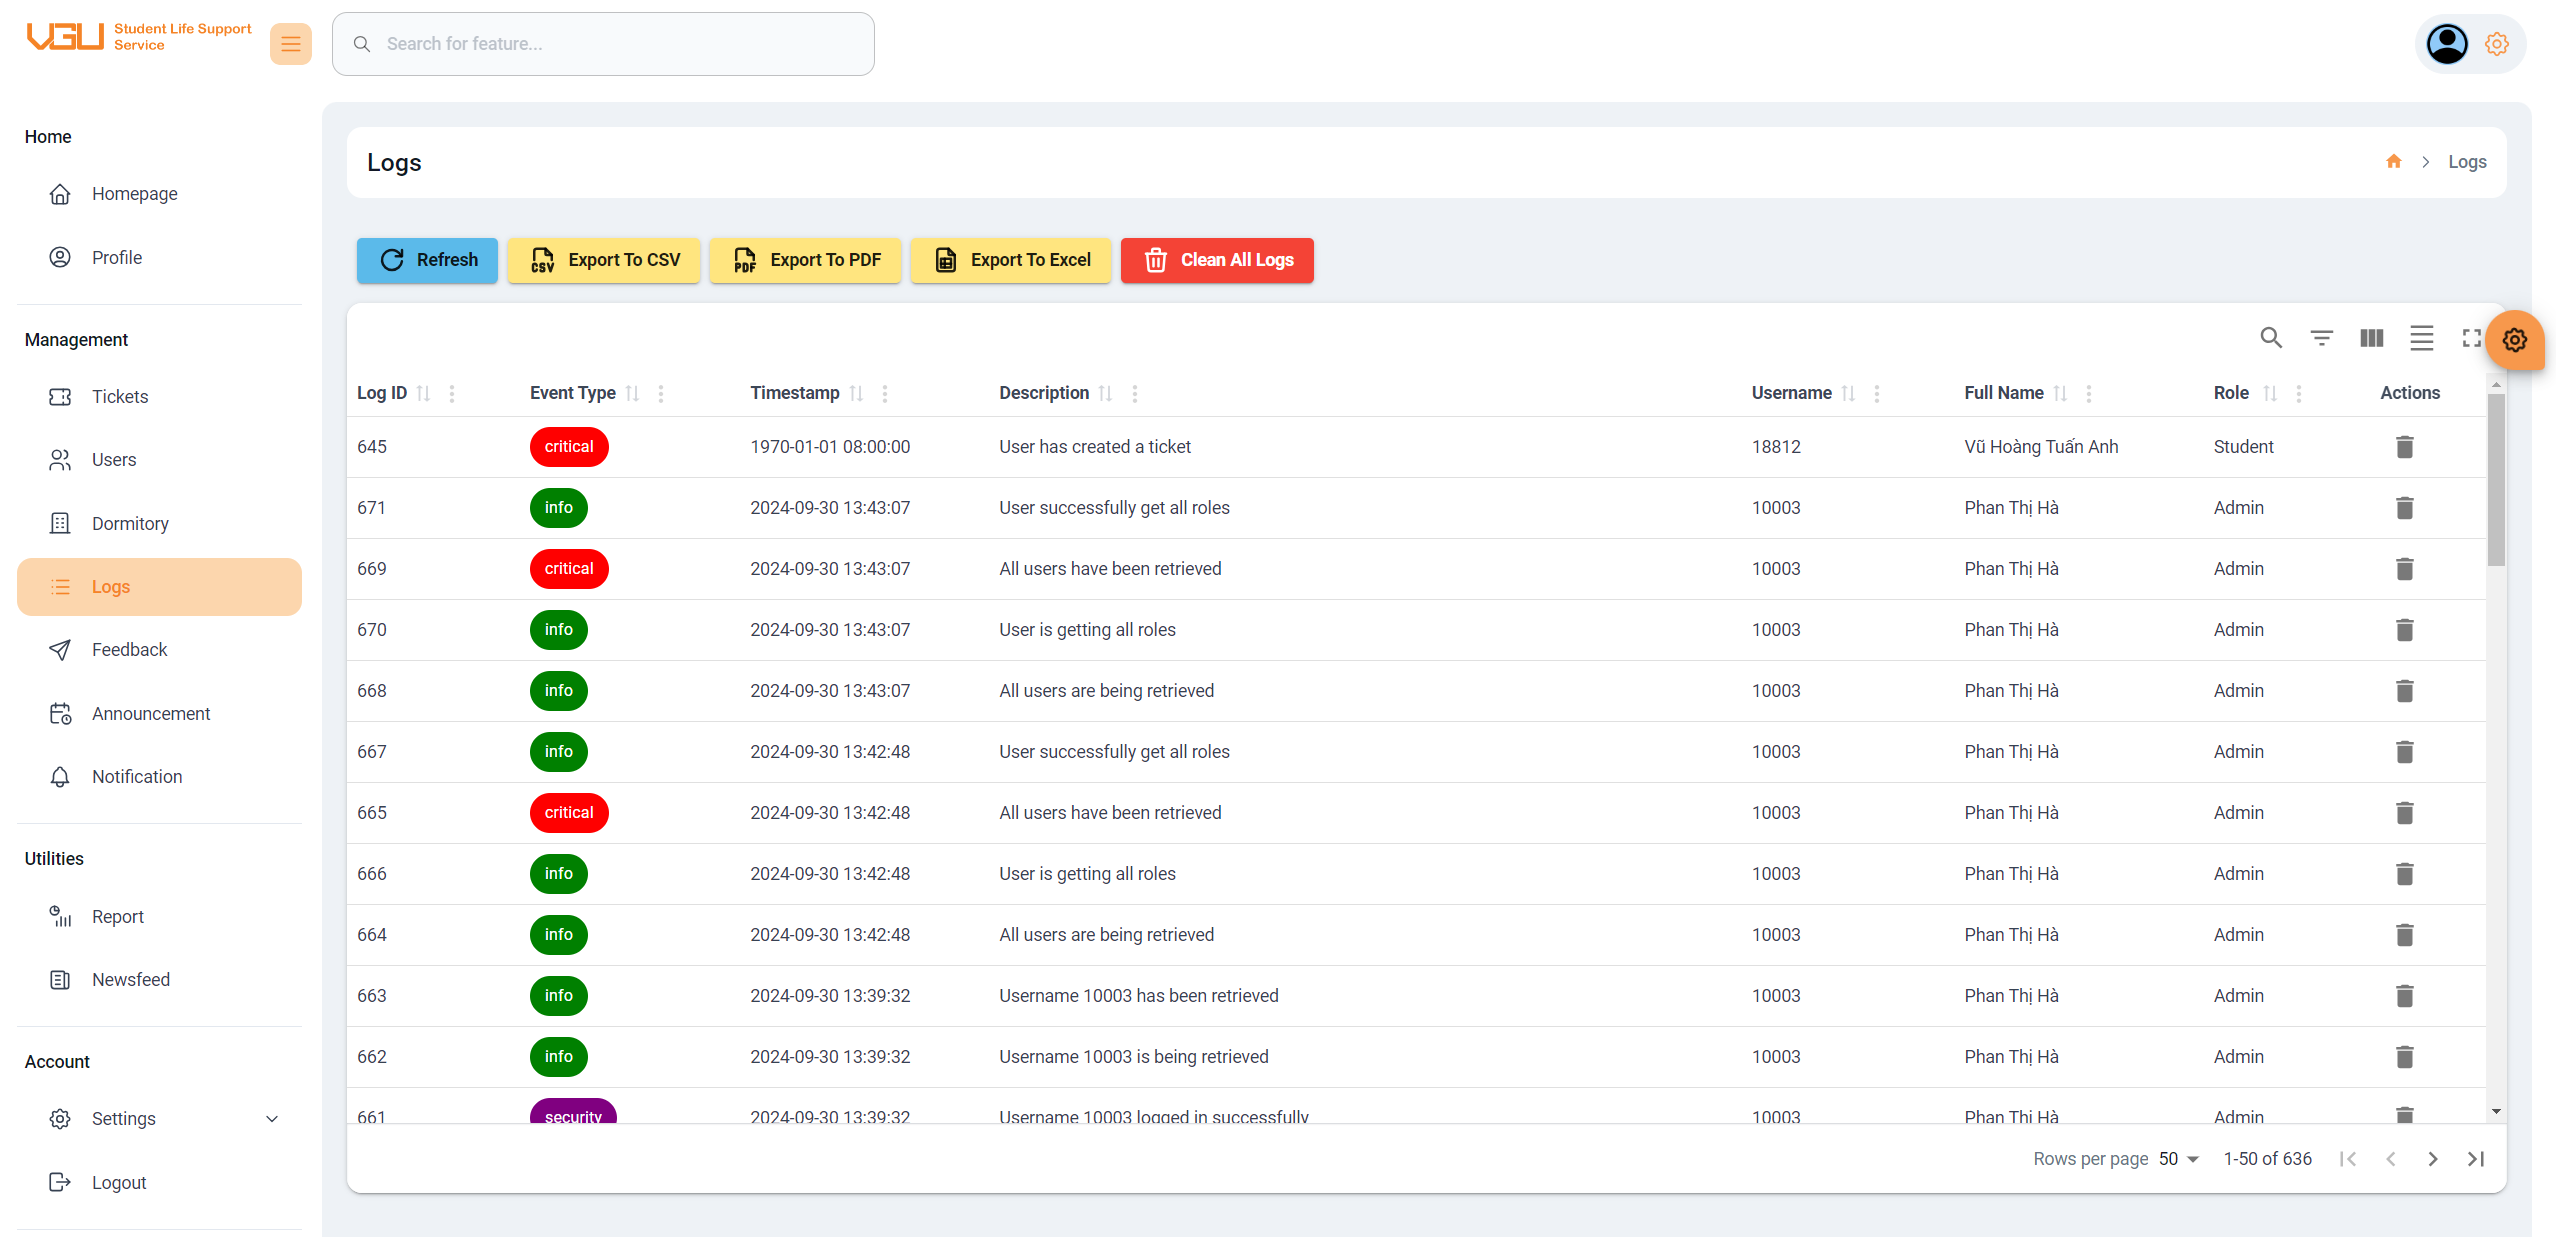
\includegraphics[width=1\linewidth]{graphics/gui/admin/logs-mng}
		\caption{Admin's Logs Management Page}
		\label{fig:gui-ad-logs-mng}
	\end{figure}
	
	
	\subsubsection{Feedback Management}
	Administrators have the ability to oversee and manage all feedback submitted by both students and staff members within the system. This includes viewing detailed comments, suggestions, and evaluations provided by users, as well as the corresponding feedback scores. By analyzing this information, administrators can gain valuable insights into the experiences and perspectives of users, helping them identify areas for improvement and enhance the overall functionality and user satisfaction of the system. This comprehensive management of feedback ensures that administrators remain informed about the sentiments and concerns of the user community.
	\begin{figure}[H]
		\centering
		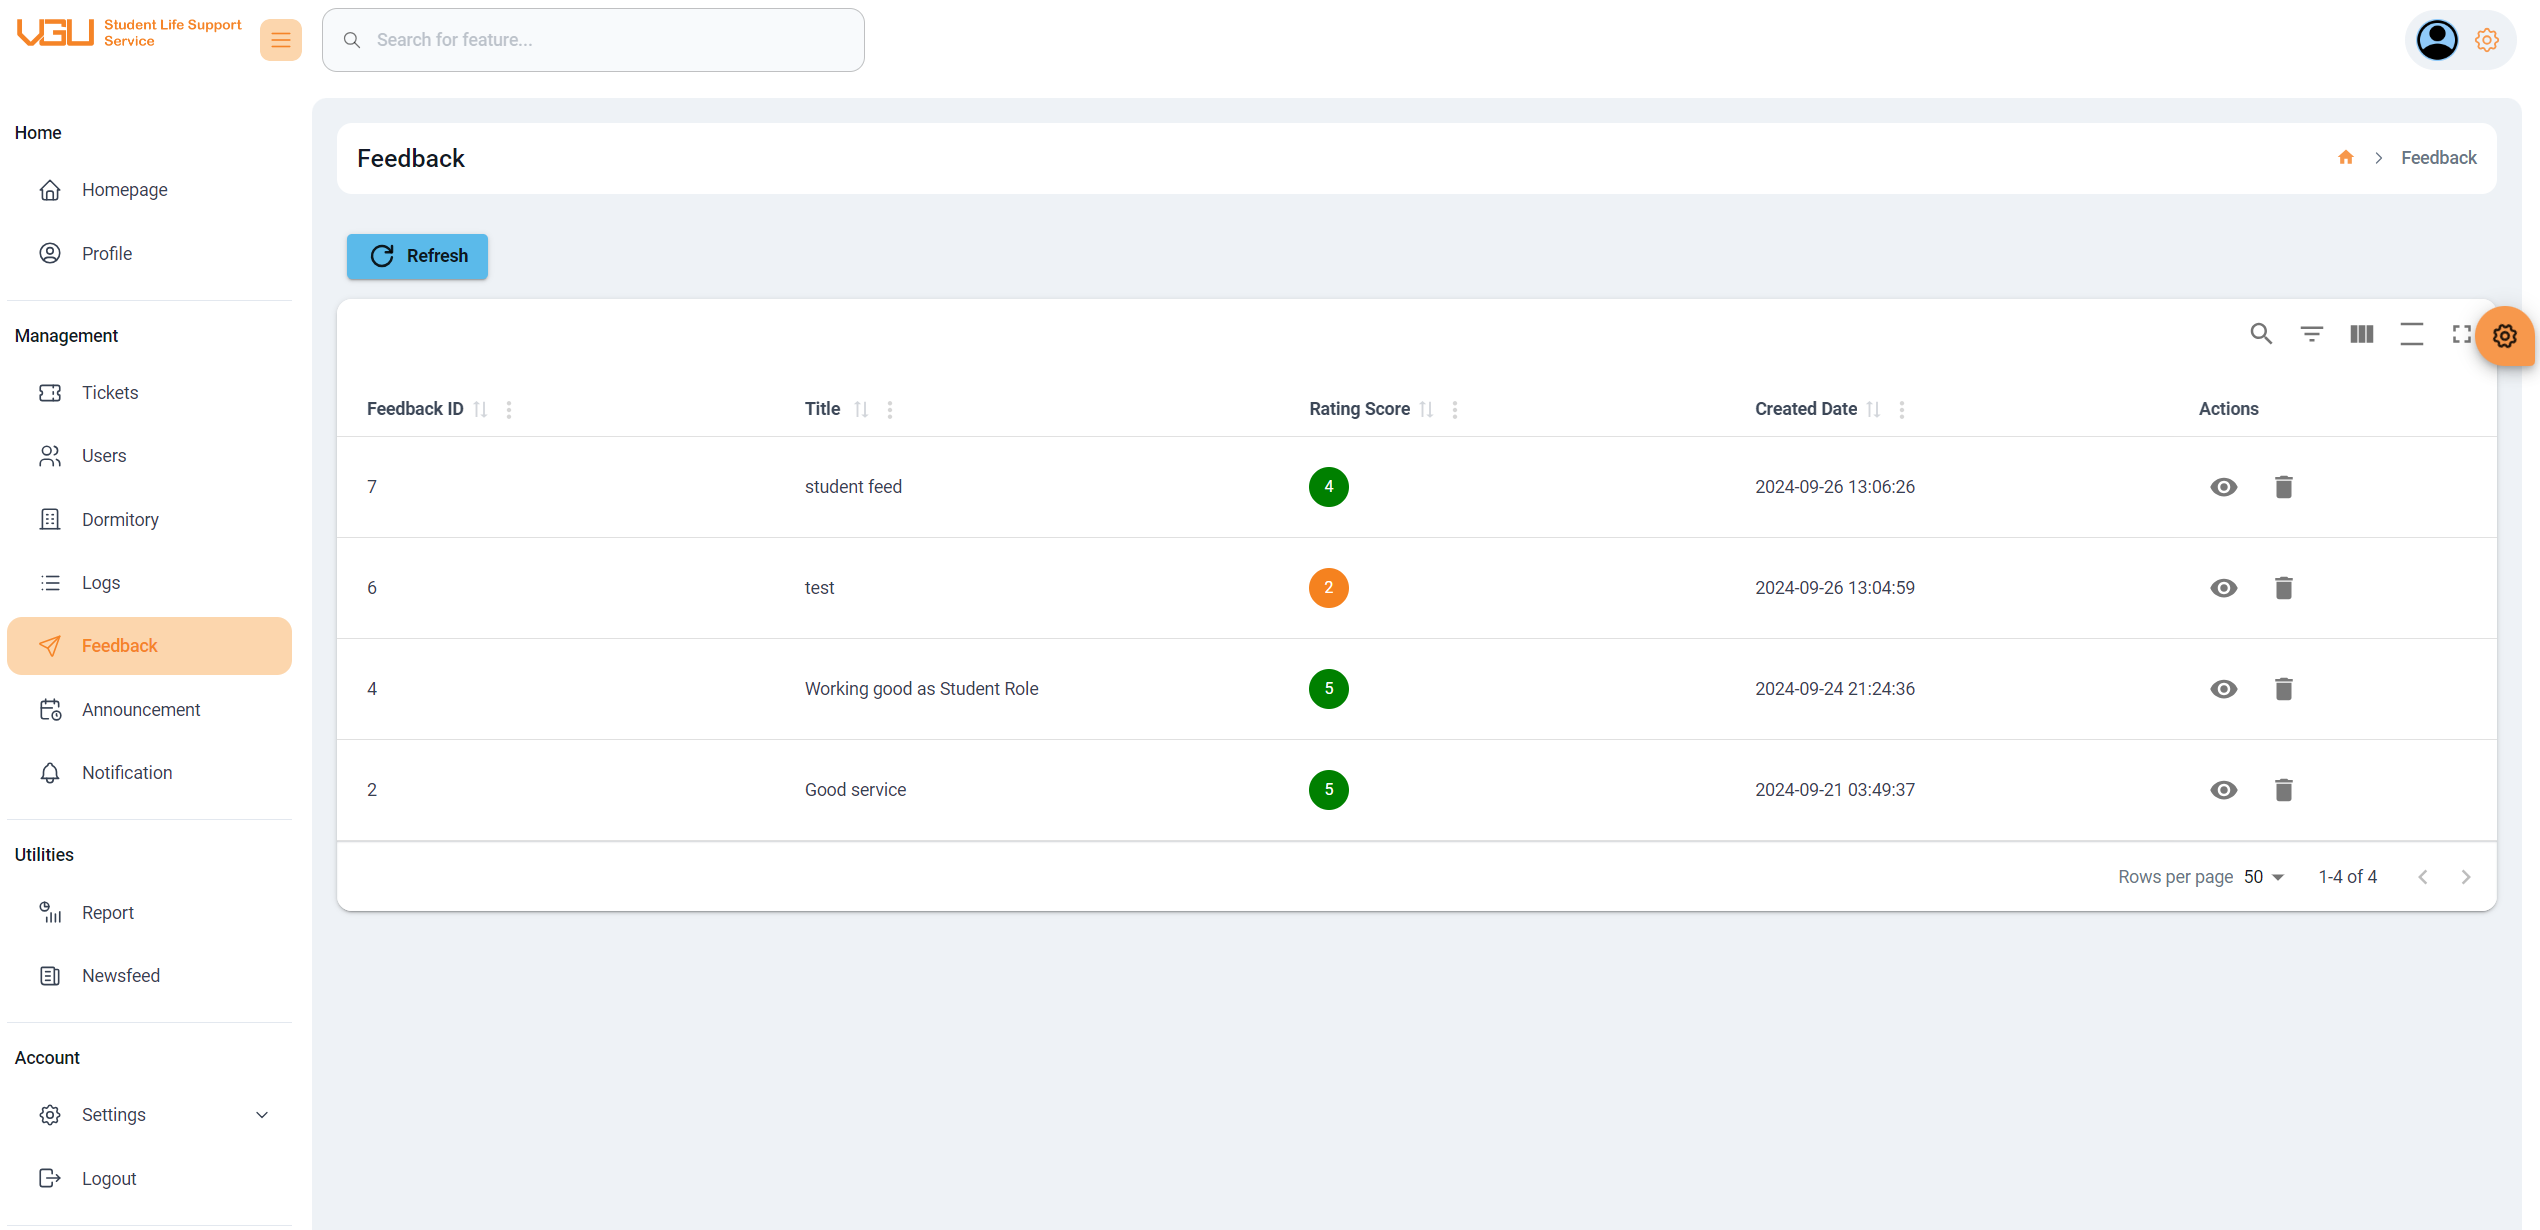
\includegraphics[width=1\linewidth]{graphics/gui/admin/feedback-mng}
		\caption{Admin's Feedback Management Page}
		\label{fig:feedback-mng}
	\end{figure}
	
	
	\subsubsection{Report}
	\begin{figure}[H]
		\centering
		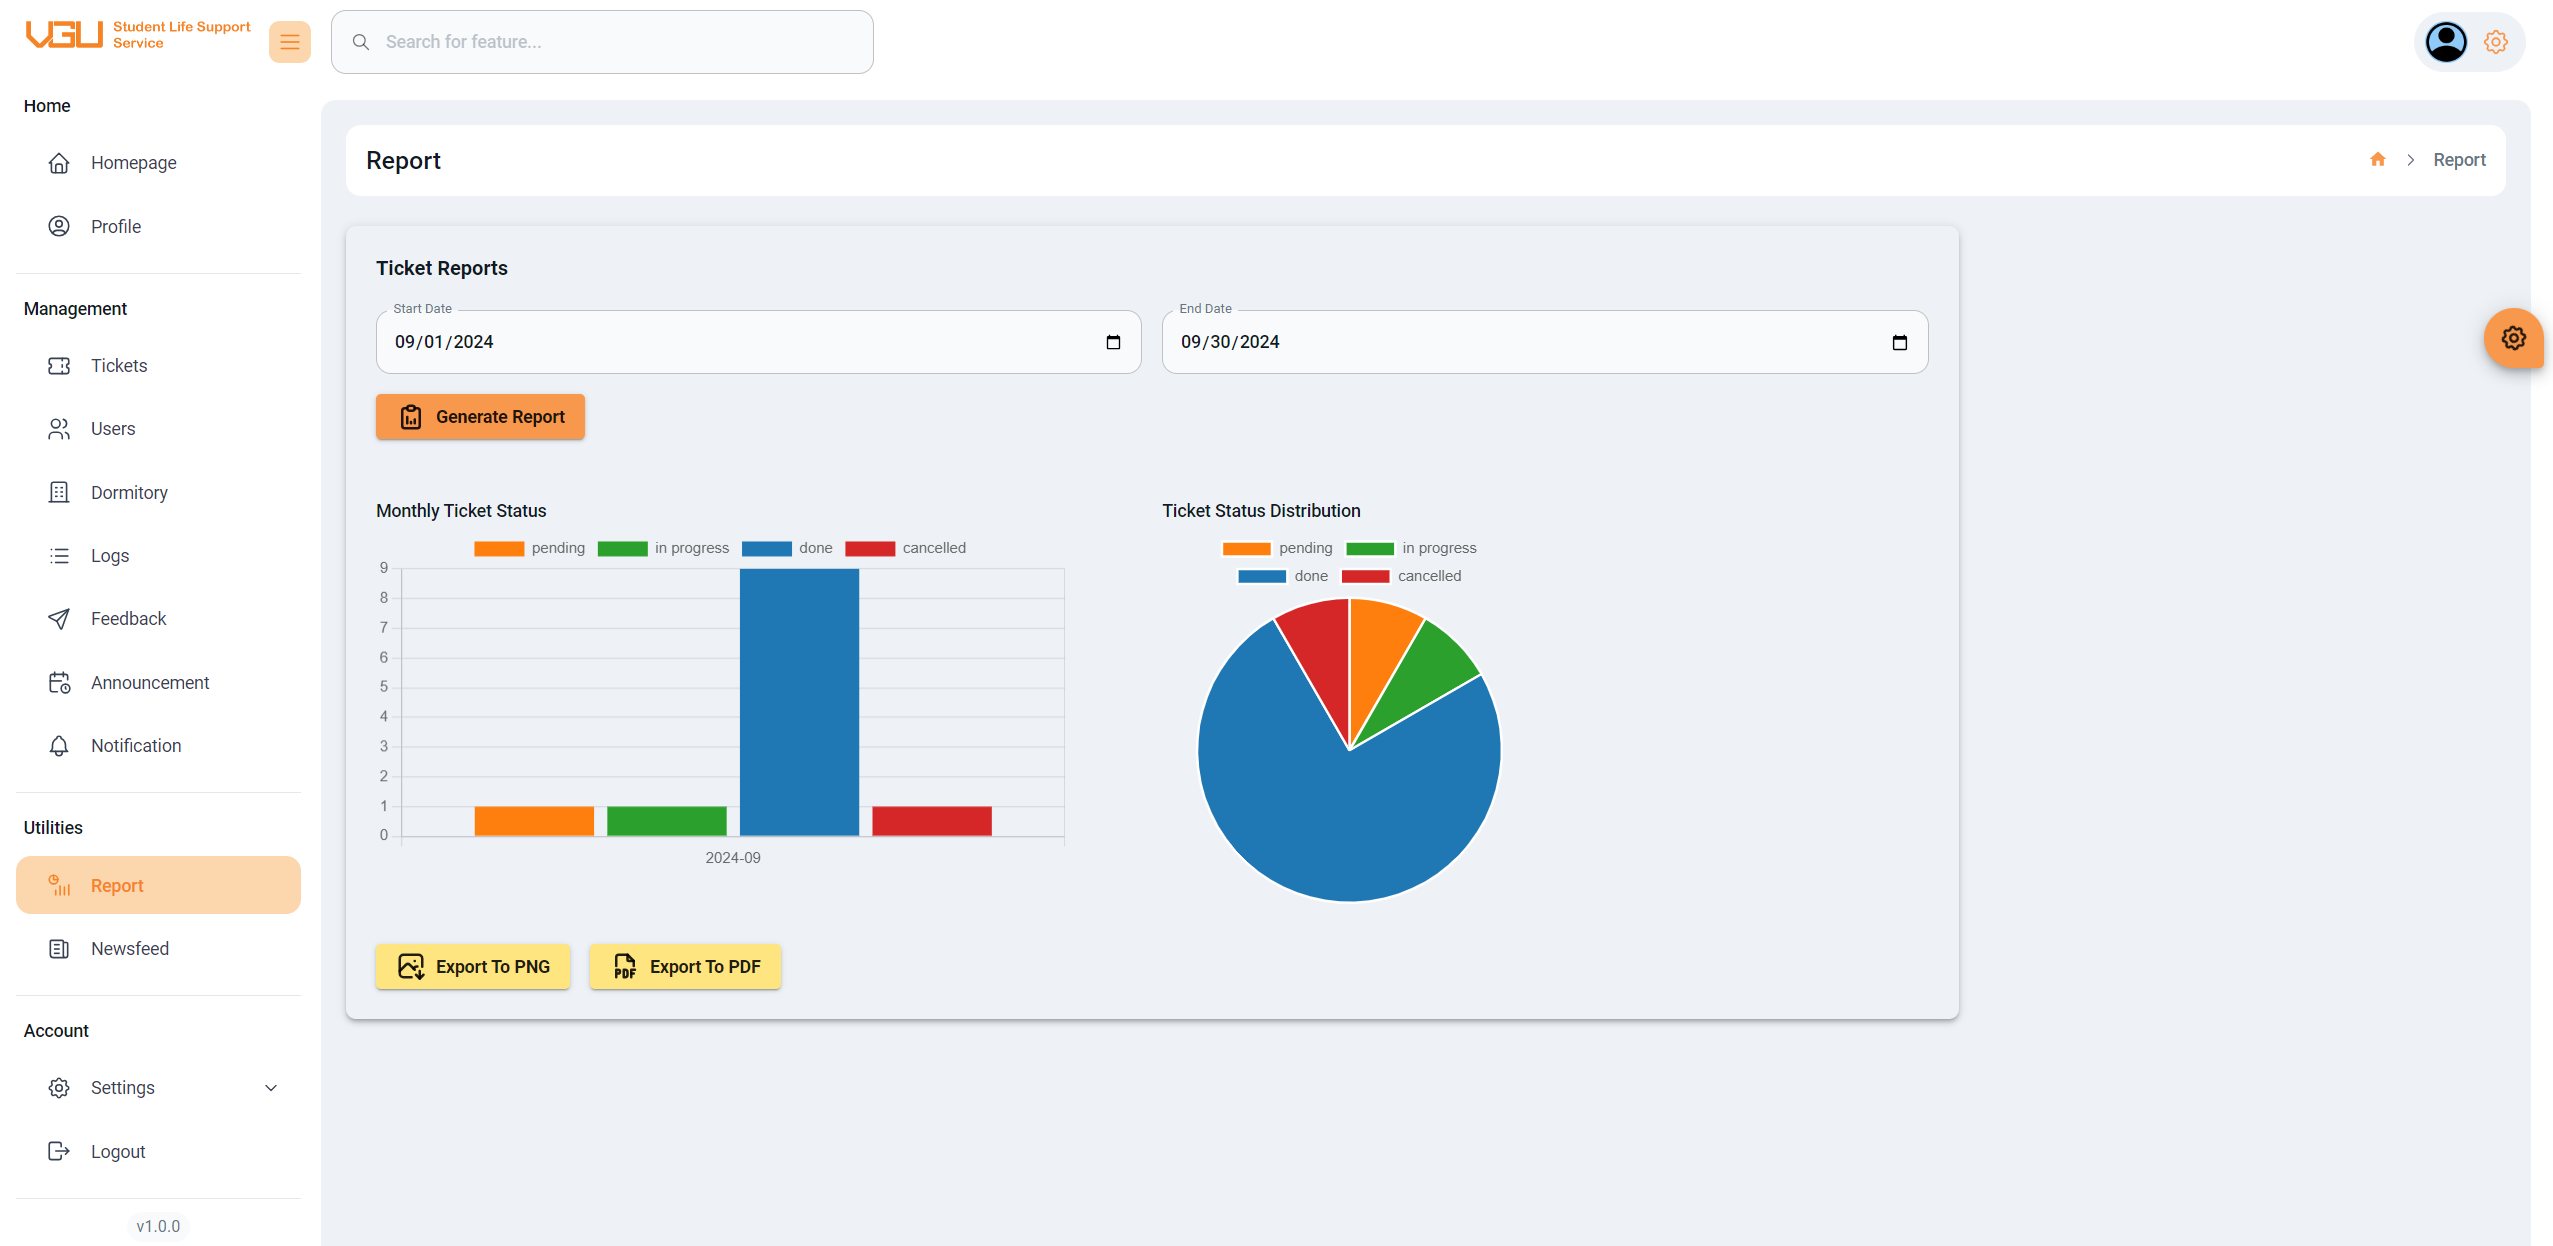
\includegraphics[width=1\linewidth]{graphics/gui/admin/report-util}
		\caption{Admin's Report Page}
		\label{fig:report-util}
	\end{figure}
	
	Administrators have the capability to generate detailed ticket reports for a specified time period, allowing them to analyze ticket activity and performance metrics during that interval. Once the report is created, administrators can easily export it in various formats, such as PNG or PDF. This functionality not only facilitates efficient record-keeping but also enables administrators to share insights and data with stakeholders, ensuring that they are well-informed about ticket trends, resolutions, and user interactions within the system. By having access to these reports, administrators can make data-driven decisions to improve service delivery and address any issues effectively.
	
	
	
	
	
	
	
	
	
	
	

	
	
	
	
	
	
	
	
	
	



